% ******************************* PhD Thesis Template **************************
% Please have a look at the README.md file for info on how to use the template

\documentclass[a4paper,12pt,times,numbered,print,index]{PhDThesisPSnPDF}

% ******************************************************************************
% ******************************* Class Options ********************************
% *********************** See README for more details **************************
% ******************************************************************************

% `a4paper'(The University of Cambridge PhD thesis guidelines recommends a page
% size a4 - default option) or `a5paper': A5 Paper size is also allowed as per
% the Cambridge University Engineering Department guidelines for PhD thesis
%
% `11pt' or `12pt'(default): Font Size 10pt is NOT recommended by the University
% guidelines
%
% `oneside' or `twoside'(default): Printing double side (twoside) or single
% side.
%
% `print': Use `print' for print version with appropriate margins and page
% layout. Leaving the options field blank will activate Online version.
%
% `index': For index at the end of the thesis
%
% `draftclassic': For draft mode without loading any images (same as draft in book)
%
% `draft': Special draft mode with line numbers, images, and water mark with
% timestamp and custom text. Position of the text can also be modified.
%
% `abstract': To generate only the title page and abstract page with
% dissertation title and name, to submit to the Student Registry
%
% `chapter`: This option enables only the specified chapter and its references
%  Useful for review and corrections.
%
% ************************* Custom Page Margins ********************************
%
% `custommargin`: Use `custommargin' in options to activate custom page margins,
% which can be defined in the preamble.tex. Custom margin will override
% print/online margin setup.
%
% *********************** Choosing the Fonts in Class Options ******************
%
% `times' : Times font with math support. (The Cambridge University guidelines
% recommend using times)
%
% `fourier': Utopia Font with Fourier Math font (Font has to be installed)
%            It's a free font.
%
% `customfont': Use `customfont' option in the document class and load the
% package in the preamble.tex
%
% default or leave empty: `Latin Modern' font will be loaded.
%
% ********************** Choosing the Bibliography style ***********************
%
% `authoryear': For author-year citation eg., Krishna (2013)
%
% `numbered': (Default Option) For numbered and sorted citation e.g., [1,5,2]
%
% `custombib': Define your own bibliography style in the `preamble.tex' file.
%              `\RequirePackage[square, sort, numbers, authoryear]{natbib}'.
%              This can be also used to load biblatex instead of natbib
%              (See Preamble)
%
% **************************** Choosing the Page Style *************************
%
% `default (leave empty)': For Page Numbers in Header (Left Even, Right Odd) and
% Chapter Name in Header (Right Even) and Section Name (Left Odd). Blank Footer.
%
% `PageStyleI': Chapter Name next & Page Number on Even Side (Left Even).
% Section Name & Page Number in Header on Odd Side (Right Odd). Footer is empty.
%
% `PageStyleII': Chapter Name on Even Side (Left Even) in Header. Section Number
% and Section Name in Header on Odd Side (Right Odd). Page numbering in footer

% Uncomment to change page style
%\pagestyle{PageStyleII}

% ********************************** Preamble **********************************
% Preamble: Contains packages and user-defined commands and settings
% ******************************************************************************
% ****************************** Custom Margin *********************************

% Add `custommargin' in the document class options to use this section
% Set {innerside margin / outerside margin / topmargin / bottom margin}  and
% other page dimensions
\ifsetCustomMargin
  \RequirePackage[left=37mm,right=30mm,top=35mm,bottom=30mm]{geometry}
  \setFancyHdr % To apply fancy header after geometry package is loaded
\fi

% Add spaces between paragraphs
%\setlength{\parskip}{0.5em}
\usepackage[skip=10pt plus1pt, indent=0pt]{parskip}
% Ragged bottom avoids extra whitespaces between paragraphs
\raggedbottom
% To remove the excess top spacing for enumeration, list and description
%\usepackage{enumitem}
%\setlist[enumerate,itemize,description]{topsep=0em}

% *****************************************************************************
% ******************* Fonts (like different typewriter fonts etc.)*************

% Add `customfont' in the document class option to use this section

\ifsetCustomFont
  % Set your custom font here and use `customfont' in options. Leave empty to
  % load computer modern font (default LaTeX font).
  %\RequirePackage{helvet}

  % For use with XeLaTeX
  %  \setmainfont[
  %    Path              = ./libertine/opentype/,
  %    Extension         = .otf,
  %    UprightFont = LinLibertine_R,
  %    BoldFont = LinLibertine_RZ, % Linux Libertine O Regular Semibold
  %    ItalicFont = LinLibertine_RI,
  %    BoldItalicFont = LinLibertine_RZI, % Linux Libertine O Regular Semibold Italic
  %  ]
  %  {libertine}
  %  % load font from system font
  %  \newfontfamily\libertinesystemfont{Linux Libertine O}
\fi

% *****************************************************************************
% **************************** Custom Packages ********************************

% ************************* Algorithms and Pseudocode **************************
\usepackage{algorithm, algpseudocode} % algorithms listing
%\usepackage{algpseudocode}


% ********************Captions and Hyperreferencing / URL **********************

% Captions: This makes captions of figures use a boldfaced small font.
%\RequirePackage[small,bf]{caption}

\RequirePackage[labelsep=space,tableposition=top]{caption}
\renewcommand{\figurename}{Fig.} %to support older versions of captions.sty


% *************************** Graphics and figures *****************************

%\usepackage{rotating}
%\usepackage{wrapfig}

% Uncomment the following two lines to force Latex to place the figure.
% Use [H] when including graphics. Note 'H' instead of 'h'
\usepackage{float}
%\restylefloat{figure}

% Subcaption package is also available in the sty folder you can use that by
% uncommenting the following line
% This is for people stuck with older versions of texlive
%\usepackage{sty/caption/subcaption}
\usepackage{subcaption}

% ********************************** Tables ************************************
\usepackage{booktabs} % For professional looking tables
\usepackage{multirow}

%\usepackage{multicol}
%\usepackage{longtable}
%\usepackage{tabularx}


% *********************************** SI Units *********************************
\usepackage{siunitx} % use this package module for SI units


% ******************************* Line Spacing *********************************

% Choose linespacing as appropriate. Default is one-half line spacing as per the
% University guidelines

% \doublespacing
\onehalfspacing
% \singlespacing


% ************************ Formatting / Footnote *******************************

% Don't break enumeration (etc.) across pages in an ugly manner (default 10000)
%\clubpenalty=500
%\widowpenalty=500

%\usepackage[perpage]{footmisc} %Range of footnote options


% *****************************************************************************
% *************************** Bibliography  and References ********************

\usepackage{bibentry}
\nobibliography*

\usepackage[capitalise]{cleveref} %Referencing without need to explicitly state fig /table

% Add `custombib' in the document class option to use this section
\ifuseCustomBib
   \RequirePackage[square, sort, numbers, authoryear]{natbib} % CustomBib

% If you would like to use biblatex for your reference management, as opposed to the default `natbibpackage` pass the option `custombib` in the document class. Comment out the previous line to make sure you don't load the natbib package. Uncomment the following lines and specify the location of references.bib file

%\RequirePackage[backend=biber, style=numeric-comp, citestyle=numeric, sorting=nty, natbib=true]{biblatex}
%\addbibresource{References/references} %Location of references.bib only for biblatex, Do not omit the .bib extension from the filename.

\fi


% changes the default name `Bibliography` -> `References'
\renewcommand{\bibname}{References}


% ******************************************************************************
% ************************* User Defined Commands ******************************
% ******************************************************************************

% *********** To change the name of Table of Contents / LOF and LOT ************

%\renewcommand{\contentsname}{My Table of Contents}
%\renewcommand{\listfigurename}{My List of Figures}
%\renewcommand{\listtablename}{My List of Tables}


% ********************** TOC depth and numbering depth *************************

\setcounter{secnumdepth}{2}
\setcounter{tocdepth}{2}


% ******************************* Nomenclature *********************************

% To change the name of the Nomenclature section, uncomment the following line

%\renewcommand{\nomname}{Symbols}


% ********************************* Appendix ***********************************

% The default value of both \appendixtocname and \appendixpagename is `Appendices'. These names can all be changed via:

%\renewcommand{\appendixtocname}{List of appendices}
%\renewcommand{\appendixname}{Appndx}

% *********************** Configure Draft Mode **********************************

% Uncomment to disable figures in `draft'
%\setkeys{Gin}{draft=true}  % set draft to false to enable figures in `draft'

% These options are active only during the draft mode
% Default text is "Draft"
%\SetDraftText{DRAFT}

% Default Watermark location is top. Location (top/bottom)
%\SetDraftWMPosition{bottom}

% Draft Version - default is v1.0
%\SetDraftVersion{v1.1}

% Draft Text grayscale value (should be between 0-black and 1-white)
% Default value is 0.75
%\SetDraftGrayScale{0.8}


% ******************************** Todo Notes **********************************
%% Uncomment the following lines to have todonotes.

%\ifsetDraft
%	\usepackage[colorinlistoftodos]{todonotes}
%	\newcommand{\mynote}[1]{\todo[author=kks32,size=\small,inline,color=green!40]{#1}}
%\else
%	\newcommand{\mynote}[1]{}
%	\newcommand{\listoftodos}{}
%\fi

% Example todo: \mynote{Hey! I have a note}

% ******************************** Highlighting Changes **********************************
%% Uncomment the following lines to be able to highlight text/modifications.
%\ifsetDraft
%  \usepackage{color, soul}
%  \newcommand{\hlc}[2][yellow]{{\sethlcolor{#1} \hl{#2}}}
%  \newcommand{\hlfix}[2]{\texthl{#1}\todo{#2}}
%\else
%  \newcommand{\hlc}[2]{}
%  \newcommand{\hlfix}[2]{}
%\fi

% Example highlight 1: \hlc{Text to be highlighted}
% Example highlight 2: \hlc[green]{Text to be highlighted in green colour}
% Example highlight 3: \hlfix{Original Text}{Fixed Text}

% *****************************************************************************
% ******************* Better enumeration my MB*************
\usepackage{enumitem}


% ************************ Thesis Information & Meta-data **********************
% Thesis title and author information, refernce file for biblatex
% ************************ Thesis Information & Meta-data **********************
%% The title of the thesis
\title{In Search For The Optimal Phase Hologram}
%\texorpdfstring is used for PDF metadata. Usage:
%\texorpdfstring{LaTeX_Version}{PDF Version (non-latex)} eg.,
%\texorpdfstring{$sigma$}{sigma}

%% Subtitle (Optional)
\subtitle{}

%% The full name of the author
\author{Jinze Sha}

%% Department (eg. Department of Engineering, Maths, Physics)
\dept{Department of Engineering}

%% University and Crest
\university{University of Cambridge}
% Crest minimum should be 30mm.
\crest{
\includegraphics[width=0.2\textwidth]{University_Crest}}
%% Use this crest, if you are using the college crest
%% Crest long miminum should be 65mm
%\crest{
\includegraphics[width=0.45\textwidth]{University_Crest_Long}}

%% College shield [optional]
% Crest minimum should be 30mm.
%\collegeshield{
\includegraphics[width=0.2\textwidth]{CollegeShields/Kings}}


%% Supervisor (optional)
%% for multiple supervisors, append each supervisor with the \newline command
\supervisor{Prof. Timothy D. Wilkinson}

%% Supervisor Role (optional) - Supervisor (default) or advisor
% \supervisorrole{\textbf{Supervisors: }}
%% if no title is desired:
% \supervisorrole{}

%% Supervisor line width: required to align supervisors
\supervisorlinewidth{0.45\textwidth}

%% Advisor (optional)
%% for multiple advisors, append each advisor with the \newline command
%\advisor{Dr. A. Advisor\newline
%Dr. B. Advisor}

%% Advisor Role (optional) - Advisor (default) or leave empty
% \advisorrole{Advisors: }
%% if no title is required
% \advisorrole{}

%% Advisor line width: required to align supervisors
%\advisorlinewidth{0.25\textwidth}


%% You can redefine the submission text:
% Default as per the University guidelines:
% ``This dissertation is submitted for the degree of''
%\renewcommand{\submissiontext}{change the default text here if needed}

%% Full title of the Degree
\degreetitle{Doctor of Philosophy}

%% College affiliation (optional)
\college{King's College}

%% Submission date
% Default is set as {\monthname[\the\month]\space\the\year}
%\degreedate{September 2014}

%% Meta information
\subject{LaTeX} \keywords{{LaTeX} {PhD Thesis} {Engineering} {University of
Cambridge}}


% ***************************** Abstract Separate ******************************
% To printout only the titlepage and the abstract with the PhD title and the
% author name for submission to the Student Registry, use the `abstract' option in
% the document class.

\ifdefineAbstract
 \pagestyle{empty}
 \includeonly{Declaration/declaration, Abstract/abstract}
\fi

% ***************************** Chapter Mode ***********************************
% The chapter mode allows user to only print particular chapters with references
% Title, Contents, Frontmatter are disabled by default
% Useful option to review a particular chapter or to send it to supervisior.
% To use choose `chapter' option in the document class

\ifdefineChapter
 \includeonly{Chapter3/chapter3}
\fi

% ******************************** Front Matter ********************************
\begin{document}

\frontmatter

\maketitle

% % ******************************* Thesis Dedidcation ********************************

\begin{dedication} 

I would like to dedicate this thesis to my loving parents \dots

\end{dedication}


% ******************************* Thesis Declaration ***************************

\begin{declaration}

    This thesis is the result of my own work and includes nothing which is the outcome of work done in collaboration except as declared in the preface and specified in the text. It is not substantially the same as any work that has already been submitted, or is being concurrently submitted, for any degree, diploma or other qualification at the University of Cambridge or any other University or similar institution except as declared in the preface and specified in the text. It does not exceed the prescribed word limit for the relevant Degree Committee.
    

% Author and date will be inserted automatically from thesis.tex \author \degreedate

\end{declaration}


% ************************** Thesis Acknowledgements **************************

\begin{acknowledgements}


And I would like to acknowledge ...

@TODO

Why did the photon check into a hotel? Because it needed to travel light!


\end{acknowledgements}

% ************************** Thesis Abstract *****************************
% Use `abstract' as an option in the document class to print only the titlepage and the abstract.
\begin{abstract}
Currently popular three-dimensional (3D) imaging technologies on the consumer market, including 3D cinema, 3D TV, handheld 3D devices (e.g. Nintendo 3DS, HTC Evo 3D) and Virtual Reality (VR) and Augmented Reality (AR) head sets are stereoscopic displays, which fail to provide a natural experience. These systems rely on artificial tricks to simulate depth, leading to discomfort and limited realism. Holography, by contrast, fully reconstructs the optical wavefront of 3D objects and generates a full 3D light field with true depth cues, which has the potential to provide an unparalleled sense of depth and immersion. However, the practical realisation of holographic displays faces significant challenges due to the limitations of existing Computer-Generated Holography (CGH) methods, which often involve trade-offs between computational efficiency and reconstruction quality. This thesis tackles these challenges through developing novel algorithmic approaches aimed at overcoming the obstacles that prevent the holography technology from dominating the 3D display market. The generation of holograms for practical displays is constrained by the need to compute phase-only holograms compatible with current spatial light modulators (SLMs), which are not yet capable of displaying fully complex holograms but can only modulate either phase or amplitude, among which phase modulation is usually preferred. A method of computing phase-only CGH is called phase retrieval. This thesis proposes several novel phase retrieval methods for holographic displays. The Digital Pre-Distorted One-Step Phase Retrieval (DPD-OSPR) method is proposed to mitigate non-linearities in the existing holographic projection system. The proposal of the Limited-memory Broyden-Fletcher-Goldfarb-Shanno (L-BFGS) optimisation algorithm together with the Sequential Slicing (SS) technique offers an efficient approach for 3D phase-only CGH by evaluating individual depth slices iteratively as opposed to evaluating the entire volume. The Multi-Frame Holograms Batched Optimisation (MFHBO) algorithm is proposed to improve the perceived image quality. Additionally, the information capacity of phase-only CGH is explored from an information-theory perspective to investigate the fundamental limits of phase-only CGH.
\end{abstract}

\chapter*{List of Publications}
\cite{Skirnewskaja2022}
\bibentry{Skirnewskaja2022}

\cite{Sha2022}
\bibentry{Sha2022}

\cite{Kadis2022}
\bibentry{Kadis2022}

\cite{Sha2023}
\bibentry{Sha2023}

\cite{Sha2023DPD}
\bibentry{Sha2023DPD}

\cite{Skirnewskaja2024}
\bibentry{Skirnewskaja2024}

\cite{Meng2024}
\bibentry{Meng2024}

\cite{Sha2024}
\bibentry{Sha2024}

\cite{Sha2024MFHBO}
\bibentry{Sha2024MFHBO}

% *********************** Adding TOC and List of Figures ***********************

\tableofcontents

\listoffigures

\listoftables

% \printnomenclature[space] space can be set as 2em between symbol and description
%\printnomenclature[3em]

\printnomenclature

% ******************************** Main Matter *********************************
\mainmatter

%!TEX root = ../thesis.tex
%*******************************************************************************
%*********************************** Introduction Chapter *****************************
%*******************************************************************************

\chapter{Introduction}
\graphicspath{{Chapter_Intro/Figs/}}

The pursuit of three-dimensional (3D) displays has continued at a pace over the past 20 years. Currently, most commercially available `3D display' products such as 3D cinema, 3D TV, handheld 3D devices (e.g. Nintendo 3DS, HTC Evo 3D) and Virtual Reality (VR) and Augmented Reality (AR) head sets are in fact stereoscopic displays \cite{McIntire2014} where two different two-dimensional (2D) images are displayed to the left and right eyes respectively, creating a 3D illusion in the brain. Despite its high image quality, the major issue with stereoscopic displays is that they cannot provide real optical defocusing effect in depth \cite{Watt2005}. Modern 3D cinemas are able to provide good comfort because polarisation glasses are as light as regular glasses, and the variable defocusing issue can be avoided by the combinations of good design of point of interest in each scene and the according defocusing effect as captured by the camera, so most audience won't experience much discomfort for around 2 to 3 hours, making 3D films accepted by the general public \cite{Barbara2013}. However, the content, viewing angle and depth of focus of 3D films are fixed after they are captured. To provide an interactive and real-time rendered immersive experience, VR/AR headsets have frequently been advertised as the `gateway to the metaverse' in recent years \cite{IET_metaverse_report2022}. However, personal experiences with VR headsets are far from comfortable, not only because of their heavy weight, but also because the display is physically at a very close distance, while the brain thinks the objects are at various distances and yet are still all in focus, which is very unnatural, because in real life, when the eye is focused on a near object, the far background blurs out. And also, the two displays in the VR headset need to be rendered in real-time based on the location and viewing angle of the user, the delays in rendering often causes dizziness and sickness. Hence, the heavy weight, the lack of real depth of focus and the delay in rendering collectively often causes discomfort, dizziness and sickness of VR headsets users \cite{McCauley1992, Chang2020}.

In comparison, holography techniques can produce a full 3D light field, which does not rely on any head mounted device, has true depth of focus, and does not need to be re-rendered according to change in viewer position and viewing angle.

\begin{figure}[H]
    \centering
    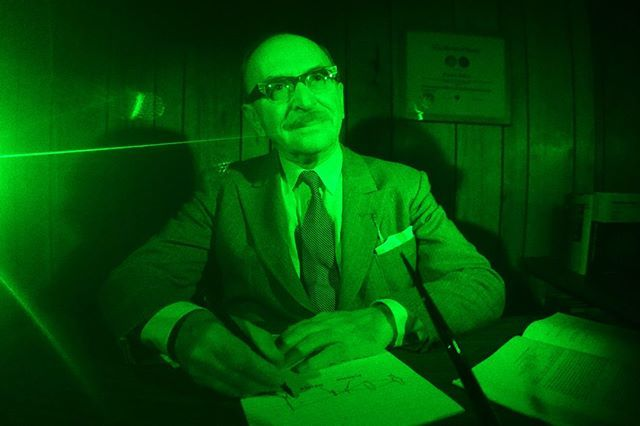
\includegraphics[width=0.6\textwidth]{Dennis-Gabor-Hologram-2.jpg}
    \caption{A photo of the holographic portrait of Dennis Gabor \cite{Lo2018}}\label{fig:Dennis-Gabor-Hologram-2}
\end{figure}

Holography, taking its name from the Greek word $o \lambda o \sigma $ (holos), meaning \textit{whole}, was first introduced in 1948 by Dennis Gabor \cite{Gabor1948}, originally named as \textit{wavefront reconstruction} \cite{Hecht2017}. It is a technology which generates 3D images via the diffraction of light. Similar to 2D photography, the earliest holography used a piece of film to record the diffraction pattern, which was then used to reconstruct the 3D field, as shown in \cref{fig:Dennis-Gabor-Hologram-2} which is a holographic recording of Dennis Gabor himself. After the invention of digital cameras, digital holography emerged. The limitation of both methods is that they require a physical object priori to record the hologram. In order to generate hologram for objects that do not physically exist, computer-generated holography (CGH) emerged where a hologram can be calculated through various algorithmic approaches and then displayed on a spatial light modulator (SLM) modulating the wavefront of a coherent light source in order to produce 3D reconstructions. Currently available SLM's can only modulate either phase or amplitude, so algorithms are needed to compute amplitude-only or phase-only holograms. The classic phase-retrieval algorithms include direct binary search \cite{Seldowitz1987}, simulated annealing \cite{Kirkpatrick1983} and Gerchberg-Saxton \cite{Gerchberg1972}. With the developments in modern numerical optimisation methods and increases in computational power, phase retrieval using numerical optimisation methods has also been found in the literature, such as the gradient descent \cite{Zhang2017, Liu2020} and its stochastic variations \cite{Chen2021, Choi2021, Kadis2022}. However, all the existing phase retrieval methods still have some fundamental issues, mainly their poor image quality and/or the heavy computation required, the solutions of which are the ultimate goals of this research.

This thesis therefore explores the development and optimisation of phase-only CGHs for holographic displays. The research investigates various phase retrieval algorithms and proposes novel methods to enhance the reconstruction quality and computational efficiency of CGHs, and then investigates the fundamental limits of discretised phase holograms from an information theory point of view. The thesis is structured as following.

Chapter 2 provides a comprehensive literature review, covering the fundamental theories of light, the principles of holography, and the evolution of CGH methods. The chapter reviews various phase retrieval algorithms, including the Naive, Direct Binary Search (DBS), Simulated Annealing (SA), Gerchberg-Saxton (GS), One-Step Phase Retrieval (OSPR), and Adaptive One-Step Phase Retrieval (AD-OSPR) algorithms and their adaptations for 3D CGHs, emphasizing the limitations of current algorithms and introducing the motivation for pursuing more advanced CGH techniques.

Chapter 3 proposes the Digital Pre-Distorted One-Step Phase Retrieval (DPD-OSPR) method. By experimentally evaluating the non-linearities in the holographic projection system and applying a digital pre-distortion (DPD) curve, significant improvements in reconstruction quality and reductions in mean squared error are demonstrated.

Chapter 4 introduces the optimisation of phase-only holograms using the Limited-memory Broyden-Fletcher-Goldfarb-Shanno (L-BFGS) optimisation algorithm, and then proposes the novel Target Image Phase Optimisation (TIPO) technique, which optimises the phase of the target image instead of the phase of the hologram. Then the multi-depth phase-only hologram optimisation for 3D targets is investigated, and a novel technique called Sequential Slicing (SS) is proposed, which evaluates the loss for a single slice of the 3D target at each iteration instead of a full evaluation on all slices, reducing computational time while maintaining overall quality and minimizing quality imbalances across all slices.

Chapter 5 extends the optimisation method on generating time-multiplexing binary-phase holograms, and proposes the novel Multi-Frame Holograms Batched Optimisation (MFHBO) technique. By optimising a batch of holograms for time multiplexing, which leverages the finite response time of human vision to average out noise, resulting in improved visual quality. The MFHBO algorithm shows a much better quality than the existing time-multiplexing hologram generation methods such as OSPR and AD-OSPR.

Chapter 6 investigates the information capacity of phase-only CGH. This chapter examines the effects of quantisation on hologram bit depth and their impact on reconstruction quality, and looks for the correlation between the entropy of the target image and the reconstruction error, providing insights into the fundamental limits of discretised CGH.

Chapter 7 marks the conclusion and lists potential further work that could be done.

%!TEX root = ../thesis.tex
%*******************************************************************************
%****************************** Literature Review Chapter **********************
%*******************************************************************************
\chapter{Literature Review} \label{sec:Literature Review}

\graphicspath{{Chapter_LR/Figs/}}
This chapter lays down the fundamental theories of optoelectronics and search algorithms, which are essential to the research outlined in the later chapters of this thesis.


\section{The Nature of Light}
\subsection{Wave-Particle Duality}
The problem of how light propagates has been troubling scientists for centuries. The journey began with Sir Isaac Newton, who advocated the particle theory of light in the 17th century. Newton proposed that light consists of particles, or `corpuscles', which explained phenomena such as reflection and refraction \cite{Newton1704}. In contrast, Christiaan Huygens, a contemporary of Newton, demonstrated that light behaves as a wave, as it is capable of diffraction and interference \cite{Huygens1690}.

\begin{figure}[H]
	\centering
	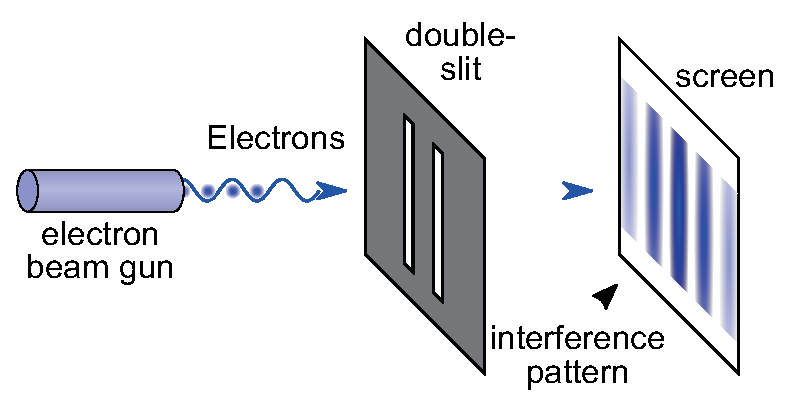
\includegraphics[width=0.7\textwidth]{Double-slit.eps}
	\caption{An illustration of the Young's Double-slit experiment \cite{Kalliauer2017}}
	\label{fig:Double-slit.eps}
\end{figure}

The wave theory gained significant support in the early 19th century through the experiments of Thomas Young. Young's double-slit experiment in 1801 provided clear evidence of the wave nature of light by showing that light passing through two slits creates an interference pattern on a screen \cite{Young1802}, as illustrated in \cref{fig:Double-slit.eps}. Augustin-Jean Fresnel further advanced the wave theory by developing a comprehensive mathematical framework to describe light as a wave, explaining phenomena such as polarization and the diffraction of light \cite{Fresnel1826}.

This understanding was further reinforced by James Clerk Maxwell in the mid-19th century. In 1864, James Clerk Maxwell organised a set of four equations describing the space and time dependence of the electromagnetic field, which are:
\begin{align}
  \nabla \times \mathbb{E} & = -\frac{\partial \mathbb{B}}{\partial t}             \label{eq:maxwell1} \\
  \nabla \times \mathbb{H} & = \mathbb{J} + \frac{\partial \mathbb{D}}{\partial t} \label{eq:maxwell2} \\
  \nabla \cdot \mathbb{D}  & = \rho                                                \label{eq:maxwell3} \\
  \nabla \cdot \mathbb{B}  & = 0 \label{eq:maxwell4}
\end{align}
where $\mathbb{D}$ is the electric flux density, $\mathbb{E}$ is the electric field intensity, $\mathbb{B}$ is the magnetic flux density, $\mathbb{H}$ is the magnetic field intensity, $\rho$ is the volume charge density, and $\mathbb{J}$ is the current density \cite{Daintith2009}.

And the relation between $\mathbb{D}$ and $\mathbb{E}$ and between $\mathbb{B}$ and $\mathbb{H}$ for linear materials are:
\begin{align}
  \mathbb{B} & = \mu \mathbb{H}      \\
  \mathbb{D} & = \epsilon \mathbb{E}
\end{align}
where $\mu$ is the magnetic permeability and $\epsilon$ is the dielectric permittivity of the material \cite{Wilkinson2017}.

Maxwell's equations unified electricity and magnetism into a single theory of electromagnetism, predicting that light is an electromagnetic wave that propagates through space \cite{Maxwell1865}.

Despite the success of the wave theory, it could not explain all light-related phenomena. The early 20th century brought a pivotal development with Albert Einstein's explanation of the photoelectric effect. In 1905, Einstein proposed that light also behaves as particles, or `quanta' (later called photons), which could eject electrons from a metal surface when light is shone upon it \cite{Einstein1905}. This particle nature of light was critical in explaining observations that wave theory alone could not address and earned Einstein the Nobel Prize in Physics in 1921.

These discoveries collectively revealed that light exhibits both wave and particle properties, depending on the experimental context. This wave-particle duality became a cornerstone of quantum mechanics, fundamentally altering human's understanding of the nature of light. Although to date, it is still not yet known what light exactly is, it is now known how light behaves.

\subsection{Wave Equation}
To mathematically describe the propagation of light in free space (i.e. in absence of free charge), the Maxwell equations in \cref{eq:maxwell1} - \cref{eq:maxwell4} can be simplified as:
\begin{align}
  \nabla \times \mathbb{E}         & = -\mu \frac{\partial \mathbb{H}}{\partial t}     \label{eq:simplified_maxwell1} \\
  \nabla \times \mathbb{H}         & = \epsilon \frac{\partial \mathbb{E}}{\partial t} \label{eq:simplified_maxwell2} \\
  \nabla \cdot \epsilon \mathbb{E} & = 0                                               \label{eq:simplified_maxwell3} \\
  \nabla \cdot \mu \mathbb{H}      & = 0 \label{eq:simplified_maxwell4}
\end{align}

Taking the curl on both the left and right hand sides of \cref{eq:simplified_maxwell1}, and using the vector identity of $\nabla \times (\nabla \times \textbf{u}) = \nabla(\nabla \cdot \textbf{u}) - \nabla^2 \textbf{u}$, we get:
\begin{align}
  \nabla \times (\nabla \times \mathbb{E})               & = -\nabla \times (\mu \frac{\partial \mathbb{H}}{\partial t}) \label{eq:wave_equation_derivation1} \\
  \nabla (\nabla \cdot \mathbb{E}) - \nabla^2 \mathbb{E} & = -\frac{\partial}{\partial t} \nabla \times (\mu \mathbb{H}) \label{eq:wave_equation_derivation2}
\end{align}

Then, by substituting \cref{eq:simplified_maxwell2} and \cref{eq:simplified_maxwell3} in, \cref{eq:wave_equation_derivation2} becomes:
\begin{equation}
  -\nabla^2 \mathbb{E} = -\frac{\partial}{\partial t} (\mu \epsilon \frac{\partial \mathbb{E}}{\partial t}) \label{eq:wave_equation_derivation3}
\end{equation}

Hence, we have a generic form of wave equation, relating the space and time domain relation of electromagnetic waves propagating in free space:
\begin{equation}
  \nabla^2 \mathbb{E} = \mu \epsilon \frac{\partial^2 \mathbb{E}}{\partial t^2} \label{eq:wave_equation}
\end{equation}

A valid solution to \cref{eq:wave_equation} is:
\begin{equation}
  \mathbb{E} = \mathbb{E}_0 e^{j(\omega t - k r)} \label{eq:wave_equation_solution}
\end{equation}
where $\omega$ is the angular velocity of the wave, $t$ is time, $r$ is the propagation distance and $k$ is called the wave number ($k=\frac{2\pi}{\lambda}$, where $\lambda$ is the wavelength). From \cref{eq:wave_equation_solution} we can see that the propagation of light in free space is essentially a phase shift. This suggests that, if we have a coherent light source and a device to manipulate light (called SLM, further explained in \cref{sec:SLM}), we can produce an interference pattern reconstructing the target field we desire, and such method is called holographic projection.


\newpage
\section{Fundamentals of Holography}
Holography is a technology that can fully reconstruct the wavefront of 3D objects, which is usually achieved by modulating a coherent light source. This section explains what a coherent light source is and how it is modulated and diffracted.

\subsection{Light Source} \label{sec:Light Source}

The mechanism of holographic projection is to control the propagation of light in a way that, after diffraction, reconstructs a wavefront that matches the target field. We usually prefer to start from a coherent light source rather than a random one which will be a lot more difficult or even impossible to analyse and predict the interference pattern.

\begin{figure}[H]
	\centering
	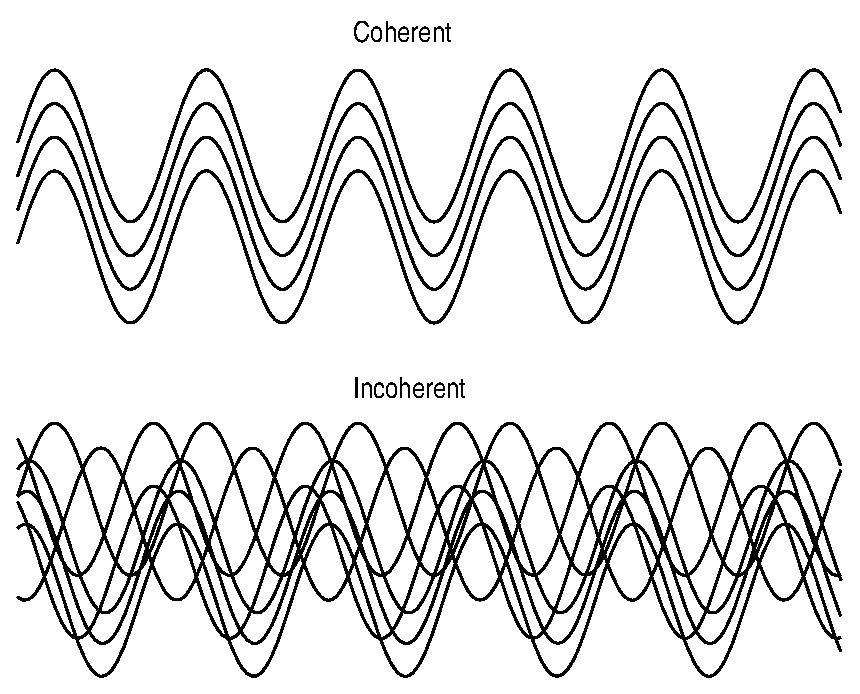
\includegraphics[width=0.7\textwidth]{coherent-vs-incoherent.eps}
	\caption{Coherent v.s. incoherent light}
	\label{fig:coherent-vs-incoherent.eps}
\end{figure}

The coherence of light refers to the property of light waves where the phase relationship between the waves is consistent over time and space, corresponding to temporal and spatial coherence:
\begin{itemize}
  \item \textbf{Temporal coherence:} Temporal coherence describes the correlation between the phases of a light wave at different points along its propagation direction. It indicates how monochromatic (i.e. single-frequency) a light source is.
  \item \textbf{Spatial coherence:} Spatial coherence describes the correlation between the phases of a light wave at different points across the wavefront, perpendicular to the direction of propagation. It indicates the uniformity of the phase across the wavefront, as illustrated in \cref{fig:coherent-vs-incoherent.eps}. High spatial coherence means that the light waves across different points on the wavefront are in phase.
\end{itemize}

\begin{figure}[H]
	\centering
	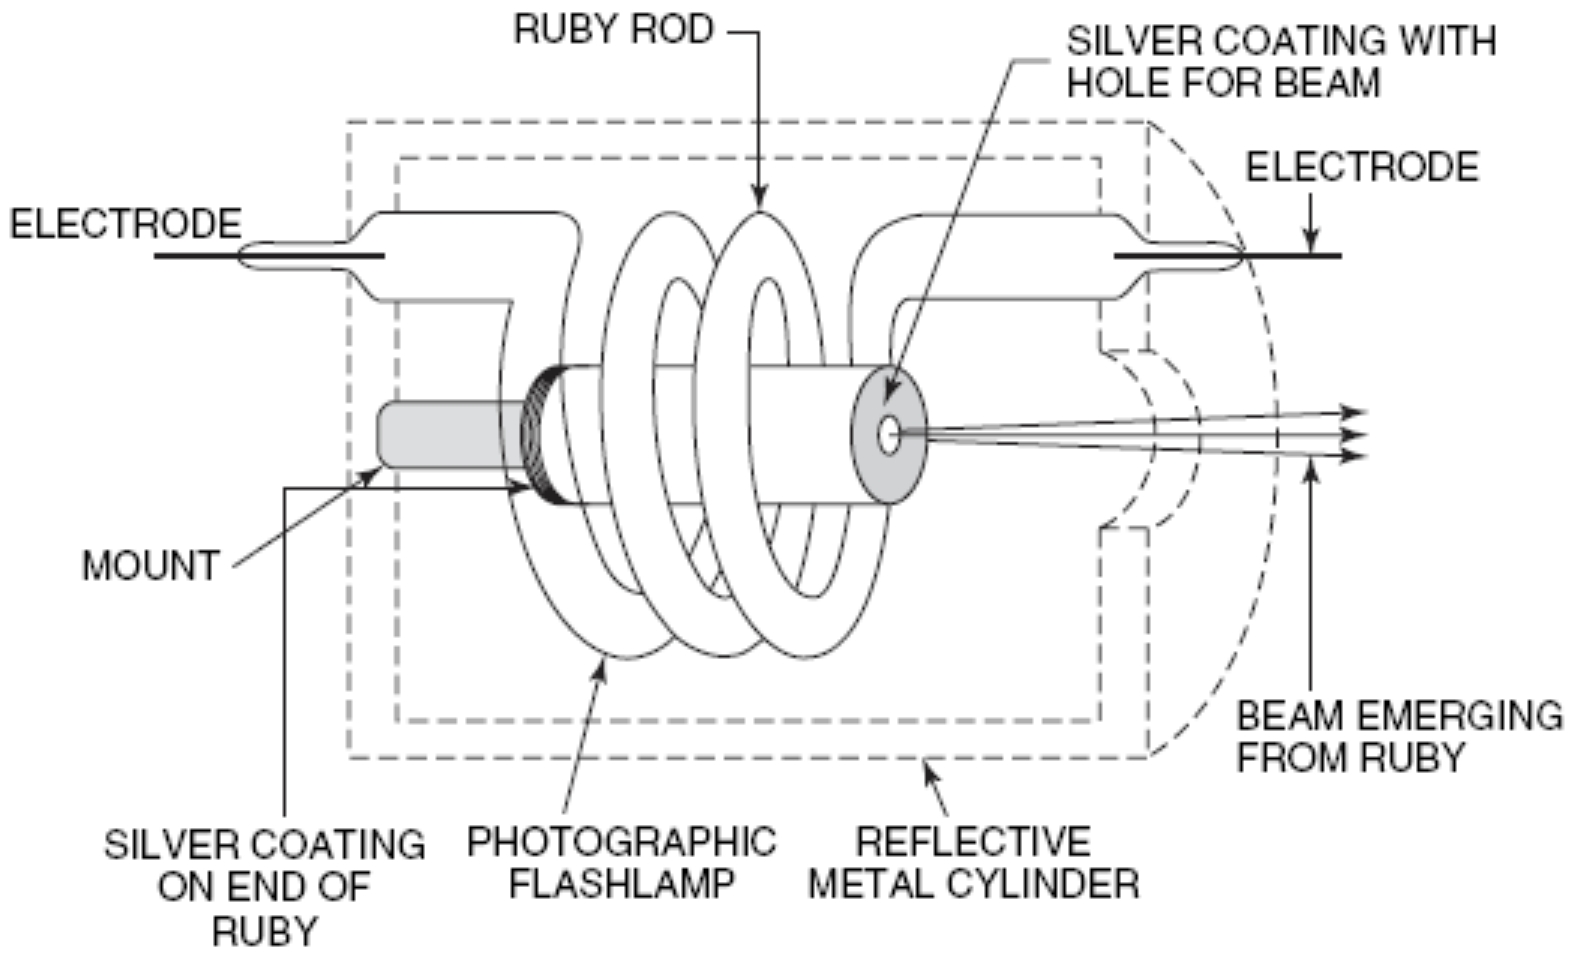
\includegraphics[width=0.9\textwidth]{first_laser.jpg}
	\caption{Structure of the first laser \cite{Hecht2008}}
	\label{fig:first_laser}
\end{figure}

The most common coherent light source is Laser, which stands for \textit{\textbf{L}ight \textbf{A}mplification by the \textbf{S}timulated \textbf{E}mission of \textbf{R}adiation}. It was first invented by Theodore Maiman in 1959, with the structure shown in \cref{fig:first_laser} \cite{Hecht2008, Gordon1959, Cartlidge2007}. It differs from other sources of light in that it emits coherent light, which is suitable for holographic projection. However, the coherent and monochromatic property of laser also has a side effect of speckle noise in the reconstructed image \cite{John1966}, which is one of the major problems affecting the image quality of holographic projections and has seen lots of efforts to cope with it in the literature \cite{Cable2004,Stangner2017,Deng2021,Hands2022}.


\subsection{Diffraction} \label{sec:Diffraction}

This section delves into how light interacts with apertures, leading to diffractions. Understanding diffraction is essential for holography, as it explains how light can be manipulated to reconstruct three-dimensional light fields. The principles of diffraction and interference underpin the essential process of holographic projection, making it possible to accurately recreate complex wavefronts and achieve true 3D visualization.

\begin{figure}[H]
  \centering
  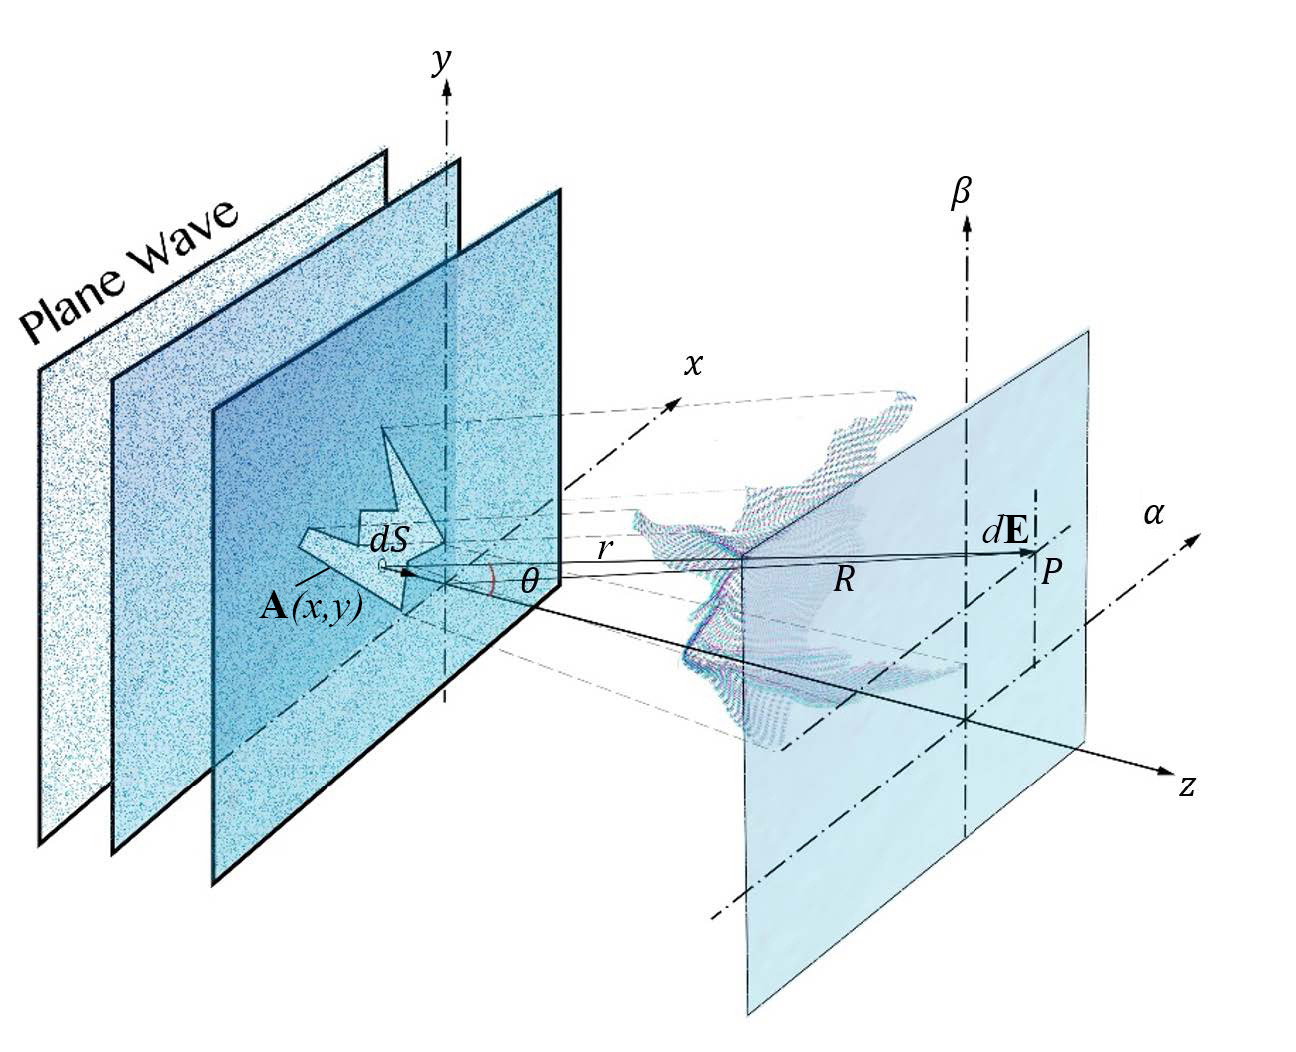
\includegraphics[width=0.8\textwidth]{diffraction_coordinate_definition.jpg}
  \caption{Diffraction geometry}\label{fig:diffraction_coordinate_definition}
\end{figure}

To model how light diffracts through a 2D aperture, we first set up a coordinate system as shown in \cref{fig:diffraction_coordinate_definition}, where the aperture is denoted by $A(x, y)$ and the diffracted field is denoted by $E(\alpha, \beta, z)$. $R$ defines the distance between point $P$ and the origin of the aperture ($(x,y)=(0,0)$), $r$ defines the distance between point $P$ and a point on the aperture, and $\theta$ defines the angle $r$ from the $z$-axis. Then by trigonometry we can have the following identities:
\begin{align}
  cos(\theta) & = \frac{z}{r}                      \label{eq:trignometry-theta} \\
  R^2         & = \alpha ^2 + \beta ^2 + z^2       \label{eq:trignometry-R} \\
  r^2         & = (\alpha-x)^2 + (\beta-y)^2 + z^2 \label{eq:trignometry-r}
\end{align}

\begin{figure}[H]
  \centering
  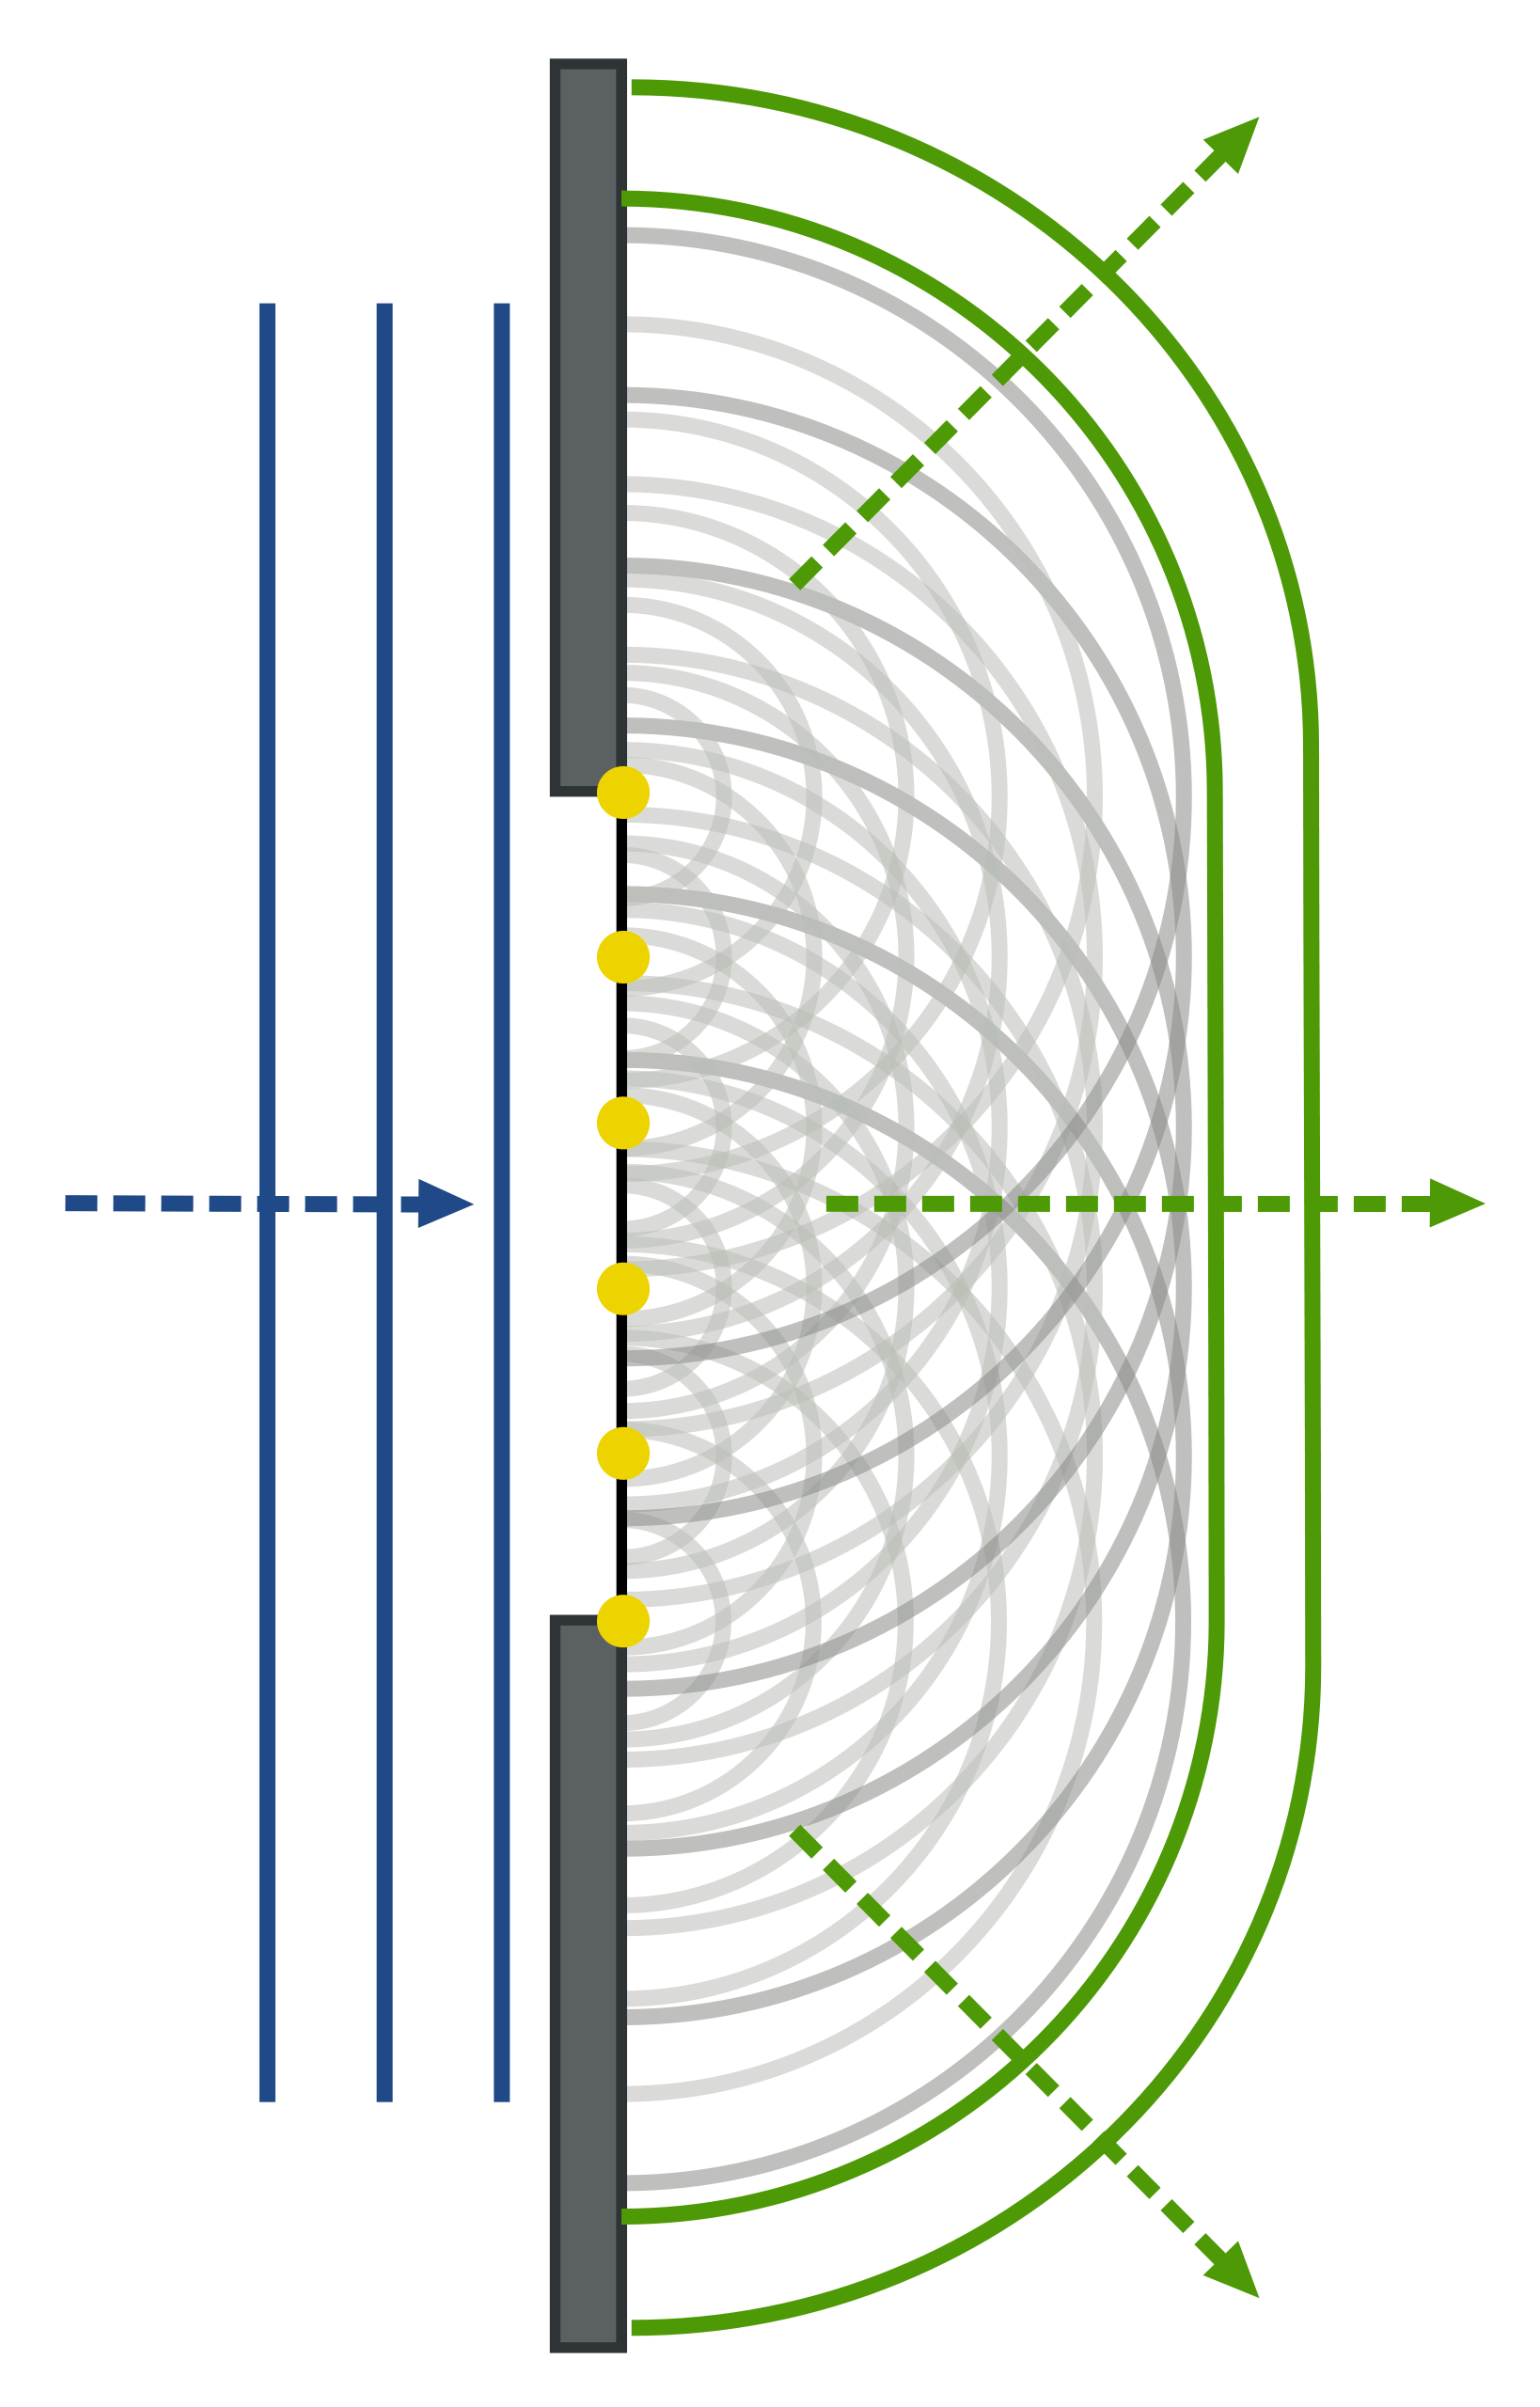
\includegraphics[width=0.3\textwidth]{huygens_wavelets_principle.png}
  \caption{Huygens-Fresnel wavelet principle \cite{Nordmann2007}}\label{fig:huygens_wavelets_principle}
\end{figure}

The Huygens-Fresnel principle states that every point on a wavefront is itself the source of outgoing secondary spherical wavelets, which can be expressed mathematically as follows when $r\gg \lambda$ \cite{Goodman2017}:
\begin{equation}
  E(\alpha, \beta, z) = \frac{1}{j\lambda} \iint A(x,y)\frac{e^{jkr}}{r} cos(\theta) dxdy \label{eq:huygens-fresnel-principle}
\end{equation}

Applying the identities in \cref{eq:trignometry-theta} - \cref{eq:trignometry-r},  \cref{eq:huygens-fresnel-principle} becomes:
\begin{align}
  E(\alpha, \beta, z) & = \frac{z}{j\lambda} \iint A(x,y)\frac{e^{jkr}}{r^2} dxdy                    \label{eq:huygens-fresnel-principle-substituded-cos}                                                      \\
                      & = \frac{z}{j\lambda} \iint A(x,y)\frac{e^{jk\sqrt{(\alpha-x)^2 + (\beta-y)^2 + z^2}}}{(\alpha-x)^2 + (\beta-y)^2 + z^2} dxdy \label{eq:huygens-fresnel-principle-substituded-r-square}
\end{align}

Unfortunately, \cref{eq:huygens-fresnel-principle-substituded-r-square} cannot be solved analytically except for few specific aperture functions $A(x,y)$, so we have to make some approximations in order to solve for arbitrary $A(x,y)$, the common methods are \textit{Fresnel} and \textit{Fraunhofer} approximations for regions depicted in \cref{fig:fresnel_fraunhofer_approximations}.

\begin{figure}[H]
  \centering
  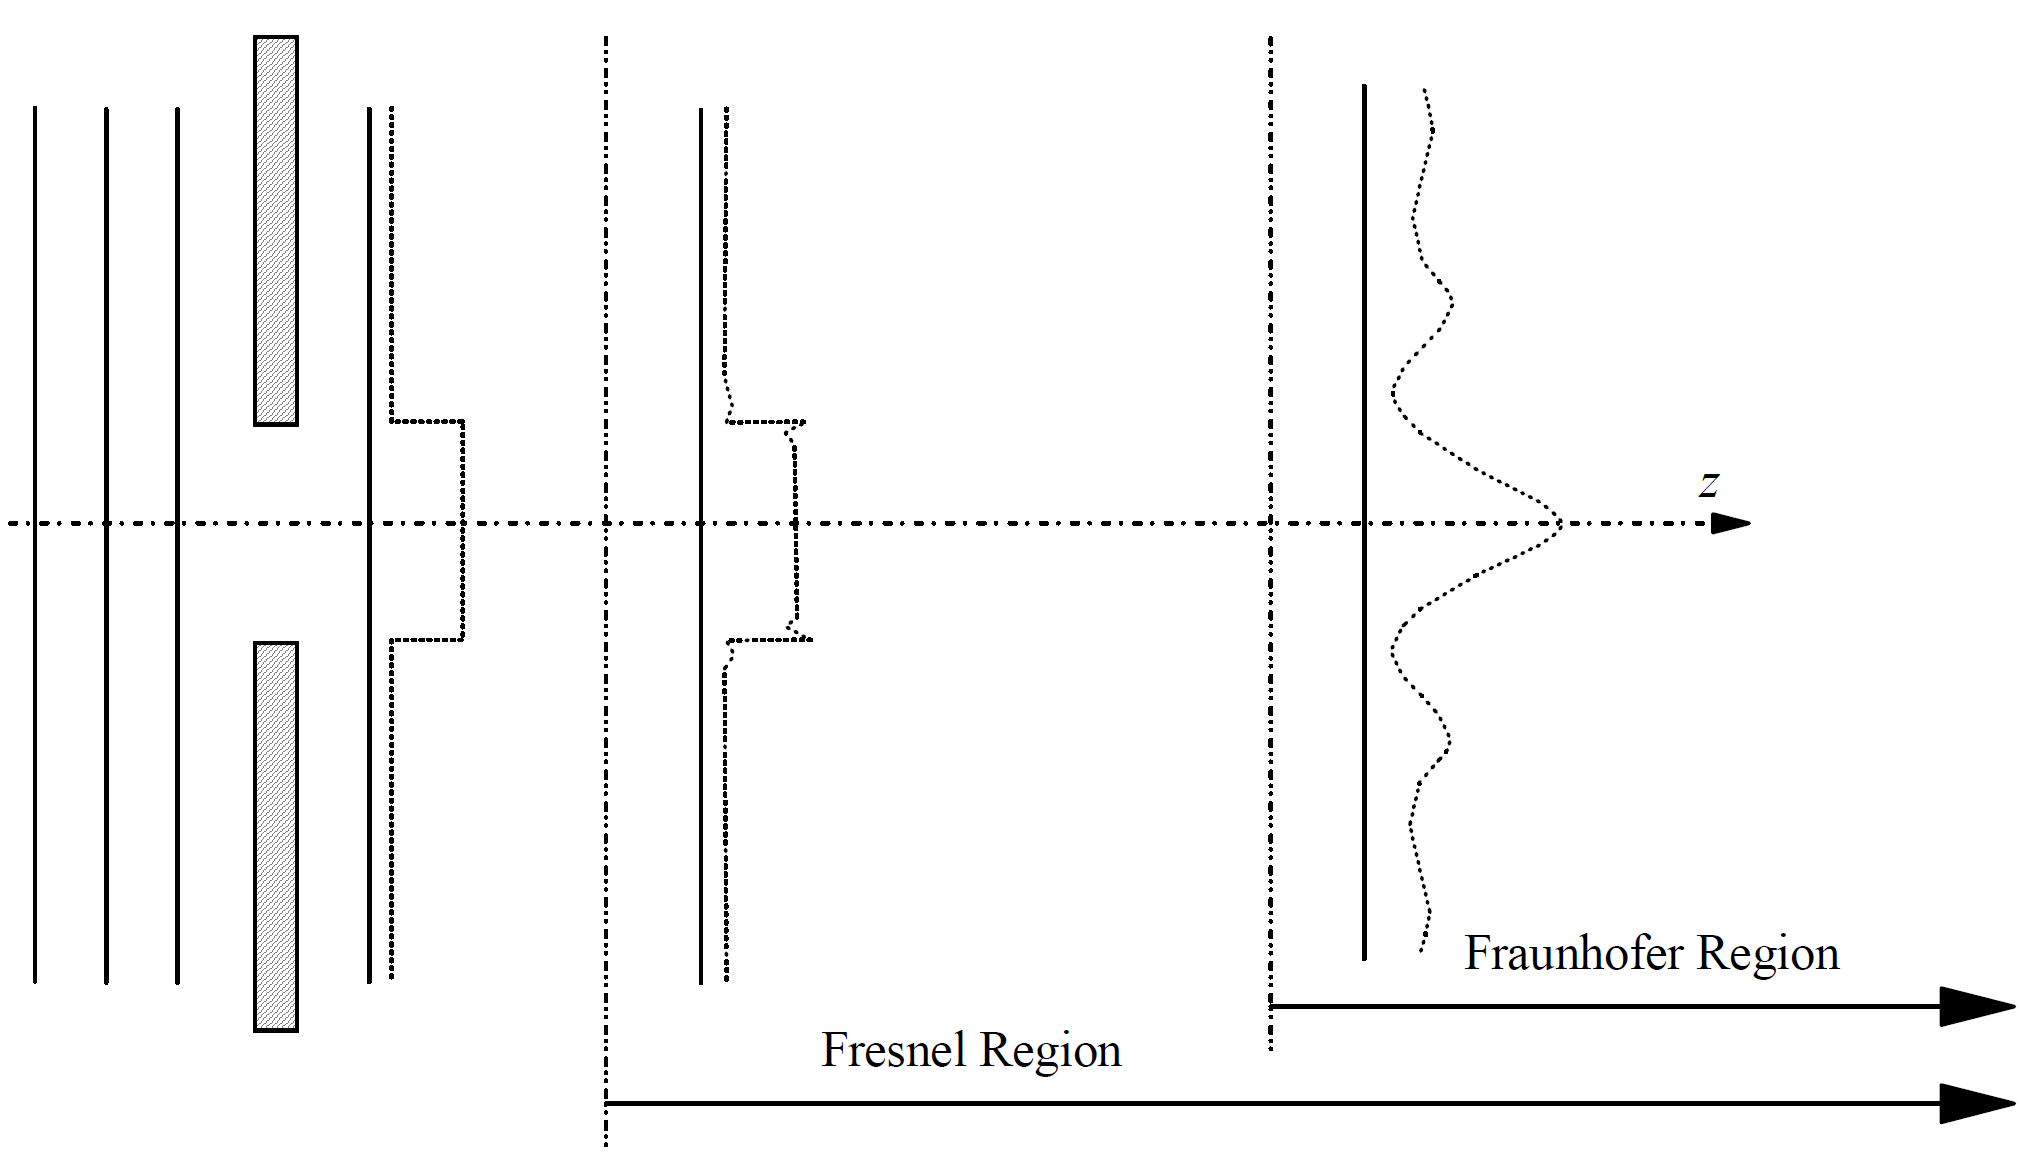
\includegraphics[width=0.9\textwidth]{fresnel_fraunhofer_approximations.png}
  \caption{Fresnel and Fraunhofer region \cite{Wilkinson2019}}\label{fig:fresnel_fraunhofer_approximations}
\end{figure}


\subsubsection{Fresnel Approximation}
\begin{equation}
  \sqrt{1+d} = 1 + \frac{1}{2}d - \frac{1}{8}d^2 + \cdots \label{eq:binomial-expension}
\end{equation}
Fresnel approximation replaces expressions for spherical waves by quadratic-phase exponentials, using the binomial expansion of the square root (given in \cref{eq:binomial-expension}) to approximate $r$ in \cref{eq:huygens-fresnel-principle-substituded-cos} \cite{Goodman2017}.

Retaining only the first two terms of the expansion gives:
\begin{align}
  r & = \sqrt{(\alpha-x)^2 + (\beta-y)^2 + z^2}                                                                                                              \\
    & = z \sqrt{1 + \left( \frac{\alpha-x}{z} \right)^2 + \left(\frac{\beta-y}{z}\right)^2}                                                                  \\
    & \approx z \left[ 1 + \frac{1}{2} \left( \frac{\alpha-x}{z} \right)^2 + \frac{1}{2} \left(\frac{\beta-y}{z}\right)^2 \right] \label{eq:r-approximation}
\end{align}

For the $r^2$ in the denominator of \cref{eq:huygens-fresnel-principle-substituded-cos}, the error introduced by dropping all terms but $z$ is generally acceptably small (i.e. $r^2\approx z^2$), and for the $r$ appearing in the exponent in the numerator of \cref{eq:huygens-fresnel-principle-substituded-cos}, errors are much more critical \cite{Goodman2017}. So, by substituting \cref{eq:r-approximation} for the $r$ in the numerator of \cref{eq:huygens-fresnel-principle-substituded-cos} and substituting $z$ for the $r$ in the denominator, we have:
\begin{align}
  E(\alpha, \beta, z) & \approx \frac{z}{j\lambda} \iint A(x,y)\frac{e^{jkz \left[ 1 + \frac{1}{2} \left( \frac{\alpha-x}{z} \right)^2 + \frac{1}{2} \left(\frac{\beta-y}{z}\right)^2 \right]}}{z^2} dxdy \\
                      & = \frac{e^{jkz}}{j\lambda z} e^{j\frac{k}{2z}(\alpha^2+\beta^2)} \iint \left\{A(x,y)e^{j\frac{k}{2z}(x^2+y^2)}\right\}e^{-j\frac{2\pi}{\lambda z}(\alpha x+\beta y)}dxdy    \\
                      & = \frac{e^{jkz}}{j\lambda z} e^{j\frac{k}{2z}(\alpha^2+\beta^2)} \mathcal{F} \left\{A(x,y)e^{j\frac{k}{2z}(x^2+y^2)}\right\}
\end{align}
where $\mathcal{F}$ is the Fourier Transform. Such method of including Fourier Transform (FT) in the study of optics is also named `Fourier Optics'.

Now we have a more simple and solvable expression than \cref{eq:huygens-fresnel-principle-substituded-r-square}. And also, as we are only interested in the scaling of relative points at $P$ with respect to each other, so it is safe to normalise the multiplier term before the Fourier Transform to 1 \cite{Wilkinson2019}. So we can express the diffraction pattern in Fresnel region as:
\begin{equation}
  E_{Fresnel\ region}(\alpha, \beta, z) = \mathcal{F} \left\{A(x,y)e^{j\frac{k}{2z}(x^2+y^2)}\right\} \label{eq:fresnel-diffraction}
\end{equation}


\subsubsection{Fraunhofer Approximation}
Fraunhofer diffraction is a form of diffraction in which the distance between the light source and the receiving screen are in effect at infinite, so that the wave fronts can be treated as planar rather than spherical \cite{Daintith2009}. Fraunhofer approximation is very stringent, it assumes that the distance between the light source and the receiving screen are in effect at infinite:
\begin{equation}
  z\gg \frac{k(x^2+y^2)_{max}}{2}
\end{equation}

so that the wave fronts can be treated as planar rather than spherical \cite{Daintith2009}, then the $e^{j\frac{k}{2z}(x^2+y^2)}$ term tends to $1$, and \cref{eq:fresnel-diffraction} becomes:
\begin{equation}
  E_{Fraunhofer\ region}(\alpha, \beta) = \mathcal{F} \left\{A(x,y)\right\}
\end{equation}

which suggests that the far field pattern is simply the Fourier Transform of the aperture function.


\subsection{Spatial Light Modulator (SLM)} \label{sec:SLM}
SLMs are critical components in computer-generated holography (CGH). SLM is a device used to control the amplitude or phase of light waves in a spatially varying manner. SLMs typically consist of a two-dimensional(2D) array of pixels, each of which can modulate the light either passing through or reflected from it. These pixels are usually addressed by electronic signals, allowing precise manipulation of the light wavefront.

\begin{figure}[H]
  \centering
  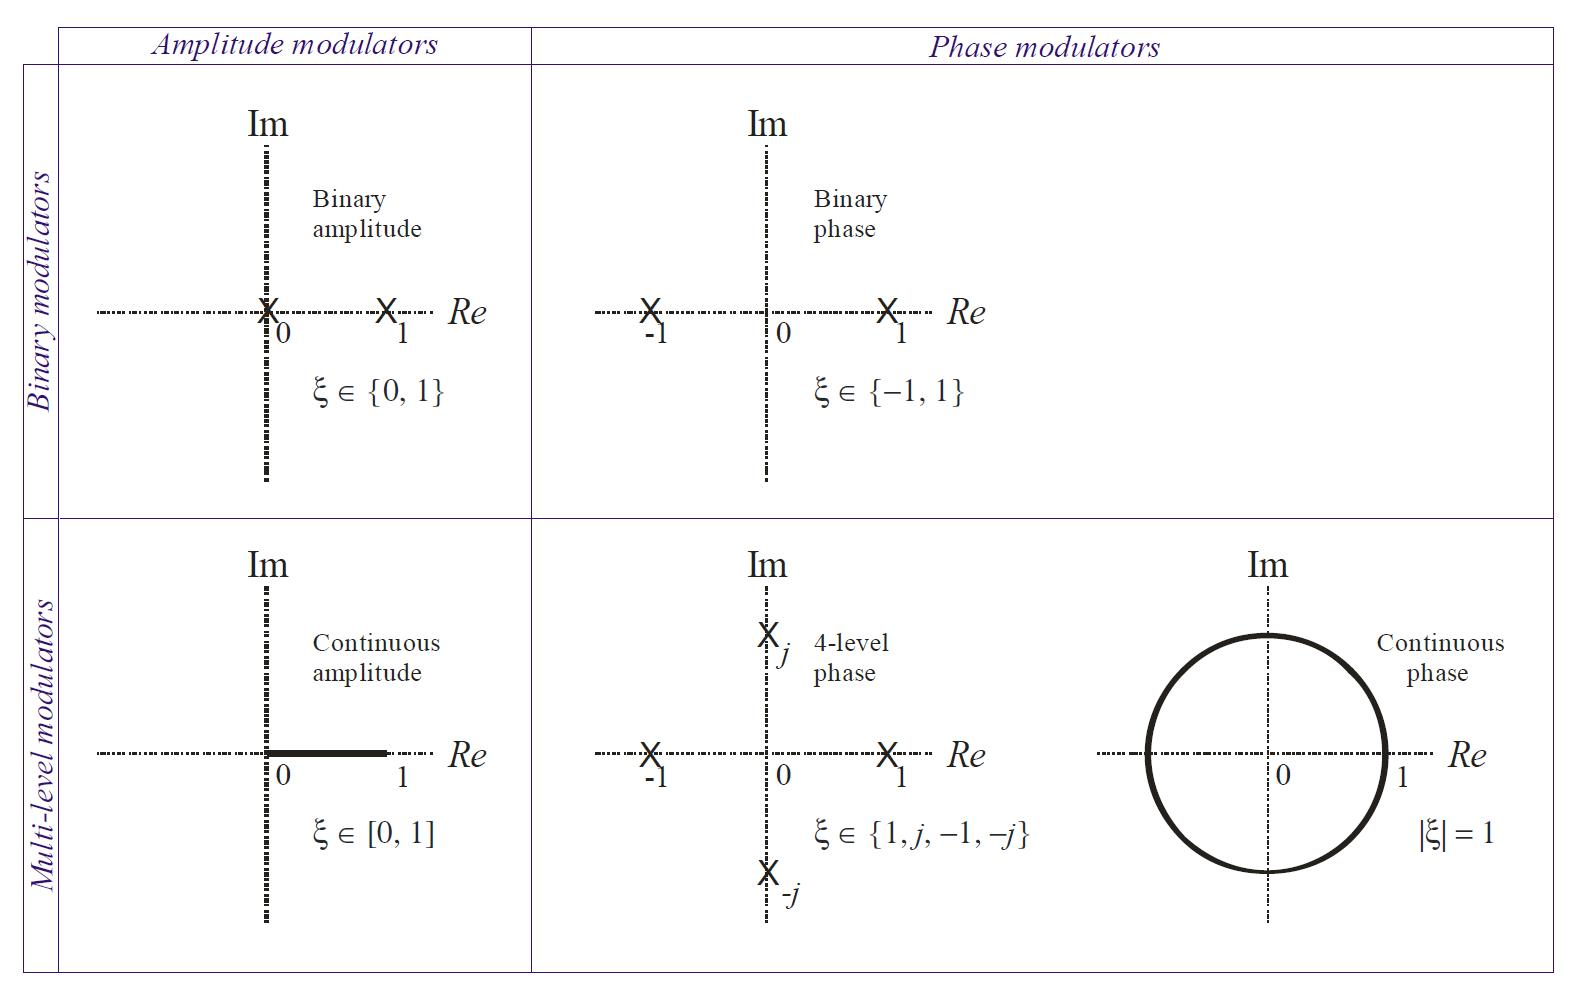
\includegraphics[width=1.0\textwidth]{modulation_loci.jpg}
  \caption{Modulation loci in the complex plane \cite{Cable2006}} \label{fig:modulation_loci}
\end{figure}

The modulation can be achieved through various mechanisms, such as liquid crystal SLMs(LC-SLM), magneto-optic SLMs, deformable mirror SLMs, multiple-quantum-well SLMs, or acousto-optic Bragg cells \cite{Goodman2017}, which all fall into the four modulation categories, as illustrated in \cref{fig:modulation_loci} \cite{Cable2006}. The four modulation schemes are:

\begin{itemize}
  \item \textbf{Multi-level Amplitude} modulators can modulate each pixel from zero transmission (0) to full transmission (1), either continuously or in discrete steps. (e.g. nematic liquid crystal display \cite{Schadt1971}, found for example in laptops and many conventional video projectors)
  \item \textbf{Binary Amplitude} modulators can switch each pixel to zero transmission (0) or full transmission (1), but nothing in between. (e.g. deformable mirror device \cite{Pape1983}, ferroelectric liquid crystal display \cite{Johnson1993}, both used in high-end video projectors)
  \item \textbf{Multi-level Phase} modulators can modulate the phase shift imparted by each pixel from 0 to 2$\pi$ radians, either continuously or in discrete steps. (e.g. Nematic liquid crystal devices \cite{Lee2004})
  \item \textbf{Binary Phase} modulators can switch each pixel for a phase shift of either 0 or $\pi$ radians. (e.g. Ferroelectric liquid crystal displays \cite{Broomfield1992})
\end{itemize}

Among the four modulation schemes, phase modulations are of higher interests for the purpose of holography, because amplitude modulators, either multi-level or binary, blocks light at the SLM, causing waste of energy, leading to poorer energy efficiency. And also, amplitude modulations always have a zero-order (forming a central bright spot), because the average amplitude is always between 0 and 1; on contrary, phase modulation can suppress the zero-order by designing the hologram to have zero average.

As there is no complex modulator available yet, we need algorithms to generate phase-only holograms, such process is called phase retrieval. There are currently many algorithms for such purpose, which will be discussed in \cref{sec:cgh}.

\subsubsection{Rotational symmetries in the binary phase modulation} \label{sec:Rotational symmetries in the binary phase modulation}

The spatial light modulator (SLM) used in this thesis is a binary phase modulator. As the binary phase modulation is purely real (i.e. it's only switching between $0^\circ$ and $180^\circ$, corresponding to 1 and -1 values of $A^*(x,y)$), the complex conjugate $A^*(x,y)$ is the same as $A(x,y)$:
\begin{equation} \label{eq:AequalsAstar}
  A^*(x,y) = A(x,y)
\end{equation}
because the Fourier transform of $A^*(x,y)$ is the same as the Fourier transform of $A(x,y)$
\begin{equation} \label{eq:AAstar}
  E(-\alpha, -\beta)=\mathcal{F}[A^*(x,y)]=\mathcal{F}[A(x,y)]=E(\alpha, \beta)
\end{equation}
So, at the Fraunhofer region, there is no distinction between the desired image and its $180^\circ$ rotation in the replay field, causing a symmetrical conjugate image rotated $180^\circ$ from the target image.

\begin{figure}[H]
  \centering
  \begin{subfigure}[t]{0.45\textwidth}
    \centering
    
\includegraphics[width=\textwidth]{10_step_target.jpg}
    \caption{Target image}
    \label{fig:10_step_target}
  \end{subfigure}
  \hfill
  \begin{subfigure}[t]{0.45\textwidth}
    \centering
    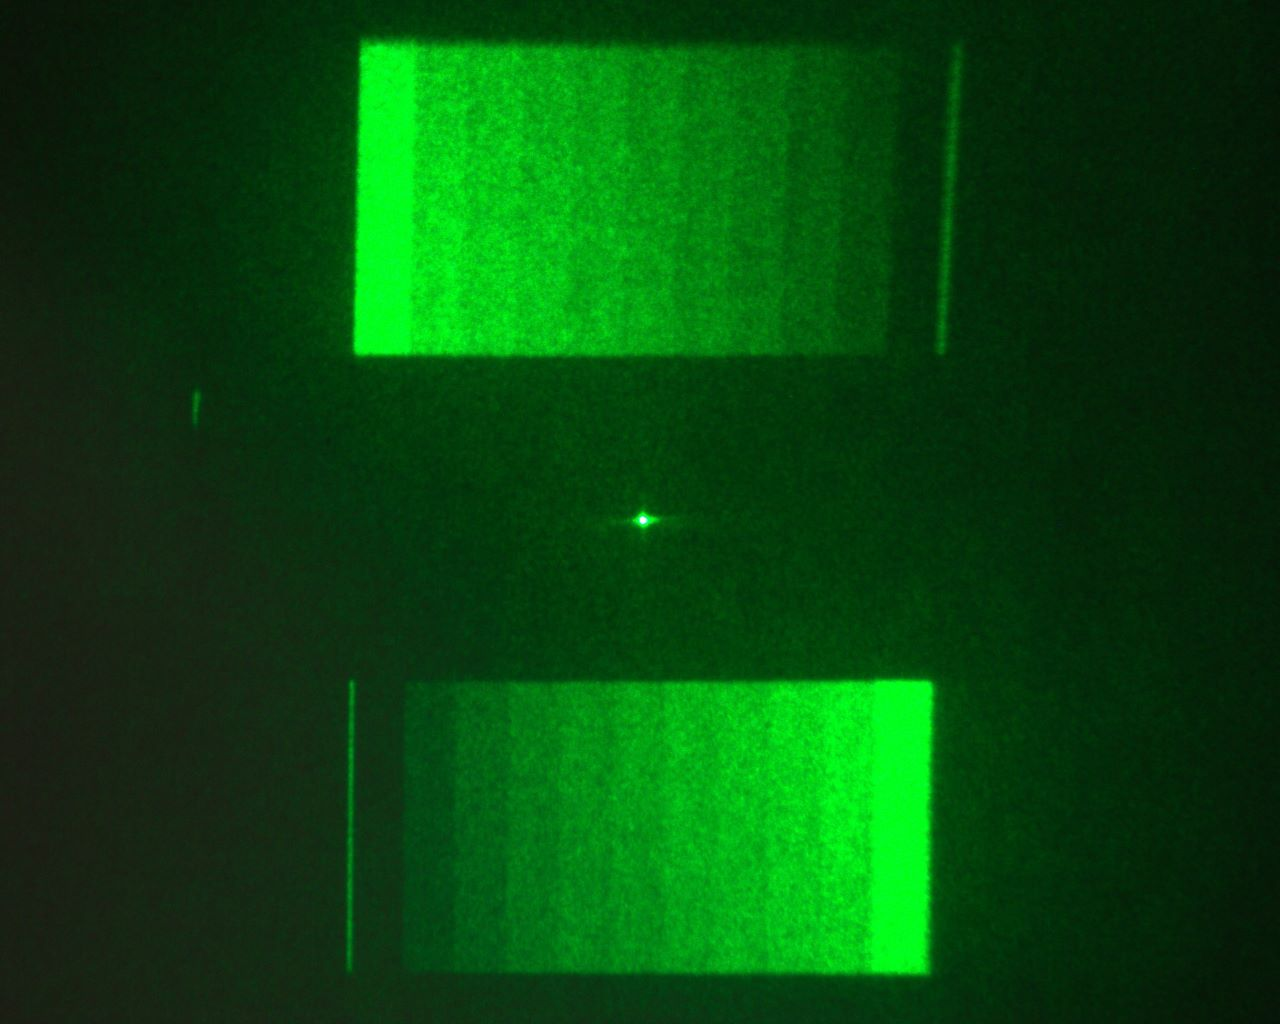
\includegraphics[width=\textwidth]{binary_phase_SLM_symmetry.jpg}
    \caption{Projection result}
    \label{fig:binary_phase_SLM_symmetry}
  \end{subfigure}

  \caption{Rotational symmetry in the projection result using the binary phase SLM}
  \label{fig:Rotational symmetry Binary SLM}
\end{figure}

To demonstrate such phenomena, the example target image shown in \cref{fig:10_step_target} ran through the binary-phase hologram generation algorithm called one-step phase-retrieval (OSPR), which will be explained in detail in \cref{sec:One Step Phase Retrieval (OSPR) Algorithm}, and the projection output is shown in \cref{fig:binary_phase_SLM_symmetry}. The simplest workaround for this issue is to use only half of the reconstruction field, like the target image in \cref{fig:10_step_target}. However, the side effect of this workaround is that half of the energy will be wasted, leading to higher power consumption and heat dissipation.



\newpage
\section{Computer-Generated Holography (CGH)}\label{sec:cgh}
Different from the traditional analogue optical holography and digital holography which both need a physically existing object to record the hologram, CGH is a method to use computer algorithms to generate holograms without the need for the physical target object. Ideally, holograms can be simply computed using the inverse Fourier Transform, using the inverse functions of \cref{eq:fresnel-diffraction} and \cref{eq:fraunhofer-diffraction} derived in \cref{sec:Diffraction}. The inverse Fourier Transforms on most targets will end up with results in complex numbers; however, as mentioned in \cref{sec:SLM}, currently available SLMs cannot achieve complex modulation yet. Therefore, computer algorithms are needed to compute either phase-only or amplitude-only holograms, among which the former is preferred, as explained in \cref{sec:SLM}.

This section reviews the existing methods in the literature for calculating phase-only holograms. The phase-only hologram is labelled as $H$, so that it differs from the previous notation of $A$ for complex-valued hologram apertures. And the propagation function is unified as $\mathcal{P}$, which can be either the Fraunhofer propagation equation in \cref{eq:fresnel-diffraction} or the Fresnel propagation equation in \cref{eq:fraunhofer-diffraction} depending on the distance of the target field. Lastly, $R$ denotes the reconstruction from the hologram, which is the amplitude of the result from $\mathcal{P}$.

\begin{figure}[H]
  \centering
  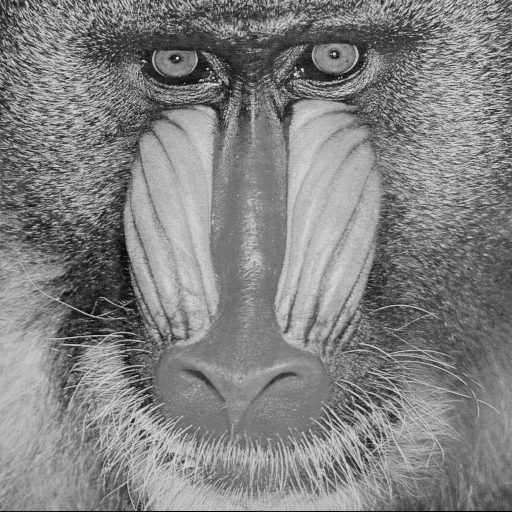
\includegraphics[width=0.3\textwidth]{mandrill.png}
  \caption{Sample target image of a mandrill ($T$) \cite{MANDRILL_REF}}\label{fig:mandrill.png}
\end{figure}

A sample image of a mandrill (shown in \cref{fig:mandrill.png}) is chosen from the University of Southern California Signal and Image Processing Institute (USC-SIPI) Image Database \cite{MANDRILL_REF} to test and compare the classical phase retrieval algorithms in the literature. As the square of the amplitude, also known as the `intensity' of light, is the only visible component with human eyes \cite{Huang2024}, the diffracted electric field's amplitude ($\vert E \vert$) will be targeted to match the square root of $T$.


\subsection{Naive Method}\label{sec:Naive algorithm}
The simplest method to get a phase-only hologram $H$ is by directly extracting the phase of the reverse propagation from the target field, discarding the amplitude component (e.g. for Fraunhofer propagation, $H$ will simply be the phase of the inverse Fourier transform $\mathcal{F} ^{-1}$ of the target field). This method is named as `Naive' method in this thesis for its simplicity. The pseudocode of the Naive method is shown in \cref{alg:Naive algorithm} below:
\begin{algorithm}[H]
  \caption{Naive method}\label{alg:Naive algorithm}
  \textbf{Input:} Target image $T$, Propagation function $\mathcal{P}$ (e.g. Fresnel or Fraunhofer propagation)\\
  \textbf{Output:} Phase hologram $H$ and its reconstruction intensity $R$
  \begin{algorithmic}
    \State $E \gets \sqrt{T}$
    \State $A \gets \mathcal{P}^{-1}[E]$
    \State $H \gets \angle A$
    \State $R \gets \vert \mathcal{P}[e^{jH}] \vert ^2 $
  \end{algorithmic}
\end{algorithm}
where $j = \sqrt{-1} $, the $\angle$ sign means phase extraction (i.e. arguments of complex numbers element-wise in the matrix), and $e^{jH}$ converts the angles back to complex numbers. All exponentials, modulus and square-root operators are carried out in an element-wise manner, so that the dimensions of $T$, $A$, $H$, $R$ and $E$ are all the same.

The Naive method (described in \cref{alg:Naive algorithm}) was then implemented in MATLAB and ran on the sample target image shown in \cref{fig:mandrill.png}, with the distance set to infinity (i.e. in the Fraunhofer region using the propagation formula \cref{eq:fraunhofer-diffraction}). The results are shown in \cref{fig:Naive algorithm output} below:

\begin{figure}[H]
  \centering
  \begin{subfigure}[t]{0.3\textwidth}
    \centering
    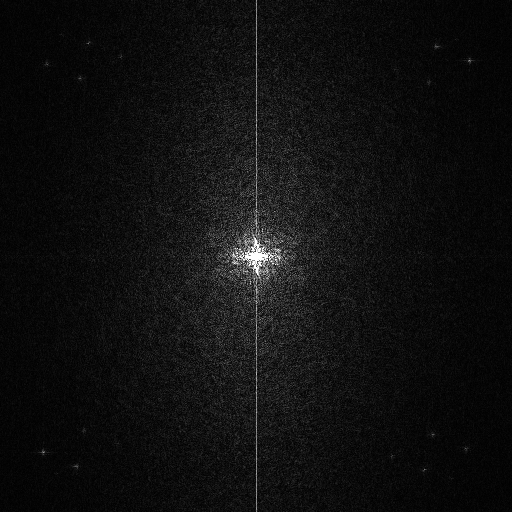
\includegraphics[width=\textwidth]{Naive_discarded_amplitude.png}
    \caption{Discarded amplitude ($\vert A\vert$)}
    \label{fig:Naive_discarded_amplitude}
  \end{subfigure}
  \hfill
  \begin{subfigure}[t]{0.3\textwidth}
    \centering
    
\includegraphics[width=\textwidth]{Naive_output_holo.png}
    \caption{Phase Hologram ($H$)}
    \label{fig:Naive_output_holo}
  \end{subfigure}
  \hfill
  \begin{subfigure}[t]{0.3\textwidth}
    \centering
    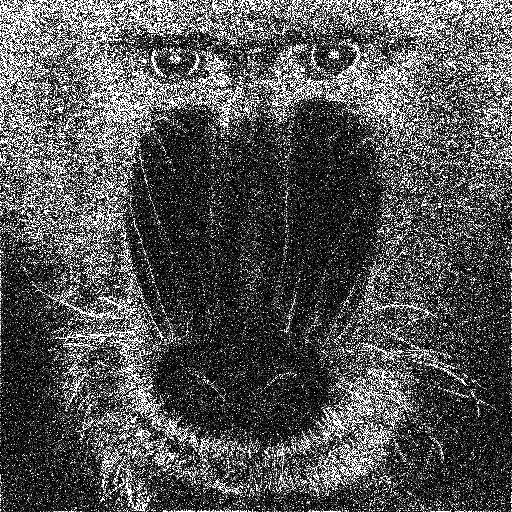
\includegraphics[width=\textwidth]{Naive_output_recon.png}
    \caption{Reconstruction ($R$)}
    \label{fig:Naive_output_recon}
  \end{subfigure}
  \caption{Naive method output}
  \label{fig:Naive algorithm output}
\end{figure}

After taking the inverse Fourier Transform, the amplitude and the phase of $A$ are shown in \cref{fig:Naive_discarded_amplitude} and \cref{fig:Naive_output_holo} respectively. The next step then discards the amplitude component (\cref{fig:Naive_discarded_amplitude}) and uses the phase component (in \cref{fig:Naive_output_holo}) as the phase hologram $H$. Then the phase hologram went through a forward propagation and the resulting reconstruction intensity is shown in \cref{fig:Naive algorithm output}.

The reconstruction intensity is very far from the desired target image in \cref{fig:mandrill.png}. It shows that, discarding amplitude has introduced a significant loss of information. From a signal processing point of view, the peak around the centre in \cref{fig:Naive_discarded_amplitude} corresponds to low spatial frequency signals, and discarding them causes the reconstruction in \cref{fig:Naive_output_recon} to lose low frequency components and effectively becomes an edge detector. Another explanation of the poor reconstruction quality is that, this method is assuming a uniform phase profile for the target image, which is physically difficult to achieve. A simple improvement can be made by adding a random phase to the target, as shown in the pseudocode below:

\begin{algorithm}[H]
  \caption{Improved Naive method with random phase added to the target field}\label{alg:Naive algorithm with random phase}
  \textbf{Input:} Target image $T$, Propagation function $\mathcal{P}$ (e.g. Fresnel or Fraunhofer propagation)\\
  \textbf{Output:} Phase hologram $H$ and its reconstruction intensity $R$
  \begin{algorithmic}
    \State $E \gets \sqrt{T} \times RandomPhase()$
    \State $A \gets \mathcal{P}^{-1}[E]$
    \State $H \gets \angle A$
    \State $R \gets \vert \mathcal{P}[e^{jH}] \vert ^2 $
  \end{algorithmic}
\end{algorithm}

The improved Naive method was implemented in MATLAB and produced the results in \cref{fig:Output of the improved Naive method} below:

\begin{figure}[H]
  \centering
  \begin{subfigure}[t]{0.3\textwidth}
    \centering
    
\includegraphics[width=\textwidth]{Naive_rand_discarded_amplitude.png}
    \caption{Discarded amplitude ($\vert A\vert$)}
    \label{fig:Naive_rand_discarded_amplitude}
  \end{subfigure}
  \hfill
  \begin{subfigure}[t]{0.3\textwidth}
    \centering
    \includegraphics[width=\textwidth]{Naive_rand_holo.png}
    \caption{Phase Hologram ($H$)}
    \label{fig:Naive_rand_holo}
  \end{subfigure}
  \hfill
  \begin{subfigure}[t]{0.3\textwidth}
    \centering
    \includegraphics[width=\textwidth]{Naive_rand_recon.png}
    \caption{Reconstruction ($R$)}
    \label{fig:Naive_rand_recon}
  \end{subfigure}
  \caption{Output of the improved Naive method}
  \label{fig:Output of the improved Naive method}
\end{figure}

As shown in \cref{fig:Naive_rand_recon}, the reconstruction quality has been greatly improved, although still quite noisy. The amplitude of the hologram being discarded (shown in \cref{fig:Naive_rand_discarded_amplitude}) is a lot more uniformly distributed than the one in \cref{fig:Naive_discarded_amplitude}, so that the loss of information evenly spread across all spatial frequencies, leading to the much better reconstruction quality. However, the reconstruction quality is still quite noisy. To quantify the noise, the normalised mean squared error (NMSE) is calculated using equation $NMSE = \frac{\frac{1}{n} * \sum (x - \hat{x})^2}{\sum (x)^2}$, where $x$ is the target, $\hat{x}$ is the measured output and $n$ is the number of pixels in $x$ and $\hat{x}$, together with the structural similarity index (SSIM) \cite{Wang2004_SSIM}. The NMSE is the lower the better while the SSIM is the higher the better. The reconstruction in \cref{fig:Naive_rand_recon} has an NMSE of \num{1.0228e-06} and an SSIM of 0.1603.

Moreover, additional error will be introduced during the quantisation step, which is necessary for the phase hologram to be displayed on SLMs with limited bit depth. As the SLM used in this thesis is a binary phase SLM, which has a rotational symmetry property as explained in \cref{sec:Rotational symmetries in the binary phase modulation}, a target image is specifically designed as shown in \cref{fig:mandrill_2} which is rotational symmetrical by itself.

\begin{figure}[H]
  \centering
  \begin{subfigure}[t]{0.3\textwidth}
    \centering
    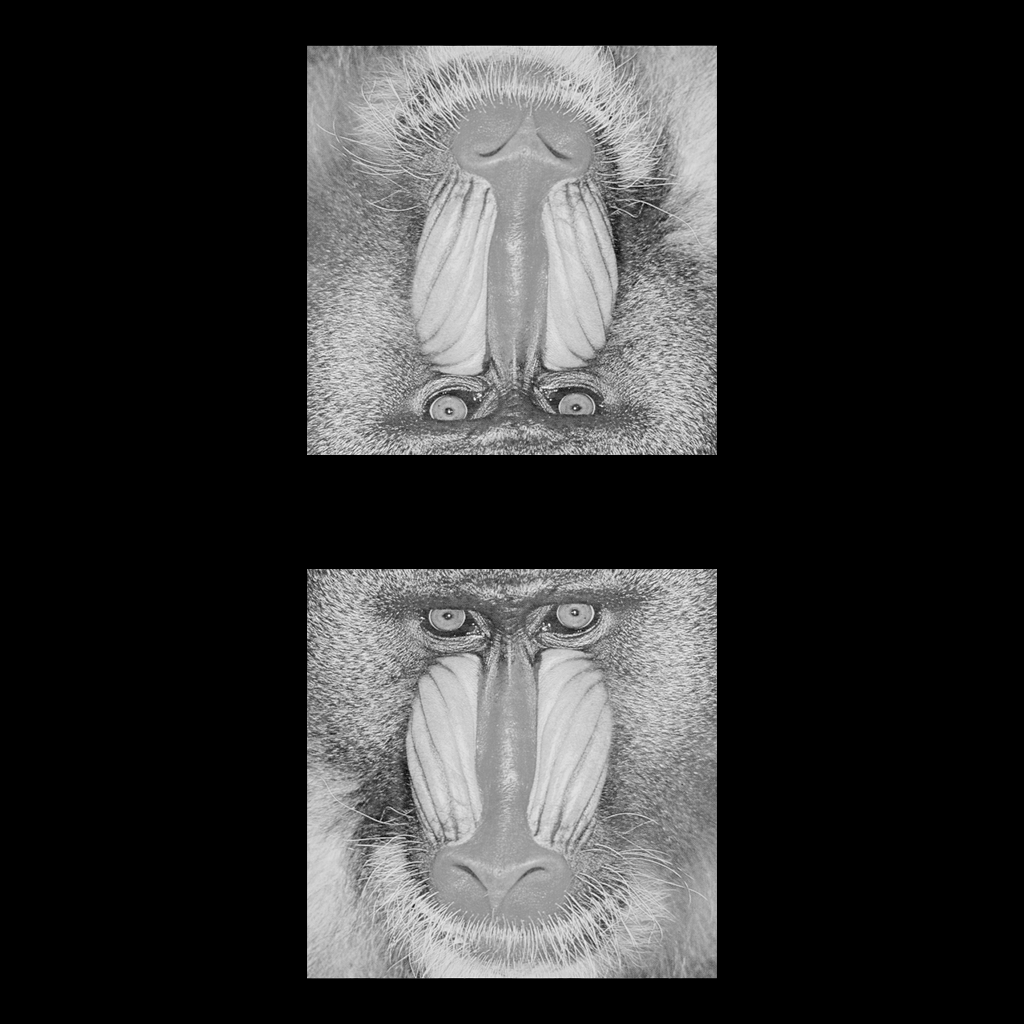
\includegraphics[width=\textwidth]{mandrill_2.png}
    \caption{Target image for the binary-phase SLM}
    \label{fig:mandrill_2}
  \end{subfigure}
  \hfill
  \begin{subfigure}[t]{0.3\textwidth}
    \centering
    
\includegraphics[width=\textwidth]{Naive_binary_Holo.png}
    \caption{Binary-phase Hologram}
    \label{fig:Naive_binary_Holo}
  \end{subfigure}
  \hfill
  \begin{subfigure}[t]{0.3\textwidth}
    \centering
    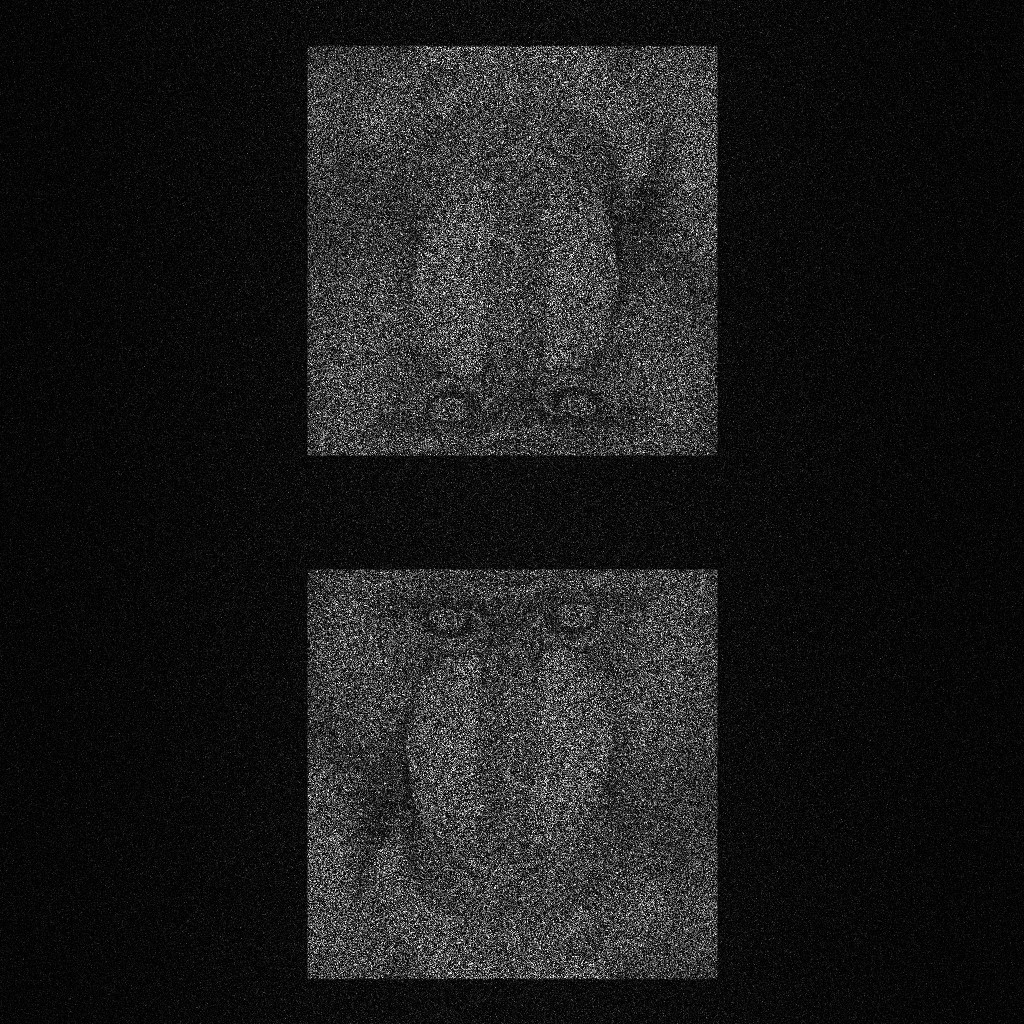
\includegraphics[width=\textwidth]{Naive_binary_Recon.jpg}
    \caption{Reconstruction}
    \label{fig:Naive_binary_Recon}
  \end{subfigure}
  \caption{Output of the improved Naive method with binary-phase quantisation}
  \label{fig:Output of the improved Naive method with binary-phase quantisation}
\end{figure}

The binary phase hologram in \cref{fig:Naive_binary_Holo} is generated by adding an additional binary quantisation step ($\mathcal{Q}$) on the phase hologram computed using \cref{alg:Naive algorithm with random phase}, which is simply rounding all phases to 0 rad and $\pi$ rad. The reconstruction of the binary-phase hologram is shown in \cref{fig:Naive_binary_Recon}, which is of poor quality with NMSE being \num{4.5452e-07} and SSIM being 0.0603. The only advantage of this method is its speed, as it only requires one inverse Fourier Transform calculation. To improve the reconstruction quality, better algorithms are needed. The following sections explores predecessors' efforts in quality improvement.

\newpage
\subsection{Direct Binary Search (DBS) Algorithm}\label{sec:Direct Binary Search (DBS) Algorithm}
Direct Binary Search (DBS) algorithm \cite{Seldowitz1987} is an algorithm that generates the hologram by randomly flipping each pixel in the SLM between binary states (0 and $\pi$), one by one for many times in order to minimise the difference between its reconstruction intensity $R$ and the target image $T$. The detailed algorithm is described in \cref{alg:DBS algorithm} below:
\begin{algorithm}[H]
  \caption{Direct Binary Search (DBS) algorithm}\label{alg:DBS algorithm}
  \textbf{Input:} Target image $T$, Propagation function $\mathcal{P}$, Loss function $\mathcal{L}$ (e.g. mean-squared error), Number of iterations $N$ \\
  \textbf{Output:} Phase hologram $H$ and its reconstruction intensity $R$
  \begin{algorithmic}
    \State{// Start with a random hologram with a size matching $T$}
    \State $H \gets$ Rand(Size($T$))
    \State $R \gets \vert \mathcal{P}[e^{jH}] \vert ^2$
    \State $L \gets \mathcal{L} [R, T]$

    \For {$n$ = $1$ to $N$}
    \State{// Flip a random pixel in the hologram}
    \State $H_n \gets$ FlipRandomPixel($H$)\\
    \State{// Calculate the loss function for the new hologram}
    \State $R_n \gets \vert \mathcal{P}[e^{jH_n}] \vert ^2$
    \State $L_n \gets \mathcal{L} [R_n, T]$\\
    \State{// Compare the new loss with the old one}
    \If {$L_n < L$}
    \State{// Accept the new hologram if loss is lower}
    \State $H \gets H_n$
    \State $R \gets R_n$
    \State $L \gets L_n$
    \EndIf
    \EndFor
  \end{algorithmic}
\end{algorithm}

Although the DBS algorithm is specifically suited for generating binary phase holograms, it can also be adapted for generating multi-level phase holograms, by representing each level as binary numbers, at the cost of more computation.

\begin{figure}[H]
  \centering
  \begin{subfigure}[t]{0.3\textwidth}
    \centering
    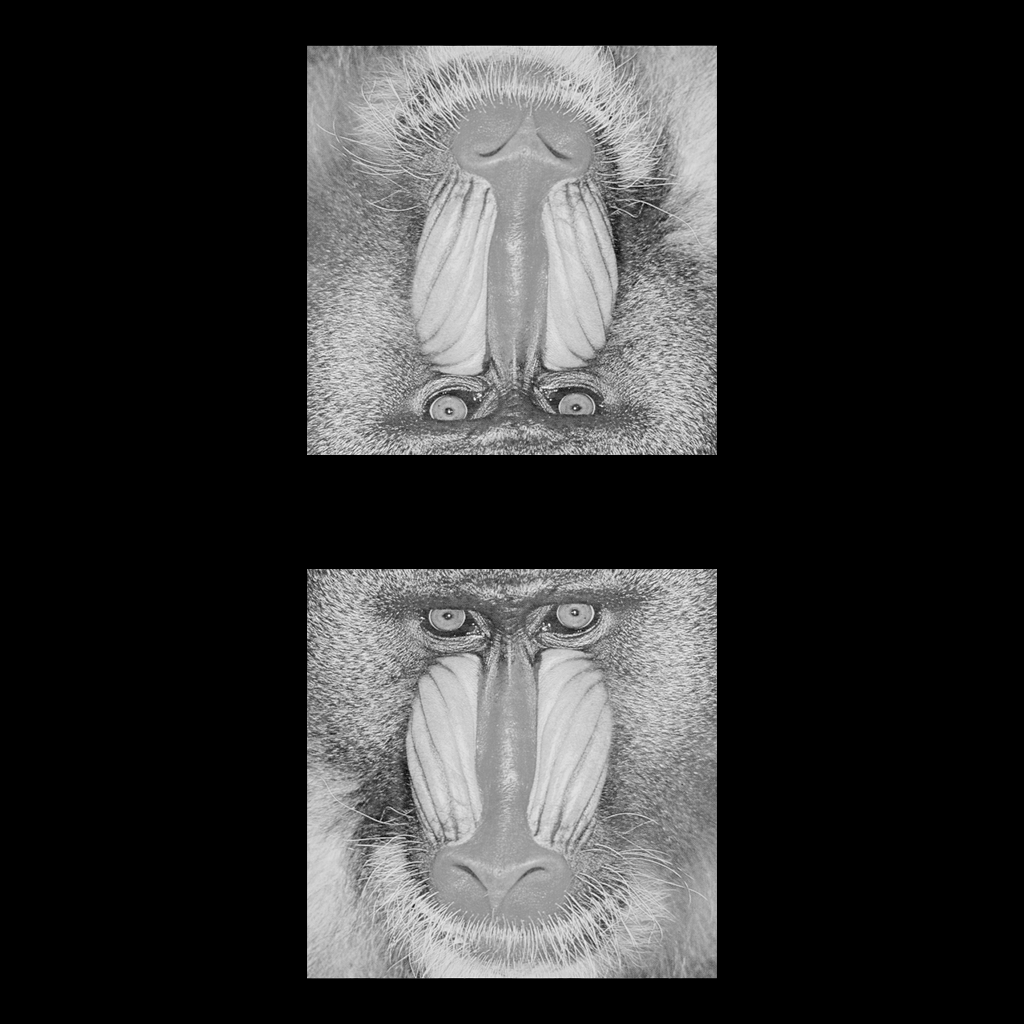
\includegraphics[width=\textwidth]{mandrill_2.png}
    \caption{Target image ($1024 px\times 1024 px$)}
    \label{fig:mandrill_2_DBS}
  \end{subfigure}
  \hfill
  \begin{subfigure}[t]{0.3\textwidth}
    \centering
    
\includegraphics[width=\textwidth]{DBS_mandrill_2_Holo.png}
    \caption{Binary-phase Hologram}
    \label{fig:DBS_mandrill_2_Holo}
  \end{subfigure}
  \hfill
  \begin{subfigure}[t]{0.3\textwidth}
    \centering
    
\includegraphics[width=\textwidth]{DBS_mandrill_2_recon_intensity.jpg}
    \caption{Reconstruction}
    \label{fig:DBS_mandrill_2_recon_intensity}
  \end{subfigure}
  \\
  \begin{subfigure}[t]{0.7\textwidth}
    \centering
    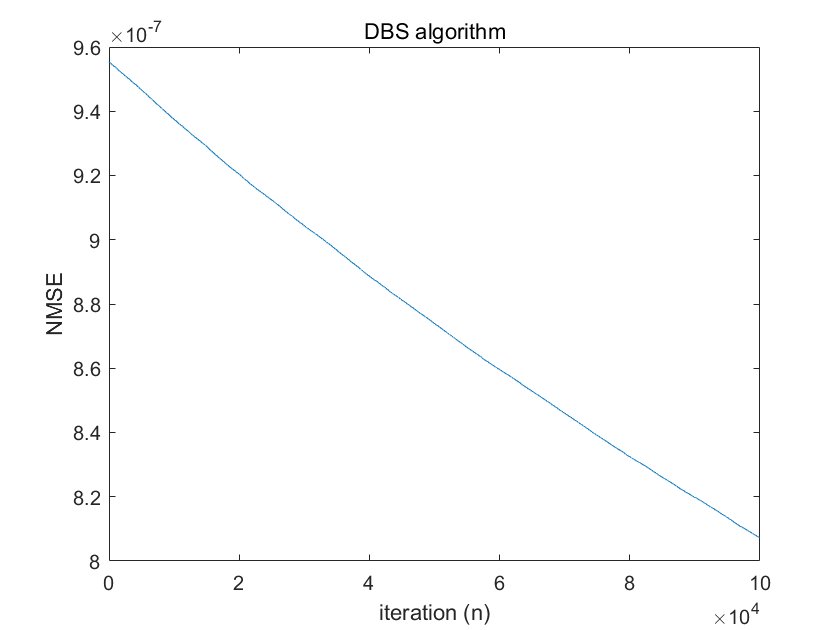
\includegraphics[width=\textwidth]{DBS_mandrill_2_convergence.png}
    \caption{NMSE v.s. iteration plot}
    \label{fig:DBS_mandrill_2_convergence}
  \end{subfigure}
  \caption{DBS algorithm running on the rotationally symmetrical mandrill target}
  \label{fig:DBS algorithm running on the rotationally symmetrical mandrill target}
\end{figure}

DBS algorithm can sometimes find very accurate hologram if the run is lucky; however, it is extremely slow, because it takes numerous iterations (as shown in \cref{fig:DBS_mandrill_2_convergence}, even $10^5$ iterations has not reached a good convergence) and each iteration requires a Fourier Transform which is computationally expensive, the example run on the target image of resolution $1024 px\times 1024 px$ in \cref{fig:mandrill_2_DBS} took more than one hour to run the $10^5$ iterations, which is still nowhere near convergence. The binary-phase hologram produced is shown in \cref{fig:DBS_mandrill_2_Holo} and its corresponding reconstruction in \cref{fig:DBS_mandrill_2_recon_intensity} is of very poor quality.

\begin{figure}[H]
  \centering
  \begin{subfigure}[t]{0.3\textwidth}
    \centering
    
\includegraphics[width=\textwidth]{test_128.png}
    \caption{Target image ($128 px\times 128 px$)}
    \label{fig:test_128}
  \end{subfigure}
  \hfill
  \begin{subfigure}[t]{0.3\textwidth}
    \centering
    
\includegraphics[width=\textwidth]{DBS_test_128_Holo.png}
    \caption{Binary-phase Hologram}
    \label{fig:DBS_test_128_Holo}
  \end{subfigure}
  \hfill
  \begin{subfigure}[t]{0.3\textwidth}
    \centering
    
\includegraphics[width=\textwidth]{DBS_test_128_recon_intensity.png}
    \caption{Reconstruction}
    \label{fig:DBS_test_128_recon_intensity}
  \end{subfigure}
  \\
  \begin{subfigure}[t]{0.7\textwidth}
    \centering
    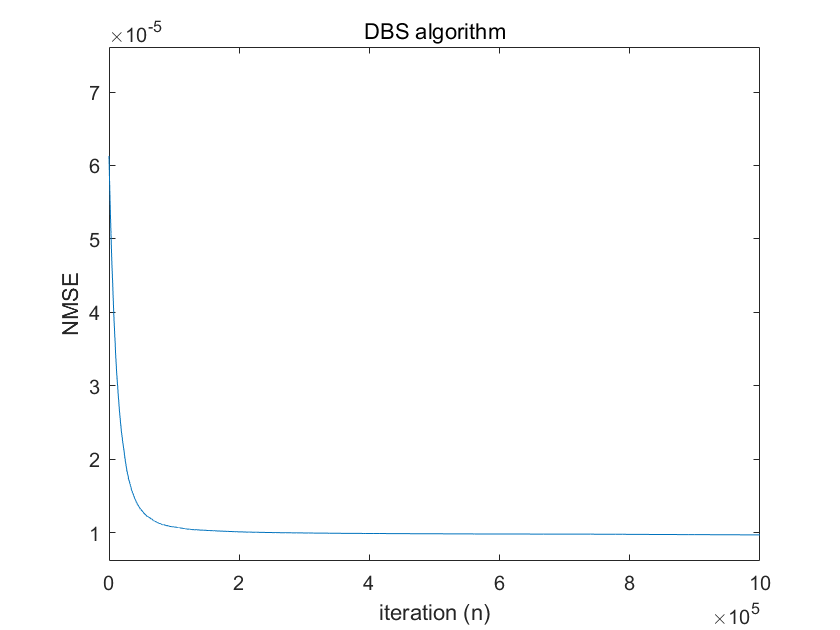
\includegraphics[width=\textwidth]{DBS_test_128_convergence.png}
    \caption{NMSE v.s. iteration plot}
    \label{fig:DBS_test_128_convergence}
  \end{subfigure}
  \caption{DBS algorithm running on the low resolution target}
  \label{fig:DBS algorithm running on the low resolution target}
\end{figure}

As the DBS algorithm only flips one pixel per iteration, it naturally takes significantly longer to generate holograms with higher resolution. To test the programme on a smaller image for much quicker convergence, another target image has been designed as shown in \cref{fig:test_128}, which is also rotationally symmetrical as it is used for the binary-phase hologram generation. After $10^6$ iterations, which took 10 minutes, the hologram generated is shown in \cref{fig:DBS_test_128_Holo} and its resulting reconstruction is shown in \cref{fig:DBS_test_128_recon_intensity}, which has an NMSE of \num{9.6881e-06} and an SSIM of 0.2871. The NMSE v.s. iteration plot in \cref{fig:DBS_test_128_convergence} shows that it reaches a good convergence at around \num{2e5} iterations, corresponding to around 2 minutes. And the curve of NMSE is monotonically decreasing with iteration number, as only holograms with better results are accepted during the iterations.

In summary, the DBS algorithm is a slow but working algorithm for binary phase hologram generation. The programme running time scales up significantly when the target image's resolution gets higher. And also, as it only cares about local optimality at each iteration, it is a greedy algorithm that only follow the steepest descent route, which could easily get trapped in a local minimum where flipping any bit is not getting better reconstruction. Another consequence of the random nature is that the generated hologram will be different at each run, so the quality of the resulting reconstruction ($R$) will depend on how `lucky' each run is. The Simulated Annealing (SA) algorithm \cite{Kirkpatrick1983} in the next session aims to resolve this issue.


\subsection{Simulated Annealing (SA) Algorithm}\label{sec:Simulated Annealing (SA) Algorithm}
Simulated Annealing (SA) algorithm \cite{Kirkpatrick1983} is a variant of the DBS algorithm. It adopts a probabilistic approach to avoid the steepest gradient descent. Its name derives from the fact that it approximates the recrystallisation process during metal annealing and is particularly well-suited to avoiding the trap of local minima \cite{Yang2009}. To implement this idea, we then need a function ($\mathcal{Z}$) to calculate the probability of the hologram ($H$), and a threshold $p_t$ to decide whether the probability is high enough for the according hologram to be accepted. In this thesis, the probability is selected to be a random function and the threshold is chosen to be 0.9. The pseudocode for this algorithm is listed in \cref{alg:Simulated Annealing (SA) algorithm}.
\begin{algorithm}[H]
  \caption{Simulated Annealing (SA) algorithm}\label{alg:Simulated Annealing (SA) algorithm}
  \textbf{Input:} Target image $T$, Propagation function $\mathcal{P}$, Loss function $\mathcal{L}$, Number of iterations $N$, Probability function $\mathcal{Z}$, Probability threshold $p_t$ \\
  \textbf{Output:} Phase hologram $H$ and its reconstruction intensity $R$
  \begin{algorithmic}
    \State{// Start with a random hologram with a size matching $T$}
    \State $H \gets$ Rand(Size($T$))
    \State $R \gets \vert \mathcal{P}[e^{jH}] \vert ^2$
    \State $L \gets \mathcal{L} [R, T]$

    \For {$n$ = $1$ to $N$}
    \State{// Flip a random pixel in the hologram}
    \State $H_n \gets$ FlipRandomPixel($H$)\\
    \State{// Calculate the loss function for the new hologram}
    \State $R_n \gets \vert \mathcal{P}[e^{jH_n}] \vert ^2$
    \State $L_n \gets \mathcal{L} [R_n, T]$\\
    \State{// Compare the new loss with the old one}
    \If {$L_n < L$}
    \State{// Accept the new hologram if loss is lower}
    \State $H \gets H_n$
    \State $R \gets R_n$
    \State $L \gets L_n$
    \Else
    \State{// Calculate the probability of the hologram}
    \State $p_n \gets \mathcal{Z}[H_n]$
    \If {$p_n > p_t$}
    \State{// Accept the new hologram if the probability exceeds the threshold}
    \State $H \gets H_n$
    \State $R \gets R_n$
    \State $L \gets L_n$
    \EndIf
    \EndIf
    \EndFor
  \end{algorithmic}
\end{algorithm}

\begin{figure}[H]
  \centering
  \begin{subfigure}[t]{0.3\textwidth}
    \centering
    
\includegraphics[width=\textwidth]{test_128.png}
    \caption{Target image ($128 px\times 128 px$)}
    \label{fig:test_128_SA}
  \end{subfigure}
  \hfill
  \begin{subfigure}[t]{0.3\textwidth}
    \centering
    
\includegraphics[width=\textwidth]{SA_test_128_Holo.png}
    \caption{Binary-phase Hologram}
    \label{fig:SA_test_128_Holo}
  \end{subfigure}
  \hfill
  \begin{subfigure}[t]{0.3\textwidth}
    \centering
    
\includegraphics[width=\textwidth]{SA_test_128_recon_intensity.png}
    \caption{Reconstruction}
    \label{fig:SA_test_128_recon_intensity}
  \end{subfigure}
  \\
  \begin{subfigure}[t]{0.7\textwidth}
    \centering
    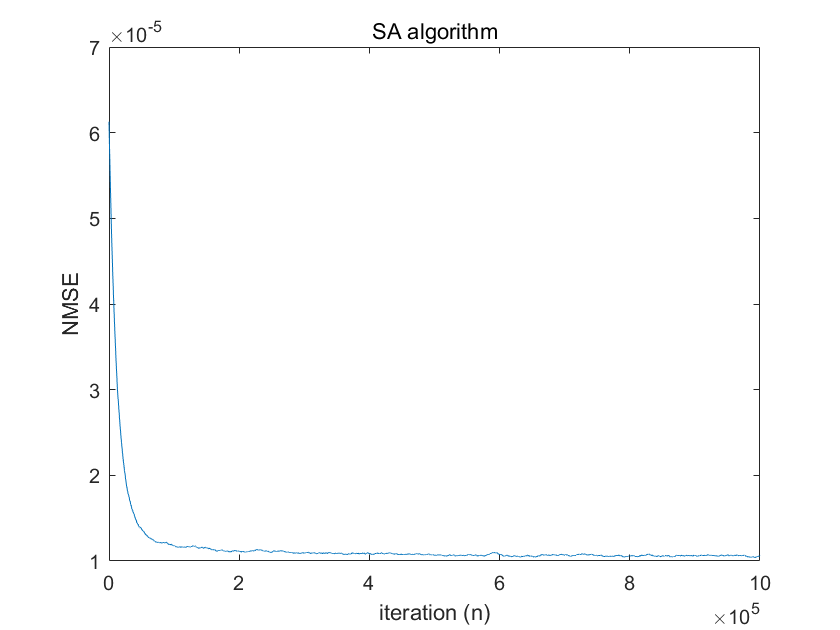
\includegraphics[width=\textwidth]{SA_test_128_convergence.png}
    \caption{NMSE v.s. iteration plot}
    \label{fig:SA_test_128_convergence}
  \end{subfigure}
  \caption{SA algorithm running on the low resolution target}
  \label{fig:SA algorithm running on the low resolution target}
\end{figure}

An implementation of SA algorithm with $p_t = 0.9$ was carried out on the low resolution target in \cref{fig:test_128_SA}, and the resulting binary-phase hologram and its reconstruction are shown in shown in \cref{fig:SA_test_128_Holo} and \cref{fig:SA_test_128_recon_intensity} respectively. From the NMSE v.s. iteration plot in \cref{fig:SA_test_128_convergence}, it can be seen that, instead of the monotonic decrease observed in \cref{fig:DBS_test_128_convergence} for DBS algorithm, the SA algorithm has occasional rises in NMSE, which happens when the probability $p_n$ exceeds the threshold $p_t$. The final NMSE was recorded to be \num{1.0542e-05} and the final SSIM was 0.2750, which are both slightly worse than the DBS algorithm in this case. Due to the probabilistic nature of the SA algorithm, although it can avoid being trapped in local optimal points, the `jump backs' can also cause delays in convergence.

\begin{figure}[H]
  \centering
  \begin{subfigure}[t]{0.3\textwidth}
    \centering
    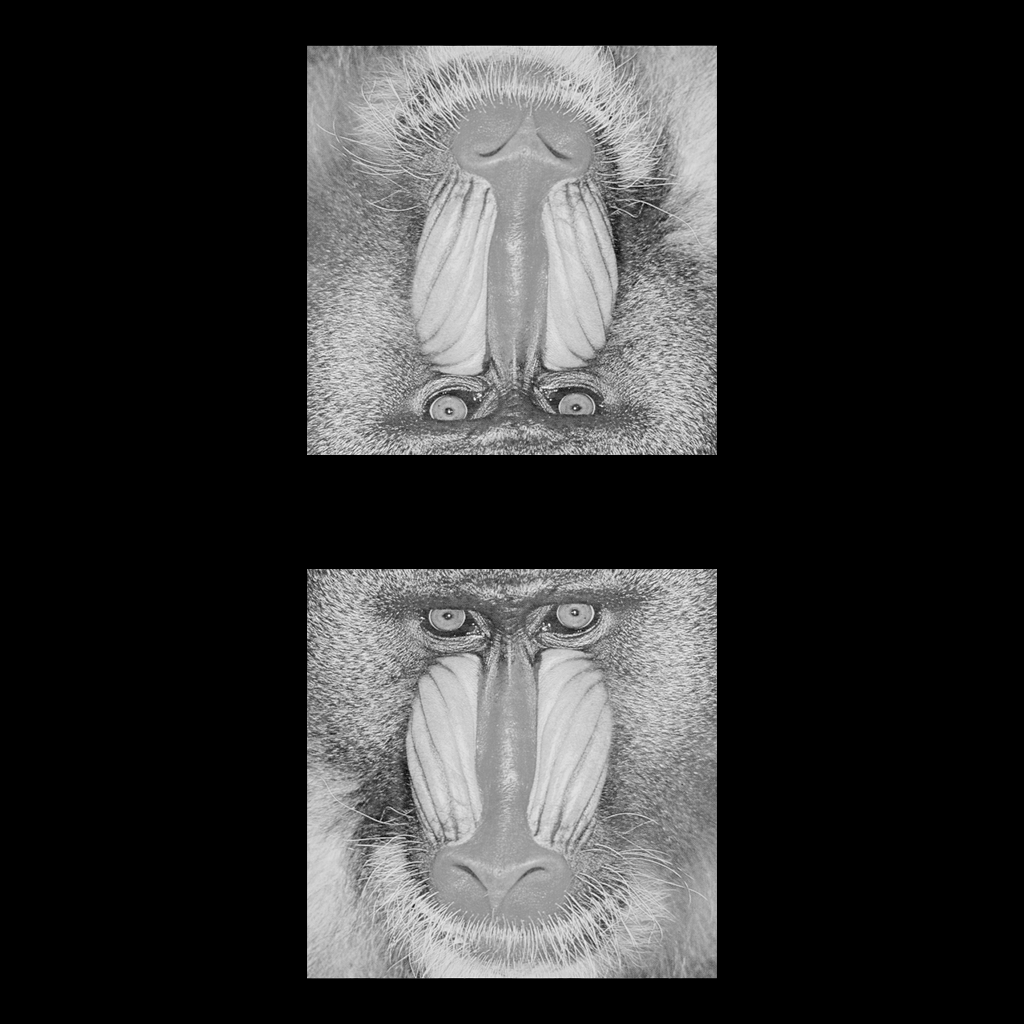
\includegraphics[width=\textwidth]{mandrill_2.png}
    \caption{Target image ($1024 px\times 1024 px$)}
    \label{fig:mandrill_2_SA}
  \end{subfigure}
  \hfill
  \begin{subfigure}[t]{0.3\textwidth}
    \centering
    
\includegraphics[width=\textwidth]{SA_mandrill_2_Holo.png}
    \caption{Binary-phase Hologram}
    \label{fig:SA_mandrill_2_Holo}
  \end{subfigure}
  \hfill
  \begin{subfigure}[t]{0.3\textwidth}
    \centering
    
\includegraphics[width=\textwidth]{SA_mandrill_2_recon_intensity.jpg}
    \caption{Reconstruction}
    \label{fig:SA_mandrill_2_recon_intensity}
  \end{subfigure}
  \\
  \begin{subfigure}[t]{0.7\textwidth}
    \centering
    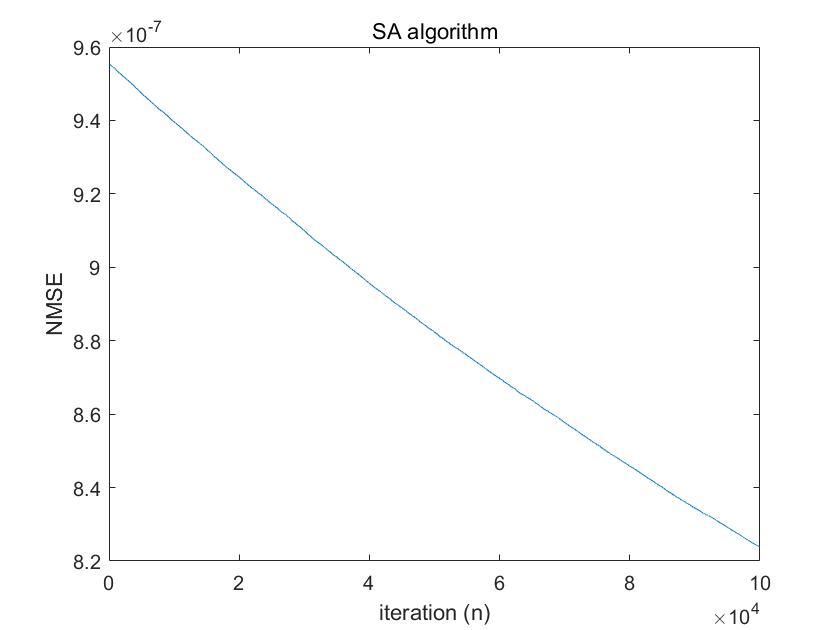
\includegraphics[width=\textwidth]{SA_mandrill_convergence.png}
    \caption{NMSE v.s. iteration plot}
    \label{fig:SA_mandrill_2_convergence}
  \end{subfigure}
  \caption{SA algorithm running on the rotationally symmetrical mandrill target}
  \label{fig:SA algorithm running on the rotationally symmetrical mandrill target}
\end{figure}

Then the SA algorithm was run for the mandrill target in \cref{fig:mandrill_2_SA}. The convergence plot in \cref{fig:SA_mandrill_2_convergence} shows that it did not converge within $10^5$ iterations, which took around one hour. The binary phase hologram generated is shown in \cref{fig:SA_mandrill_2_Holo} and its corresponding reconstruction intensity is shown in \cref{fig:SA_mandrill_2_recon_intensity}, which is of very poor quality. Both the DBS and the SA algorithms rely on flipping only a single pixel per iteration, which is very inefficient. A better algorithm should change the value of multiple pixels at every iteration for better efficiency.


\subsection{Gerchberg-Saxton (GS) Algorithm}\label{sec:Gerchberg-Saxton (GS) Algorithm}
The Gerchberg-Saxton (GS) algorithm \cite{Gerchberg1972} is a revolutionary algorithm and is much better and more robust than the algorithms introduced in the previous sections. Although being more than 50 years old, the GS algorithm is still frequently used and has lots of variants \cite{Yang1994, WANG2017, Zhou2019}. It functions by iteratively determining the phase profile of the hologram required to reconstruct a target image, looping between the hologram and the reconstruction plane, and applying constraints to each plane accordingly during each iteration. GS algorithm is very easy to implement, its pseudocode is shown in \cref{alg:Gerchberg-Saxton (GS) Algorithm}.

\begin{algorithm}[H]
  \caption{Gerchberg-Saxton (GS) Algorithm}\label{alg:Gerchberg-Saxton (GS) Algorithm}
  \textbf{Input:} Target image $T$, Propagation function $\mathcal{P}$, Number of iterations $N$, Initial phase $\varPhi$ (e.g. random, zeros, or other patterns) \\
  \textbf{Output:} Phase hologram $H$ and its reconstruction intensity $R$
  \begin{algorithmic}
    \State{// Initiate $E$ with amplitude $\sqrt{T}$ and initial phase $\varPhi$}
    \State $E \gets \sqrt{T} \times e^{j\varPhi}$
    \For {$n$ = $1$ to $N$}
    \State{// Compute the hologram plane}
    \State $A \gets \mathcal{P}^{-1}[E]$
    \State{// Apply the phase-only constraint at the hologram plane}
    \State $A \gets e^{j\angle A}$\\
    \State{// Compute the propagation for the new hologram}
    \State $E \gets \mathcal{P}[A]$
    \State{// Apply the target field amplitude constraint at the reconstruction plane}
    \State $E \gets \sqrt{T} \times e^{j\angle E}$
    \EndFor
    \State $H \gets \angle A$
    \State $R \gets \vert \mathcal{P}[A] \vert ^2$
  \end{algorithmic}
\end{algorithm}

The GS algorithm described in \cref{alg:Gerchberg-Saxton (GS) Algorithm} was implemented in MATLAB and was first run on the mandrill target image in \cref{fig:mandrill.png} the output results are shown in \cref{fig:GS algorithm output}. It can be seen from \cref{fig:GS_recon_i_30} that, the reconstruction after 30 iterations of GS algorithm reached a very good result, having an NMSE of \num{2.6612e-08} and an SSIM of 0.7940, which are both much better than the single-iteration Naive method's result in \cref{fig:Naive_rand_recon}.

\begin{figure}[H]
  \centering
  \begin{subfigure}[t]{0.3\textwidth}
    \centering
    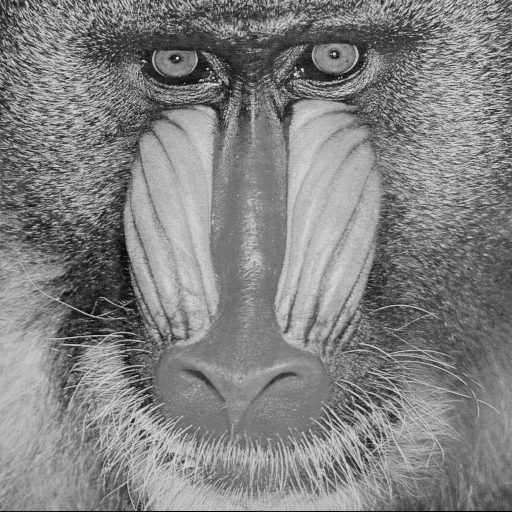
\includegraphics[width=\textwidth]{mandrill.png}
    \caption{Target image ($512 px\times 512 px$)}
  \end{subfigure}
  \hfill
  \begin{subfigure}[t]{0.3\textwidth}
    \centering
    
\includegraphics[width=\textwidth]{GS_holo_i_30.png}
    \caption{Hologram}
    \label{fig:GS_holo_i_30}
  \end{subfigure}
  \hfill
  \begin{subfigure}[t]{0.3\textwidth}
    \centering
    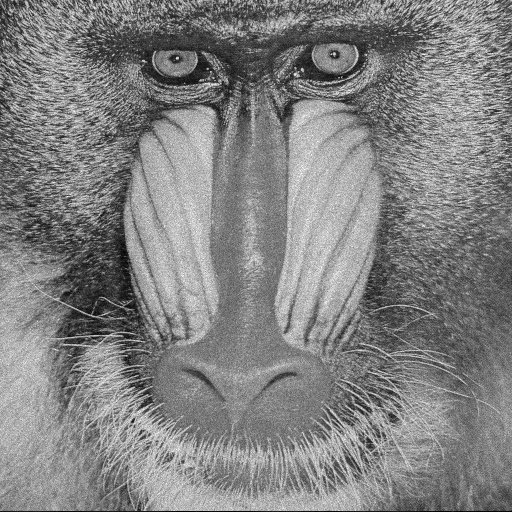
\includegraphics[width=\textwidth]{GS_recon_i_30.png}
    \caption{Reconstruction}
    \label{fig:GS_recon_i_30}
  \end{subfigure}
  \\
  \begin{subfigure}[t]{0.7\textwidth}
    \centering
    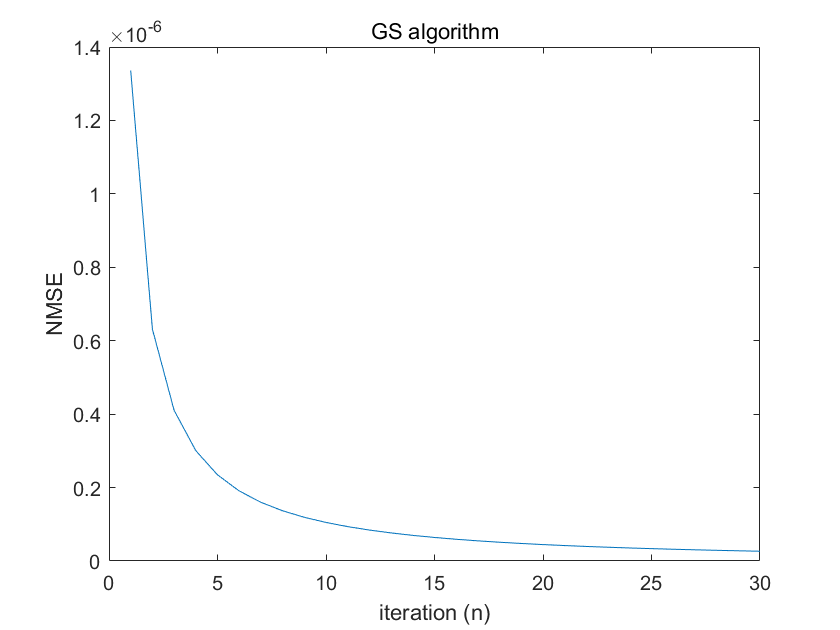
\includegraphics[width=\textwidth]{GS_NMSE_plot.png}
    \caption{NMSE v.s. iteration plot}
    \label{fig:GS_NMSE_plot}
  \end{subfigure}
  \caption{GS algorithm output on the mandrill target}
  \label{fig:GS algorithm output on the mandrill target}
\end{figure}


The NMSE v.s. iteration plot in \cref{fig:GS_NMSE_plot} shows that the GS algorithm converged quickly, providing very good result in tens of iterations, which is much fewer than the DBS and SA algorithms. Although the GS algorithm is more computationally expensive at each iteration, as it needs to compute both a forward and an backward propagation, leading to two Fourier transforms every iteration, the GS algorithm is still much faster and provides much better reconstruction quality than the DBS and SA algorithms.

\begin{figure}[H]
  \centering
  \begin{subfigure}[t]{0.3\textwidth}
    \centering
    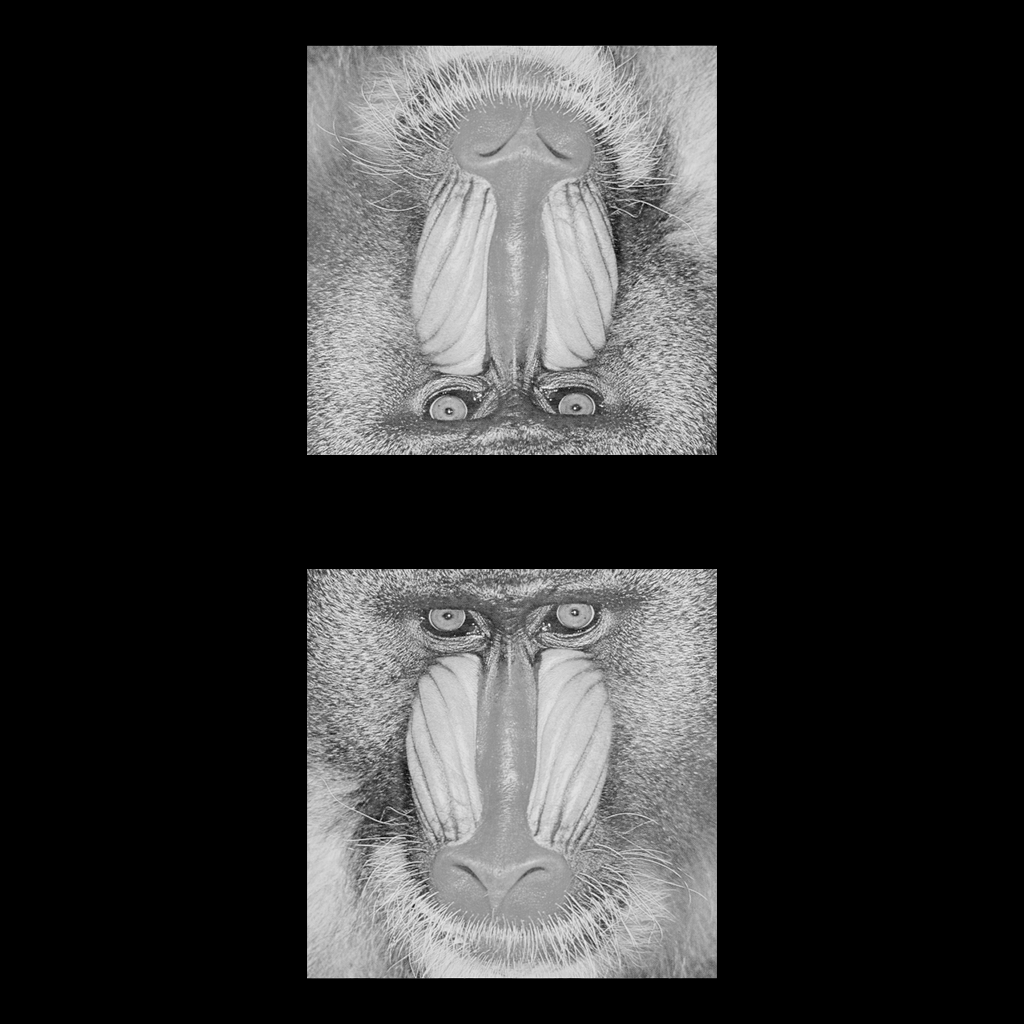
\includegraphics[width=\textwidth]{mandrill_2.png}
    \caption{Target image ($1024 px\times 1024 px$)}
    \label{fig:mandrill_2_GS}
  \end{subfigure}
  \hfill
  \begin{subfigure}[t]{0.3\textwidth}
    \centering
    
\includegraphics[width=\textwidth]{GS_Holo_mandrill_2.png}
    \caption{Binary-phase Hologram}
    \label{fig:GS_Holo_mandrill_2}
  \end{subfigure}
  \hfill
  \begin{subfigure}[t]{0.3\textwidth}
    \centering
    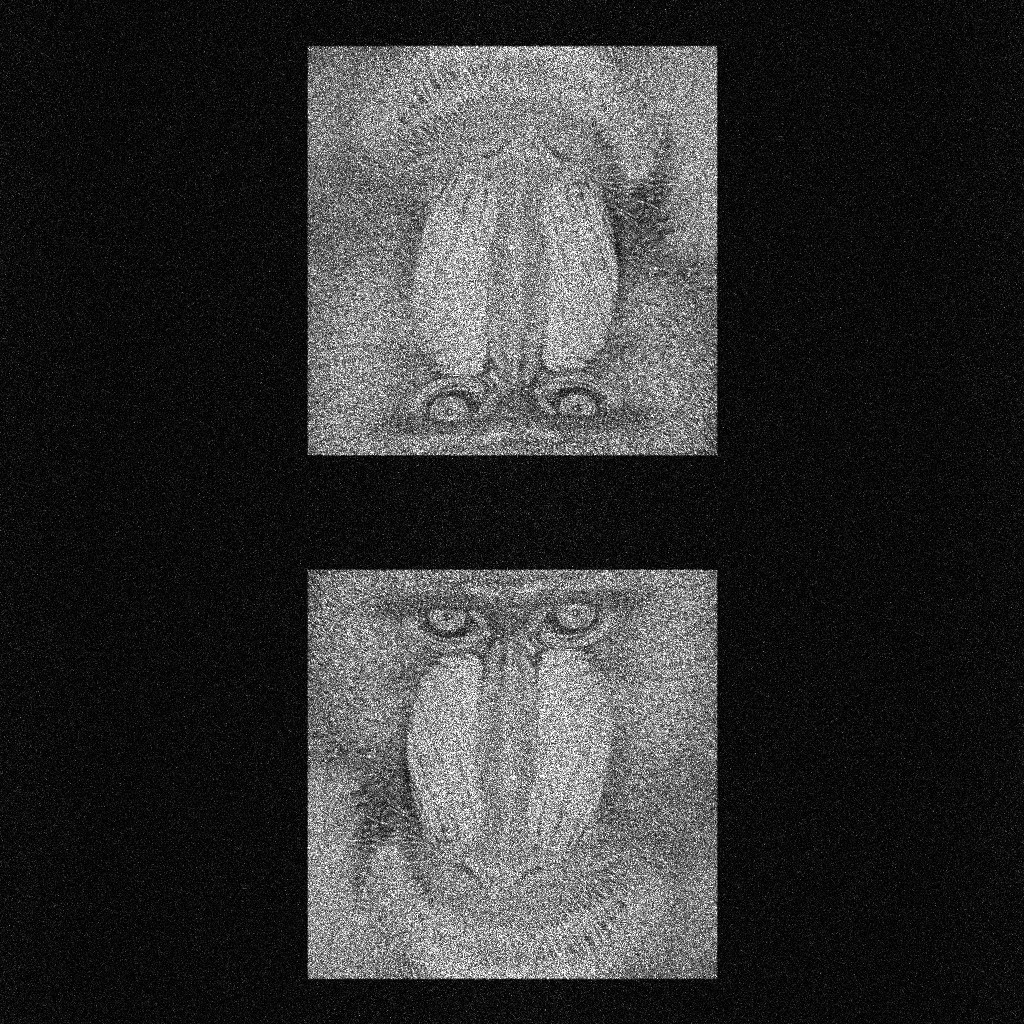
\includegraphics[width=\textwidth]{GS_Recon_mandrill_2.jpg}
    \caption{Reconstruction}
    \label{fig:GS_Recon_mandrill_2}
  \end{subfigure}
  \\
  \begin{subfigure}[t]{0.7\textwidth}
    \centering
    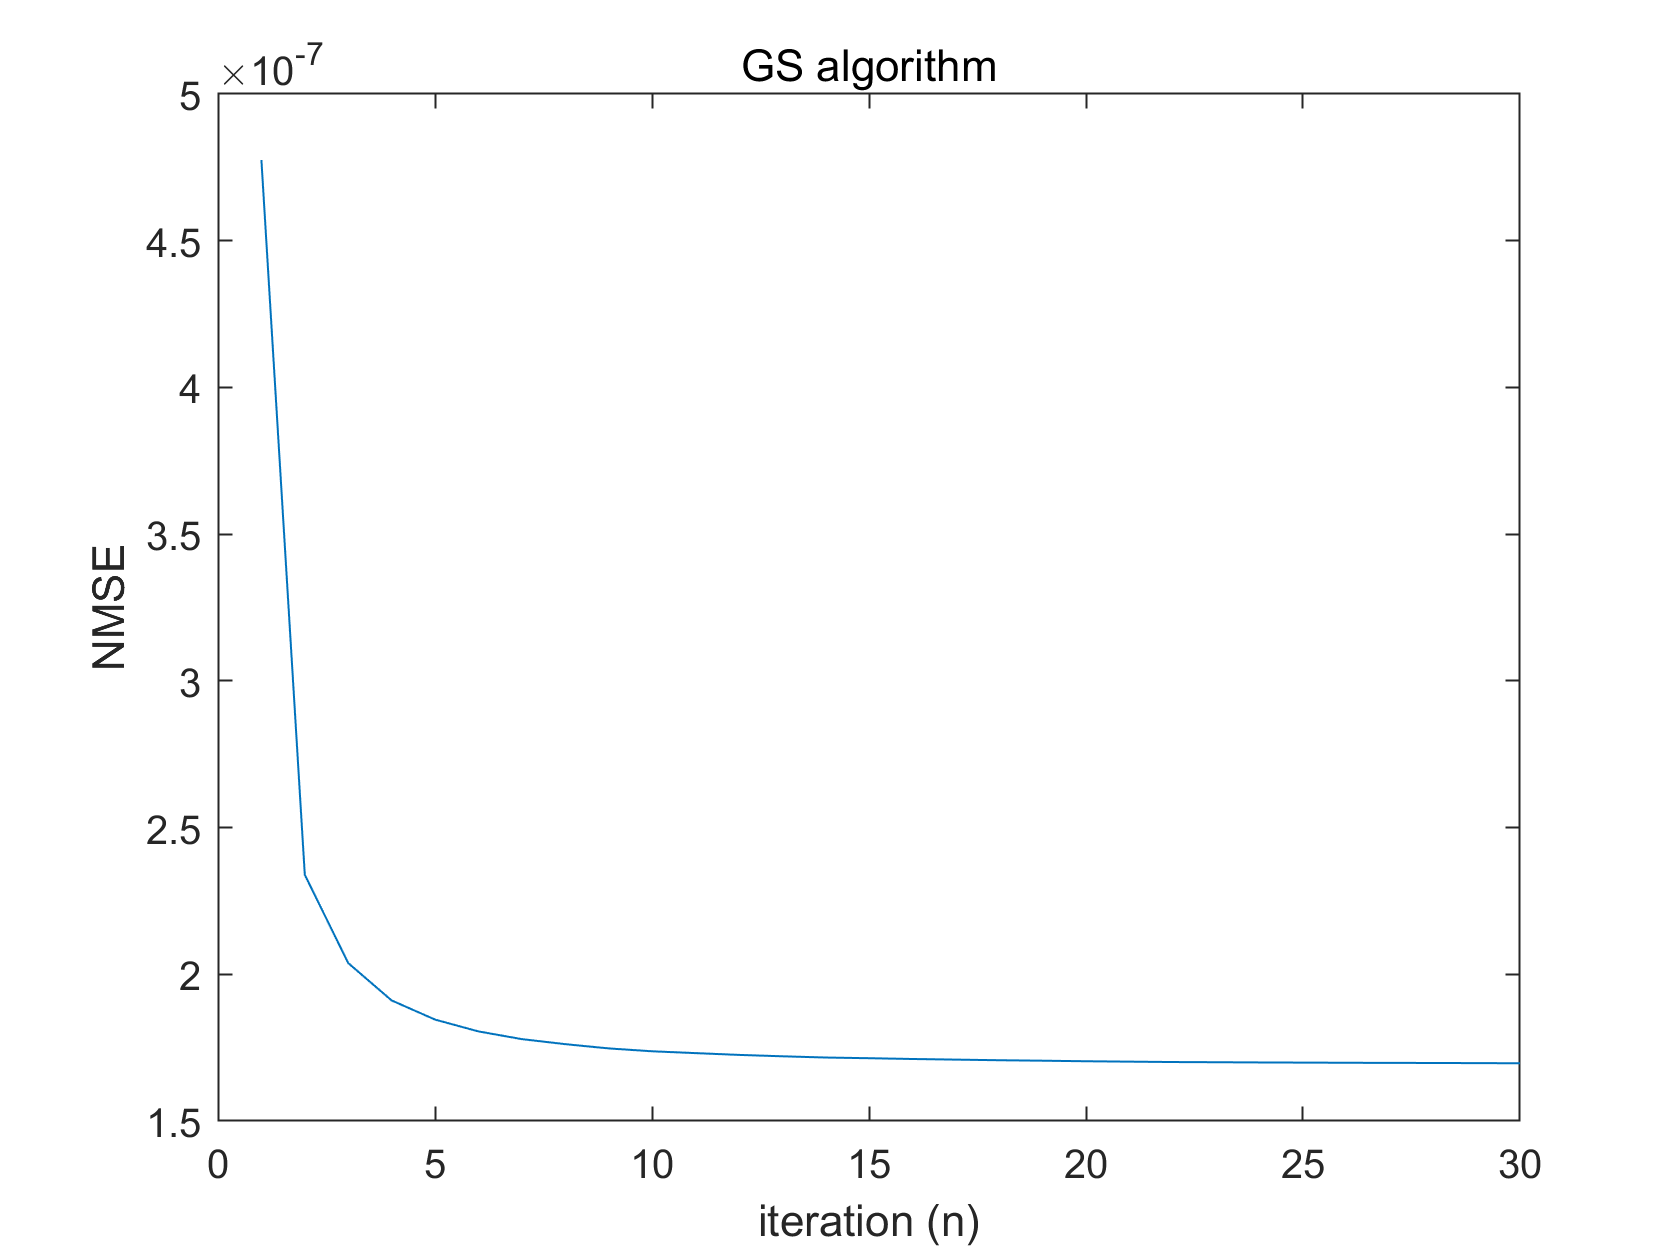
\includegraphics[width=\textwidth]{GS_mandrill_2_convergence.png}
    \caption{NMSE v.s. iteration plot}
    \label{fig:GS_mandrill_2_convergence}
  \end{subfigure}
  \caption{GS algorithm running on the rotationally symmetrical mandrill target}
  \label{fig:GS algorithm running on the rotationally symmetrical mandrill target}
\end{figure}

Then the GS algorithm was adapted to generate binary-phase holograms, for use on the binary-phase SLM in this thesis. The change was simply implemented by adding a quantisation function ($\mathcal{Q}$) when applying the phase-only constraint at the hologram plane (i.e. the line `$A \gets e^{j\angle A}$' in \cref{alg:Gerchberg-Saxton (GS) Algorithm} is changed to `$A \gets e^{j\mathcal{Q}[\angle A]}$'). The results are shown in \cref{fig:GS algorithm running on the rotationally symmetrical mandrill target}. \cref{fig:GS_mandrill_2_convergence} shows good convergence within 20 iterations. The resulting binary-phase hologram is shown in \cref{fig:GS_Holo_mandrill_2} and its corresponding reconstruction in \cref{fig:GS_Recon_mandrill_2} has an NMSE of 1.6968e-07 and an SSIM of 0.0619, which are both better than the Naive method's result in \cref{fig:Output of the improved Naive method with binary-phase quantisation}. In summary, the GS algorithm is quick and robust. On my laptop computer of model ASUS ROG Zephyrus M16, which has a CPU of model i7-11800H and a GPU of model RTX3060, the 30 iterations took 1.5 seconds to complete. It reached convergence in tens of iterations. However, as it is still iterative, generating holograms in real-time is still a challenge, and the reconstruction still suffers from noise.


\subsection{One-Step Phase Retrieval (OSPR) Algorithm}\label{sec:One Step Phase Retrieval (OSPR) Algorithm}
OSPR algorithm was first demonstrated by Buckley \cite{Buckley2006}. It is a solution to high-quality hologram reconstruction that relies on time multiplexing of holograms, exploiting the response time of eye in order to reduce noise in the replay field \cite{Cable2006}. The random noises are averaged by the eye, while the target image stays, so that the average noise can be reduced. The perceived noise is lessened by the temporal average detected by the eye, rather than computational optimisation of the hologram \cite{Cable2006}. The pseudocode for OSPR is shown in \cref{alg:One-Step Phase Retrieval (OSPR) algorithm} below.

\begin{algorithm}[H]
  \caption{One-Step Phase Retrieval (OSPR) algorithm}\label{alg:One-Step Phase Retrieval (OSPR) algorithm}
  \textbf{Input:} Target image $T$, Propagation function $\mathcal{P}$, Number of sub-frames $S$, Quantisation function $\mathcal{Q}$\\
  \textbf{Output:} List of phase holograms $H[1\ldots S]$
  \begin{algorithmic}
    \State // Compute a list of hologram sub-frames
    \For {$i$ = $1$ to $S$}
    \State $E \gets \sqrt{T} \times $ RandomPhase()
    \State $A \gets \mathcal{P}^{-1}[E]$
    \State $H[i] \gets \mathcal{Q}[\angle A]$
    \EndFor\\
    \State // Then display the sub-frames on the phase modulator sequentially
    \State $i\gets 1$
    \While {True}
    \State Display($H[i]$)
    \State $i\gets i + 1$
    \If {$i > S$}
    \State $i\gets 1$
    \EndIf
    \EndWhile
  \end{algorithmic}
\end{algorithm}

When generating the list of holograms, it repetitively computes the inverse propagation of the target amplitude (which is the square-root of the target intensity $T$) multiplied by different random phases, for a total of $S$ times to generate $S$ hologram sub-frames ($H[1\ldots S]$). The computation of each hologram sub-frame is the same as the Naive method in \cref{alg:Naive algorithm with random phase} discussed in \cref{sec:Naive algorithm}. Then the $S$ hologram sub-frames are displayed sequentially on a SLM having a refresh rate being so fast that the average reconstruction intensity is perceived by the human eyes. As currently available fast SLMs are binary-phase modulators, an example run on the rotationally symmetrical target previously used in \cref{fig:mandrill_2_DBS} was carried out for 24 sub-frames ($S=24$). The results are summarised in \cref{fig:ospr_mandrill_2}.

\begin{figure}[H]
	\centering
	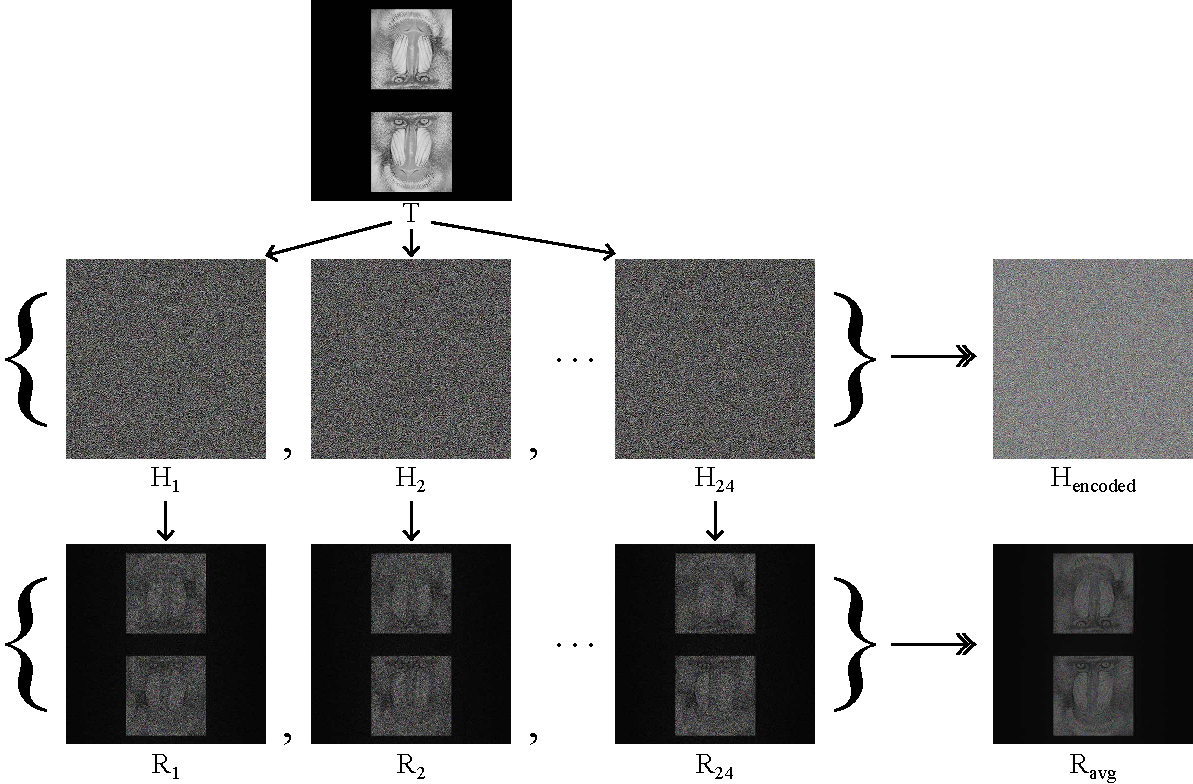
\includegraphics[width=1.0\textwidth]{ospr_mandrill_2.pdf}
	\caption{OSPR algorithm running on the rotationally symmetrical mandrill target}
	\label{fig:ospr_mandrill_2}
\end{figure}

In \cref{fig:ospr_mandrill_2}, a total of 24 binary-phase hologram sub-frames ($H_1, H_2, \ldots, H_{24}$) were generated for the target image $T$. For easier data transfer and to fit with the common display signal formats, the 24 binary-phase hologram sub-frames are encoded into a single file with 8 bit depth and RGB (red-green-blue) channels, so that each of the $(8\times 3 = )24$ bit-planes corresponds to a single binary-phase hologram sub-frame. For a quantitative analysis, the reconstruction intensities of the hologram sub-frames are computed in $R_1, R_2, \ldots, R_{24}$ respectively, whose average is $R_{avg}$ in \cref{fig:ospr_mandrill_2}. The average reconstruction intensity $R_{avg}$ has an NMSE of \num{9.8632e-08} and an SSIM of 0.1321, which are both significantly better than the GS algorithm (NMSE=\num{1.6968e-7}, SSIM=0.0619) and the Naive method (NMSE=\num{4.5452e-7}, SSIM=0.0603).

The major advantage of the OSPR algorithm is that it is superfast. It is non-iterative and requires only one Fourier Transform per frame, taking less than a second to generate a 24-frame hologram set. Its non-iterative nature also allows it to be parallelised to further improve computation speed, which is crucial for the Light Blue Optics who made the real-time holographic laser projector commercially available in 2010 \cite{Buckley2008}, although the product was later discontinued for financial reasons. The downside of this algorithm is that the sub-frames are independent from each other, and the final reconstruction output is still subject to some noise, as they are only more randomly distributed instead of being reduced. There is a variant of slight improvement on the OSPR algorithm, called Adaptive OSPR (AD-OSPR), to be introduced in \cref{sec:Adaptive One-Step Phase Retrieval (AD-OSPR) Algorithm}.



\subsection{Adaptive One-Step Phase Retrieval (AD-OSPR) Algorithm}\label{sec:Adaptive One-Step Phase Retrieval (AD-OSPR) Algorithm}

The AD-OSPR algorithm \cite{Kaczorowski2016} is a variant of the OSPR algorithm. It aims to improve the reconstruction quality without introducing a significant amount of additional computational cost. It functions in such a way that, when computing the second sub-frame onwards, it subtracts the average reconstruction from the target image to get the error, so that it can compensated in the next iteration. To help explain the process in detail, a pseudocode is written for the AD-OSPR algorithm, as shown in \cref{alg:Adaptive One-Step Phase Retrieval (AD-OSPR) algorithm}.

\begin{algorithm}[H]
  \caption{Adaptive One-Step Phase Retrieval (AD-OSPR) algorithm}\label{alg:Adaptive One-Step Phase Retrieval (AD-OSPR) algorithm}
  \textbf{Input:} Target image $T$, Propagation function $\mathcal{P}$, Number of sub-frames $S$, Quantisation function $\mathcal{Q}$\\
  \textbf{Output:} List of phase holograms $H[1\ldots S]$
  \begin{algorithmic}
    \State // Compute a list of hologram sub-frames
    \State $T[1] \gets T$
    \State $R_{avg}[0] \gets 0$
    \For {$i$ = $1$ to $S$}
    \State $E \gets \sqrt{T[s]} \times$ RandomPhase()
    \State $A \gets \mathcal{P}^{-1}[E]$
    \State $H[i] \gets \mathcal{Q}[\angle A]$\\

    \State // Compute average reconstruction
    \State $R \gets \vert \mathcal{P}[e^{jH[i]}] \vert ^2$
    \State $R_{avg}[i] \gets (R_{avg}[i-1] \times (i-1) + R)/i$\\

    \State // Update the target for the next iteration
    \State $T[i+1] \gets T + T - R_{avg}[i]$
    \EndFor\\

    \State // Then display the sub-frames on the phase modulator sequentially
    \State $i\gets 1$
    \While {True}
    \State Display($H[i]$)
    \State $i\gets i + 1$
    \If {$i > S$}
    \State $i\gets 1$
    \EndIf
    \EndWhile
  \end{algorithmic}
\end{algorithm}

In the pseudocode in \cref{alg:Adaptive One-Step Phase Retrieval (AD-OSPR) algorithm}, the target intensity for the first iteration ($T[1]$) is initialised as the input target image $T$, and the average reconstruction intensity for the holograms generated up to each iteration ($R_{avg}[i]$) is initialised as 0. Then the $\textbf{for}$ loop starts from the same routine as the OSPR algorithm, multiplying a random phase to the square root of target intensity, taking a inverse propagation, and applying the binary phase quantisation. Then, the average reconstruction is computed by propagating the quantised hologram of each iteration and take the weighted average between the current reconstruction intensity and the historical average reconstruction value. The average reconstruction is then used to update the target intensity for the next iteration, by subtracting the average from the target and adding the difference to the input target image. To provide a visual illustration, an example run of the AD-OSPR algorithm was carried out on the mandrill target as shown in \cref{fig:adospr_mandrill_2}.

\begin{figure}[H]
	\centering
	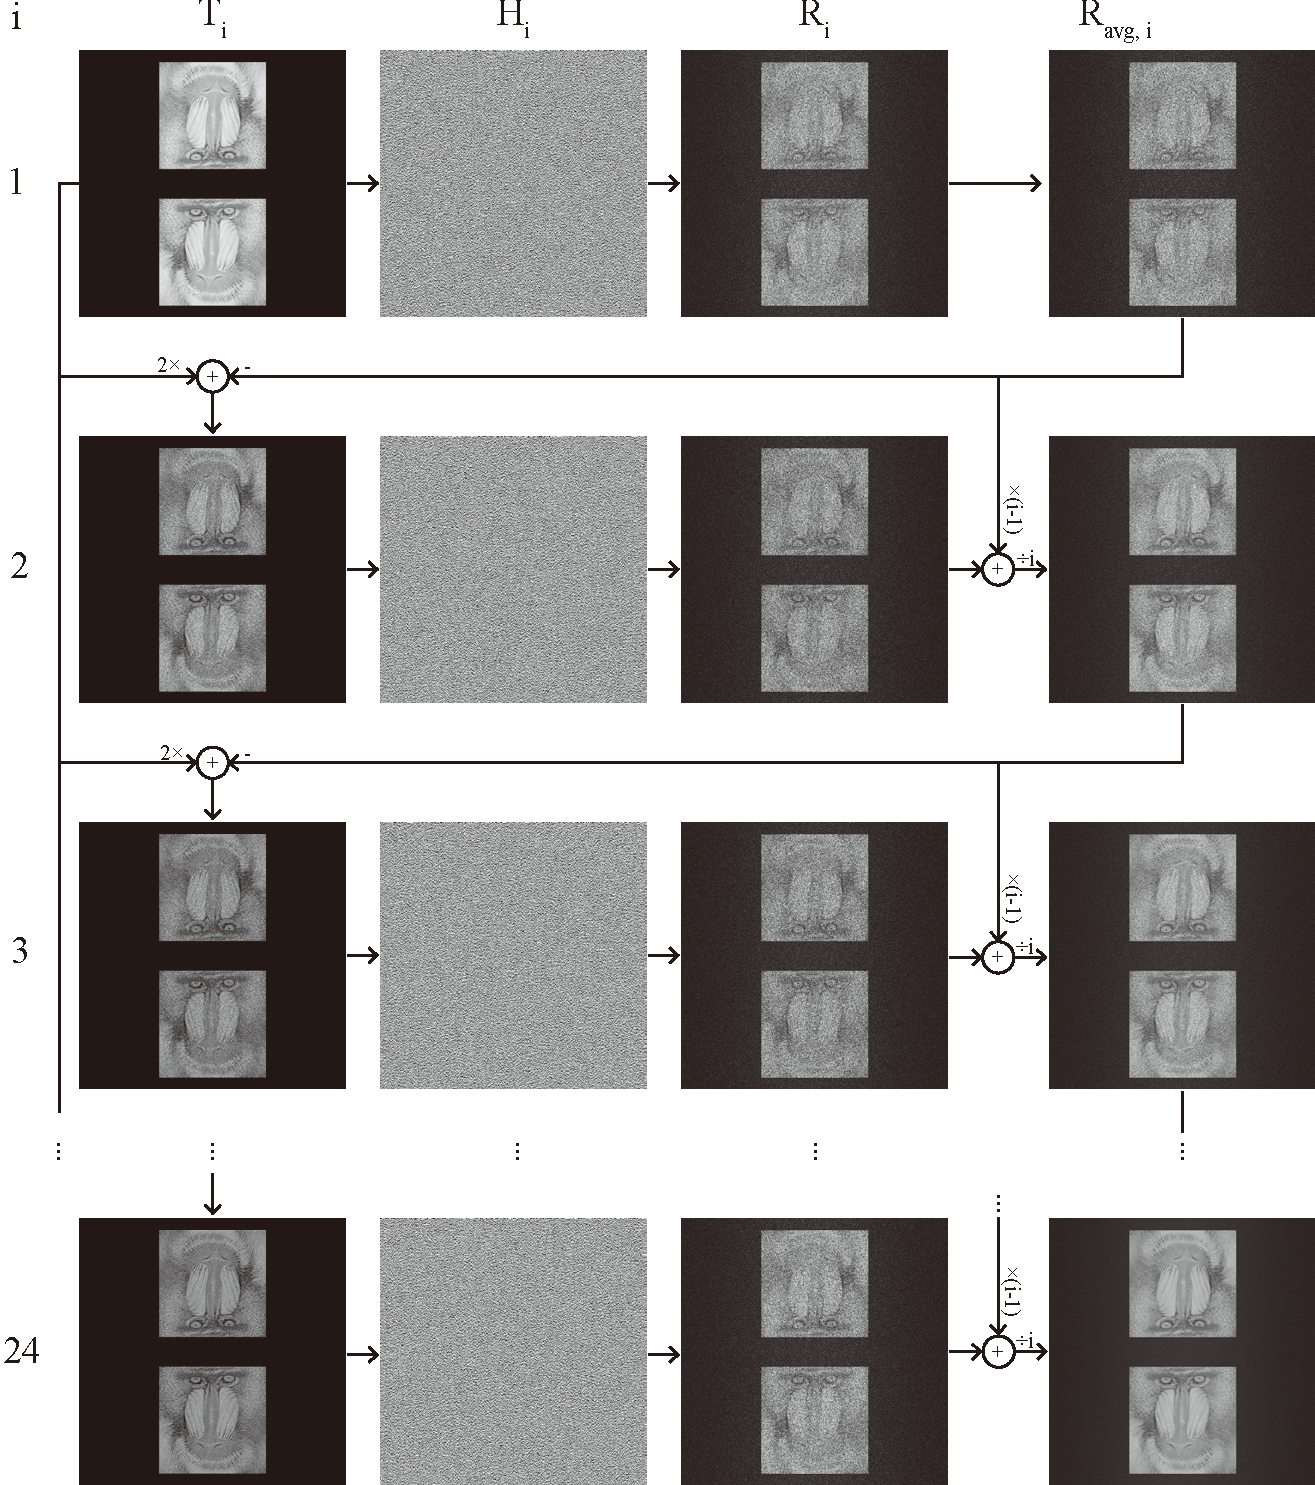
\includegraphics[width=1.0\textwidth]{adospr_mandrill_2.pdf}
	\caption{AD-OSPR algorithm running on the rotationally symmetrical mandrill target}
	\label{fig:adospr_mandrill_2}
\end{figure}

In \cref{fig:adospr_mandrill_2}, each row of images correspond to one iteration that is indexed in the `i' column, where only iterations 1, 2, 3, 24 are shown here, while iterations 4-23 are omitted to save space. At each iteration, the binary-phase hologram $H_i$ is computed from its target $T_i$, and the corresponding reconstruction is shown in $R_i$. For the first iteration, the target image of the same one as in \cref{fig:ospr_mandrill_2} is used, and the first average reconstruction $R_{avg, 1}$ is just the first reconstruction $R_1$. Then, from the second iteration, the target intensity $T_i$ is updated as the target image ($T$) plus the difference between the target image and the average reconstruction so far ($T-R_{avg, i}$). After computing new reconstructions $R_i$, the average reconstruction $R_{avg, i}$ is updated using the weighted average function $R_{avg}[i] \gets (R_{avg}[i-1] \times (i-1) + R)/i$. After 24 iterations, the 24 hologram sub-frames are computed and their average reconstruction ($R_{avg, 24}$) had an NMSE of \num{9.1161e-08} and a SSIM of 0.1992, which are both better than the OSPR algorithm in \cref{sec:One Step Phase Retrieval (OSPR) Algorithm} who achieved an NMSE of \num{9.8632e-08} and an SSIM of 0.1321.

The programme running time of the AD-OSPR algorithm is nearly the same as the OSPR algorithm, both being around 0.7 second. Therefore the AD-OSPR algorithm is quite an effective improvement on the original OSPR algorithm, achieving a 7.6\% reduction in NMSE and 50.8\% improvement in SSIM without adding much computation. The disadvantage is however, that it cannot be parallelised, unlike the OSPR algorithm. As it needs to have the average reconstruction intensity result from the previous iteration for use in the next iteration.


\newpage
\subsection{3D CGH}
\cref{sec:Naive algorithm} - \cref{sec:Adaptive One-Step Phase Retrieval (AD-OSPR) Algorithm} described several algorithms to generate a phase hologram for a single target image. However, the major benefit of holography is that it can produce true 3D light field, much more than just a single slice 2D image. Then the problem arises as how to generate a hologram for 3D targets to make full use of the major benefit of holography. The simplest method is to slice the 3D target into a set of 2D layers, like computed tomography (CT) scanning, and then generate a hologram so that its Fresnel propagation (in \cref{eq:fresnel-diffraction}) at each depth ($z$) matches the according layer. This subsection therefore reviews how the current methods in \cref{sec:Naive algorithm} - \cref{sec:Adaptive One-Step Phase Retrieval (AD-OSPR) Algorithm} can be adapted to multi-depth hologram generation.

\begin{figure}[H]
	\centering
	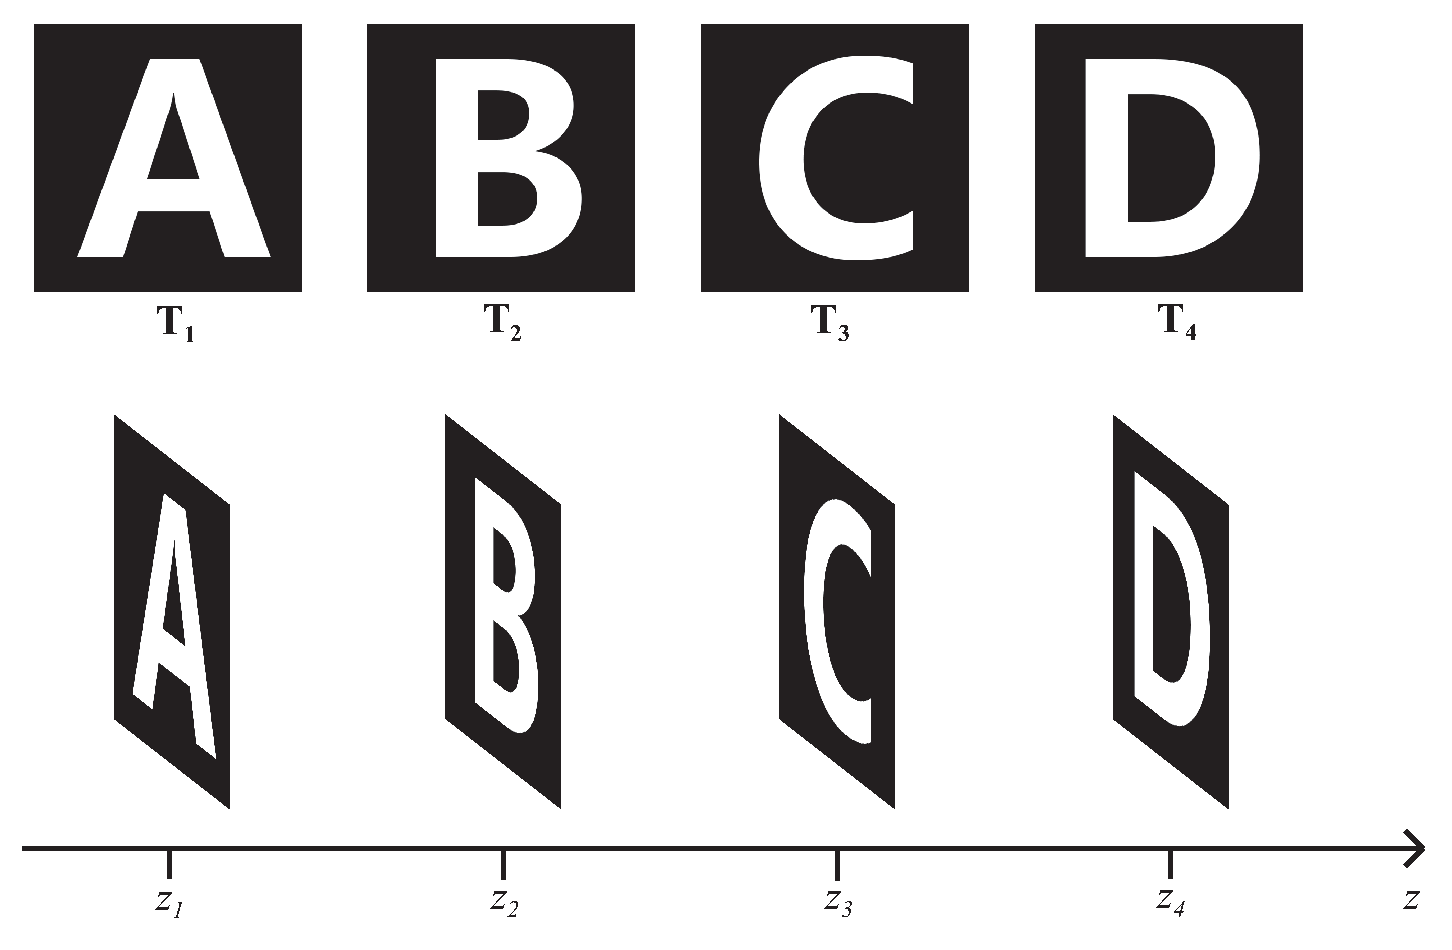
\includegraphics[width=1.0\textwidth]{ABCD/ABCD_target.eps}
	\caption{Multi-slice target consisted of 4 different characters at different distances}
	\label{fig:ABCD_target}
\end{figure}

For fair tests on algorithms, an example 3D target field consisted of 4 slices has been created using alphabets, as shown in \cref{fig:ABCD_target}. $T_1$ to $T_4$ have the same resolution of $512px \times 512px$, and the distances $z_1$ to $z_4$ are set to $1, 2, 3, 4 cm$ respectively.


\subsubsection{Naive phase addition}
To adapt the naive method in \cref{sec:Naive algorithm} to compute multi-depth hologram, firstly, a set of holograms are generated corresponding to each layer of the target field respectively, using the inverse of the Fresnel propagation function in \cref{eq:fresnel-diffraction}. Then, based on the principle of superposition, the set of holograms are added up to form the final hologram, whose phase is directly extracted to be the phase-only hologram while the amplitude component is discarded.

\begin{figure}[H]
	\centering
	\includegraphics[width=1.0\textwidth]{ABCD/Naive_ABCD.pdf}
	\caption{Naive phase addition method's result on the 4-slice target}
	\label{fig:Naive_ABCD}
\end{figure}

The simulation results shown in \cref{fig:Naive_ABCD} demonstrates the effectiveness of the naive phase addition method. The reconstructions at each depth are legible, despite the presence of some noise. However, after applying a binary-phase quantisation on the hologram, the reconstruction quality deteriorates significantly, as shown in \cref{fig:Naive_ABCD_binary}.

\begin{figure}[H]
	\centering
	\includegraphics[width=1.0\textwidth]{ABCD/Naive_ABCD_binary.pdf}
	\caption{Naive phase addition method's result on the 4-slice target after binary quantisation}
	\label{fig:Naive_ABCD_binary}
\end{figure}

To improve the reconstruction quality, the time-multiplexed OSPR algorithm (in \cref{sec:One Step Phase Retrieval (OSPR) Algorithm}) is adapted to produce multi-frame holograms for 3D targets.


\subsubsection{OSPR algorithm adaptation}
\begin{figure}[H]
	\centering
	\includegraphics[width=1.0\textwidth]{ABCD/OSPR_ABCD.pdf}
	\caption{OSPR algorithm's result on the 4-slice target}
	\label{fig:OSPR_ABCD}
\end{figure}

The OSPR algorithm in \cref{sec:One Step Phase Retrieval (OSPR) Algorithm} was adapted to generate multi-depth targets by doing the Naive phase addition method $S$ times, where $S$ is the total number of sub-frames. The results of the example run with $S=24$ is shown in \cref{fig:OSPR_ABCD}. The average reconstructions has much less noise than the single frame one in \cref{fig:Naive_ABCD_binary}. However, the contrast is rather low. Therefore, one of the major objective of this thesis is to search for time-multiplexed binary-phase holograms with better reconstruction quality than the existing methods.

\subsubsection{GS algorithm adaptation}
The GS algorithm in \cref{sec:Gerchberg-Saxton (GS) Algorithm} can also be adapted to generate phase-only holograms for multi-depth 3D targets. Instead of propagating to a fixed target image at each iteration, it is modified to propagate to a different distance at each iteration, and the target amplitude constraint of the according distance is applied (i.e. line $E \gets \sqrt{T} \times e^{j\angle E}$ in \cref{alg:Gerchberg-Saxton (GS) Algorithm} becomes $E \gets \sqrt{T_{i\%n}} \times e^{j\angle E}$, where $i$ is the iteration number and $n$ is the total number of slices). Such method is named sequential slicing, where the algorithm sweeps through the slices one by one sequentially during its iterations.

\begin{figure}[H]
  \centering
  \includegraphics[width=1.0\textwidth]{ABCD/GS_SS_ABCD.pdf}
  \caption{GS with sequential slicing algorithm's result on the 4-slice target}
  \label{fig:GS_SS_ABCD}
\end{figure}

The GS with sequential slicing (SS) algorithm was run on the target field in \cref{fig:ABCD_target} for 100 iterations, and the result is shown in \cref{fig:GS_SS_ABCD}. The interesting phenomena is that, as the 100 iterations terminated at the $4^{th}$ layer, the $4^{th}$ reconstruction ($R_4$) has the best quality among all slices, and the reconstruction quality deteriorates as the slice index reduces.

\begin{figure}[H]
  \centering
  \includegraphics[width=0.9\textwidth]{ABCD/Each_slice_GS.png}
  \caption{GS with SS algorithm's NMSE v.s. iteration number plot}
  \label{fig:Each_slice_GS}
\end{figure}

As a further investigation, the NMSE of each slice is plotted against iteration number in \cref{fig:Each_slice_GS}. It shows that the iterations did not converge. The NMSE curves are oscillating severely. When the NMSE of one slice decreases, the NMSE of all other slices increase. Applying the amplitude constraint at a single depth worsen all other slices. There is a solution in the literature, called dynamic compensatory GS (DCGS) \cite{Zhou2019}.

The DCGS algorithm `softens' the target field amplitude constraint. Instead of forcing the amplitude of the reconstructed field to the target amplitude directly, it allows a fraction $\alpha$ of the original amplitude to retain (i.e. $E \gets \sqrt{T_{i\%n}} \times e^{j\angle E}$ becomes $E \gets [\alpha \times \vert E \vert + (1-\alpha) \times \sqrt{T_{i\%n}}] \times e^{j\angle E}$), where $\alpha$ is adjusted dynamically at each iteration. The DCGS algorithm was implemented and run on the 4-slice target in \cref{fig:ABCD_target}. The result is shown in \cref{fig:DCGS_ABCD}.

\begin{figure}[H]
  \centering
  \includegraphics[width=1.0\textwidth]{ABCD/DCGS_ABCD.pdf}
  \caption{DCGS algorithm's result on the 4-slice target}
  \label{fig:DCGS_ABCD}
\end{figure}

\cref{fig:DCGS_ABCD} shows the effectiveness of the DCGS algorithm, where all slices have good qualities instead of the huge inter-slice quality imbalance observed in \cref{fig:GS_SS_ABCD}. The NMSE of each slice is plotted against the iteration number in \cref{fig:Each_slice_DCGS}.

\begin{figure}[H]
  \centering
  \includegraphics[width=0.9\textwidth]{ABCD/Each_slice_DCGS.png}
  \caption{DCGS algorithm's NMSE v.s. iteration number plot}
  \label{fig:Each_slice_DCGS}
\end{figure}

\cref{fig:Each_slice_DCGS} shows a much better convergence than \cref{fig:Each_slice_GS}. Although the bounce-backs still present (i.e. when the NMSE of one slice decreases, those of other slices increase), the overall trend of NMSE is decreasing as the iterations continue.


\newpage
\section{Numerical Optimisation Methods} \label{sec:Numerical Optimisation Methods}
In addition to the classical CGH algorithms discussed in \cref{sec:cgh}, literature review has also found some recent work generating CGH using numerical optimisation methods \cite{Zhang2017, Liu2020, Choi2021, Chen2021}. This section is a review on what numerical optimisation is, as a theoretical background for \cref{sec:Numerical Optimisation of Phase-Only CGH} and \cref{sec:Multi Frame Holograms Batched Optimization for Binary Phase Spatial Light Modulators}.

\subsection{Optimisation framework} \label{sec:Optimisation framework}
Numerical optimisation methods aim to find an optimal solution which minimise an objective function numerically. They begin with an initial guess of the optimal solution ($\textbf{x}_{0}$) and then, after iterations, generate a sequence of gradually improved estimates until they reach a solution \cite{Nocedal2006}. If we have $\textbf{x}$ as the vector of variables, and denote $f(\textbf{x})$ as the objective function, which is a function of $x$ we want to minimise, any unconstrained optimisation problem can be written as:
\begin{equation}
  \underset{\textbf{x}\in R^n}{\text{minimise}}\quad f(\textbf{x})
  \label{eq:minimise_F}
\end{equation}

Numerical optimisation then calculate the optimal solution $\textbf{x}^*$ iteratively, the iteration is given by:
\begin{equation}
  \textbf{x}_{k+1} = \textbf{x}_k+\alpha_k \textbf{p}_k
  \label{eq:optimisation_iteration}
\end{equation}
where the positive scalar $\alpha_k$ is called step length, or sometimes may be referred as `learning rate' in some context, and the vector $\textbf{p}_k$ is the search direction, which usually takes the form of
\begin{equation}
  \textbf{p}_k = -\textbf{B}_k^{-1} \nabla f_{k} \label{eq:general-descent-direction}
\end{equation}
where $\textbf{B}_k$ is a nonsingular matrix that varies for different optimisation methods, and $\nabla f_k$ is the gradient, which, if unable to evaluate directly, can be approximated by:
\begin{align}
  \nabla f_k         & \approx \frac{f_{k+1}-f_{k}}{\textbf{x}_{k+1}-\textbf{x}_{k}} \nonumber \\
  \text{where}\  f_k & \ \text{denotes}\  f(\textbf{x}_k)
\end{align}

The strategy used to determine $\textbf{p}_k$ distinguishes one algorithm from another. Most methods make use of the values of $f$, $\nabla f$ and $\nabla^2 f$, and some methods even make use of the accumulated historical values of those derivatives, which are further discussed in \cref{sec:GD} - \cref{sec:L-BFGS}.

\subsection{Gradient Descent}\label{sec:GD}
Gradient descent (GD) is a first-order optimisation method, it finds a local minimum by following the negative of the gradient (i.e. the steepest descent direction). The $\textbf{B}_k$ (in \cref{eq:general-descent-direction}) for gradient descent simply takes the value of $\textbf{I}$, which is the identity matrix. And the search direction becomes:
\begin{equation}
  \textbf{p}_k = -\nabla f_k
\end{equation}
The steepest descent method is very intuitive: among all possible directions to move away from $\textbf{x}_{k}$, the steepest gradient direction is the one which $f$ decreases most rapidly. The advantage of this method is that it requires few computation and memory resource, because it only requires a computation of the first derivative, and it does not require any accumulation of historical gradients. However, it is a greedy method that only considers the current iteration without any global consideration, so it can be extremely slow on complicated problems. \cite{Nocedal2006}

To work around the disadvantage, a few variants have emerged, such as AdaGrad \cite{Duchi2011}, RMSProp \cite{Tieleman2012} and Adam \cite{Kingma2015} which combines the advantages of AdaGrad and RMSProp. The Adam method is an iconic variant of the gradient descent, often referred to as `gradient descent with momentum', as the name Adam is derived from `adaptive moment estimation'. Adam algorithm is based on adaptive estimates of lower-order moments \cite{Kingma2015}. It computes individual adaptive learning rates for different parameters from estimates of first and second moments of the gradients \cite{Kingma2015}.


\subsection{Newton's Method}
Newton's method is a second-order optimisation method. Its search direction is derived from the second-order Taylor series approximation to $f(\textbf{x}_k+\textbf{p})$, which is
\begin{equation}
  f(\textbf{x}_k+\textbf{p}) \approx f_k + \textbf{p}^T \nabla f_k + \frac{1}{2}\textbf{p}^T \nabla^2 f_k \textbf{p} \stackrel{\text{def}}{=}m_k(\textbf{p})
\end{equation}
The Newton direction can then be obtained by finding the vector $\textbf{p}$ that minimises $m_k(\textbf{p})$. By setting the derivative of $m_k(\textbf{p})$ to zero, $\textbf{p}$ can be obtained as:
\begin{equation}
  \textbf{p}_k=-\nabla^2 f_k^{-1}\nabla f_k \label{eq:Newton-direction}
\end{equation}
By comparing \cref{eq:Newton-direction} to \cref{eq:general-descent-direction}, it can be seen that the Newton's method has a $\textbf{B}_k$ of $\nabla^2 f_k$. Unlike the gradient descent method, there is a "natural" step length of 1 associated with the Newton direction, so $\alpha_k = 1$ by default and is only adjusted when it does not produce a satisfactory reduction in the value of $f$.

The Newton direction is reliable when the difference between the true function $f(\textbf{x}_k+\textbf{p})$ and its quadratic model $m_k(\textbf{p})$ is not too large. Methods that use the Newton direction have a fast rate of local convergence, typically quadratic. After a neighbourhood of the solution is reached, convergence to high accuracy often occurs in just a few iterations. The main drawback of the Newton direction is the need for the Hessian $\nabla^2 f_k$. Explicit computation of this matrix of second derivatives can sometimes be a cumbersome, error-prone, and expensive process. \cite{Nocedal2006}



\subsection{Quasi-Newton Method}\label{sec:BFGS}
Quasi-Newton method provides an attractive alternative to Newton's method, in that they do not require computation of the Hessian and yet still attain a super linear rate of convergence. In place of the true Hessian $\nabla^2 f_k$, they use an approximation $\mathbb{H}_k \stackrel{\text{def}}{=} \textbf{B}_k^{-1}$, which is updated after each step to take account of the additional knowledge gained during the step. The updates make use of the fact that changes in the gradient provide information about the second derivative of $f$ along the search direction. The most popular quasi-Newton algorithm is the Broyden-Fletcher-Goldfarb-Shanno (BFGS) method, named for its discoverers Broyden, Fletcher, Goldfarb, and Shanno. \cite{Nocedal2006}

The process of the BFGS method is shown below:
\begin{align}
  denote   & \                       \left\{
  \begin{array}{ll}
    \mathbb{H}_k & = \textbf{B}_k^{-1}          \\
    \textbf{p}_k & = -\mathbb{H}_k \nabla f_{k}
  \end{array}
  \right.                                                                                                                                                                                                        \\
  Initiate & \ \mathbb{H}_0     \leftarrow \frac{\textbf{y}_k^T\textbf{s}_k}{\textbf{y}_k^T\textbf{y}_k}\textbf{I}                                                           \label{eq:BFGS_initiate_H_0}        \\
  update   & \ \mathbb{H}_{k+1}  = (\textbf{I} - \rho_k\textbf{s}_k\textbf{y}_k^T) \mathbb{H}_{k} (\textbf{I} - \rho_k\textbf{y}_k\textbf{s}_k^T) +\rho_k\textbf{s}_k\textbf{s}_k^T \label{eq:BFGS_update_H_k+1} \\
  where    & \                        \left\{
  \begin{array}{ll}
    \textbf{s}_k & = \textbf{x}_{k+1} - \textbf{x}_{k}                               \\
    \textbf{y}_k & = \nabla f_{k+1} - \nabla f_{k}                                   \\
    \rho_k       & = \frac{1}{\textbf{y}_k^T\textbf{s}_k} \label{eq:BFGS_calc_rho_k}
  \end{array}
  \right.
\end{align}

The algorithm is robust, and its rate of convergence is super linear, which is fast enough for most practical purposes. Even though Newton's method converges more rapidly (that is, quadratically), its cost per iteration usually is higher, because of its need for second derivatives and solution of a linear system. The drawback is that, it is not directly applicable to large optimisation problems because $\mathbb{H}_k$'s are usually dense, requiring large storage and computational requirements. \cite{Nocedal2006}



\subsection{Large Scale Quasi-Newton Method: Limited Memory BFGS (L-BFGS)}\label{sec:L-BFGS}
L-BFGS algorithm \cite{Liu1989} modifies the technique described in \cref{sec:BFGS} to obtain Hessian approximations that can be stored compactly in just a few vectors of length $n$, where $n$ is the number of unknowns in the problem. The main idea of this method is to use curvature information from only the most recent iterations to construct the Hessian approximation. Curvature information from earlier iterations, which is less likely to be relevant to the actual behaviour of the Hessian at the current iteration, is discarded in the interest of saving storage. \cite{Nocedal2006}

Denoting $\textbf{V}_k = \textbf{I} - \rho_k\textbf{y}_k\textbf{s}_k^T$, \cref{eq:BFGS_update_H_k+1} can be written as:
\begin{equation}
  \mathbb{H}_{k+1} = \textbf{V}_k^T \mathbb{H}_{k} \textbf{V}_k +\rho_k\textbf{s}_k\textbf{s}_k^T
\end{equation}

The inverse Hessian approximation $\mathbb{H}_{k}$ will generally be dense, so that the cost of storing and manipulating it is prohibitive when the number of variables is large. To circumvent this problem, we store a modified version of $\mathbb{H}_{k}$ implicitly, by storing a certain number (say, $m$) of the vector pairs $\{\textbf{s}_i, \textbf{y}_i\}$ used in the \cref{eq:BFGS_update_H_k+1} and \cref{eq:BFGS_calc_rho_k}. The product $\mathbb{H}_{k} \nabla f_k$ can be obtained by performing a sequence of inner products and vector summations involving $\nabla f_k$ and the pairs $\{\textbf{s}_i, \textbf{y}_i\}$. After the new iterate is computed, the oldest vector pair in the set of pairs $\{\textbf{s}_i, \textbf{y}_i\}$ is replaced by the new pair $\{\textbf{s}_k, \textbf{y}_k\}$ obtained from the current step (\cref{eq:BFGS_calc_rho_k}). In this way, the set of vector pairs includes curvature information from the $m$ most recent iterations. Practical experience has shown that modest values of $m$ (between 3 and 20, say) often produce satisfactory results. We now describe the updating process in a little more detail. At iteration $k$, the current iterate is $\textbf{x}_k$ and the set of vector pairs is given by $\{\textbf{s}_i, \textbf{y}_i\}$ for $i=k-m,\ldots,k-1$. We first choose some initial Hessian approximation $\mathbb{H}_{k}^0$ (in contrast to the standard BFGS iteration, this initial approximation is allowed to vary from iteration to iteration) and find by repeated application of \cref{eq:BFGS_update_H_k+1} that the L-BFGS approximation $\mathbb{H}_{k}$ satisfies the following formula: \cite{Nocedal2006}

\begin{align}
  \mathbb{H}_{k} =\  & (\textbf{V}_{k-1}^T \cdots \textbf{V}_{k-m}^T) \mathbb{H}_{k}^0 (\textbf{V}_{k-m} \cdots \textbf{V}_{k-1})                                  \nonumber          \\
                     & + \rho_{k-m} (\textbf{V}_{k-1}^T \cdots \textbf{V}_{k-m+1}^T) \textbf{s}_{k-m} \textbf{s}_{k-m}^T (\textbf{V}_{k-m+1} \cdots \textbf{V}_{k-1}) \nonumber       \\
                     & + \rho_{k-m+1} (\textbf{V}_{k-1}^T \cdots \textbf{V}_{k-m+2}^T) \textbf{s}_{k-m+1} \textbf{s}_{k-m+1}^T (\textbf{V}_{k-m+2} \cdots \textbf{V}_{k-1}) \nonumber \\
                     & + \cdots \nonumber                                                                                                                                             \\
                     & + \rho_{k-1} \textbf{s}_{k-1} \textbf{s}_{k-1}^T
\end{align}

From this expression we can derive a recursive procedure (\cref{alg:L-BFGS}) to compute the product $\mathbb{H}_{k} \nabla f_k$ efficiently.

\begin{algorithm}[H]
  \caption{L-BFGS two-loop recursion \cite{Nocedal2006}}\label{alg:L-BFGS}
  \begin{algorithmic}
    \State $\textbf{q} \gets \nabla f_k$
    \For{$i = k-1, k-2, ..., k-m$}
    \State $\alpha_i \gets \rho_i \textbf{s}_i^T \textbf{q}$
    \State $ \textbf{q} \gets \textbf{q} - \alpha_i\textbf{y}_i$
    \EndFor
    \State $\textbf{r}\gets \mathbb{H}_k^0 \textbf{q}$
    \For{$i = k-m, k-m+1, ..., k-1$}
    \State $\beta \gets \rho_i \textbf{y}_i^T \textbf{r}$
    \State $ \textbf{r} \gets \textbf{r} +\textbf{s}_i (\alpha_i-\beta)$
    \EndFor
    \State Step with $\textbf{p}_k \gets -\mathbb{H}_k \nabla f_{k} = -\textbf{r}$
  \end{algorithmic}
\end{algorithm}

Apart from being inexpensive, L-BFGS has the advantage that the multiplication by the initial matrix $\mathbb{H}_k^0$ is isolated from the rest of the computations, allowing this matrix to be chosen freely and to vary between iterations. A method for choosing $\mathbb{H}_k^0$ that has proved effective in practice is to use the same as BFGS as stated in \cref{eq:BFGS_initiate_H_0}. \cite{Nocedal2006}


%!TEX root = ../thesis.tex
%*******************************************************************************
%****************************** DPD-OSPR Chapter **********************************
%*******************************************************************************
\chapter{Digital Pre-Distorted One-Step Phase Retrieval (DPD-OSPR) Algorithm} \label{sec:Digital Pre-Distorted One-Step Phase Retrieval (DPD-OSPR) Algorithm}

\graphicspath{{Chapter_DPD_OSPR/Figs/}}

\textit{Note: The work in this chapter has been published in Ref. \cite{Sha2023DPD}}\\\\

In a computer-generated holographic projection system, the image is reconstructed via the diffraction of light from a spatial light modulator. In this process, several factors could contribute to non-linearities between the reconstruction and the target image. This chapter evaluates the non-linearity of the overall holographic projection system experimentally, using binary phase holograms computed by the OSPR algorithm introduced in \cref{sec:One Step Phase Retrieval (OSPR) Algorithm}, and then applies a digital pre-distortion (DPD) method to correct for the non-linearity. Both a notable increase in reconstruction quality and a significant reduction in mean squared error were observed, proving the effectiveness of the proposed DPD-OSPR algorithm.


\section{Introduction}
\cref{sec:Literature Review} reviewed the real-time CGH method called OSPR (in \cref{sec:One Step Phase Retrieval (OSPR) Algorithm}), which was fast enough for real-time holography, but the reconstruction quality has still got potential for improvement. Hence, a computationally inexpensive method is needed to improve the reconstruction quality whilst maintaining the real-time property of the OSPR algorithm.

There are several factors contributing to the non-linearities between the reconstruction of hologram and the target image, including the calculation and quantization of the hologram, the modulation of the light and the imperfections in the optical setup. This chapter proposes the digital pre-distorted one-step phase retrieval (DPD-OSPR) algorithm. The digital pre-distortion (DPD) is carried out on the holographic projection system by measuring the non-linearity experimentally and applying the according pre-distortion curve on target images. DPD can be done via a one-to-one correction curve or a look-up table (LUT) which allows the relationship between the input and output to be adjusted without any heavy computation.

The intuition of the proposed DPD-OSPR algorithm for CGH comes from the gamma correction method for conventional displays, such as cathode-ray tube (CRT) monitor \cite{Xu2009}, plasma display panel television (PDP-TV) \cite{Sung2009} and thin-film-transistor liquid-crystal display (TFT LCD) \cite{Lee2005,Prraga2014}. Gamma correction for conventional displays were originally developed to mimic the perceptual response of human vision \cite{Poynton2012}. The work presented here is a logical continuation of this approach applied to holographic displays.



% \section{Method}
% The proposed DPD-OSPR method builds on the OSPR algorithm \cite{Cable2004}, described in \cref{alg:One-Step Phase Retrieval (OSPR) algorithm}, where the propagation function $\mathcal{P}$ is set to Fraunhofer diffraction (in \cref{eq:fraunhofer-diffraction}) and the number of sub-frames $S$ is set to 24 throughout this chapter.

\section{Experimental setup}

\begin{figure}[H]
    \centering
    \includegraphics[width=\textwidth]{projection_setup.png}
    \caption{Optical setup \cite{Freeman2009}}
    \label{fig:projection_setup}
\end{figure}

The holographic projector used in this experiment is a Fourier projection system developed by Freeman \cite{Freeman2009}, as shown in \cref{fig:projection_setup}. The design is consisted of a diode-pumped solid-state (DPSS) 532 nm 50mW laser source, focussed down by an aspheric singlet (A), the focus of which becomes the diffraction limited point source (B) for the projector. The beam then passes through a polarizing beam splitter cube (C) to a collimating lens (D), which illuminates the SLM (E). The SLM is a binary phase SXGA-R2 ForthDD ferroelectric Liquid crystal on silicon (LCOS) micro-display with a refresh rate of 1440Hz, a pixel pitch of \SI{13.6}{\micro\metre} and a resolution of $1280px \times 1024px$. An aperture at point (F) spatially filters out the other orders, leaving only one first order, which is then magnified up by a finite conjugate lens group (G) to produce an image, of the required size, on the screen (H). \cite{Freeman2009}

\begin{figure}[H]
    \centering
    \includegraphics[width=\textwidth]{holographic_projector.png}
    \caption{Mechanical components \cite{Freeman2009}}
    \label{fig:holographic_projector}
\end{figure}

The mechanical components are listed in \cref{fig:holographic_projector} with parts number. The holograms displayed on the SLM are generated using the OSPR algorithm \cite{Cable2004}, and as the SLM is a binary-phase modulator, each hologram sub-frame needs to be binary quantized. Then each group of the 24 binary-phase hologram sub-frames are encoded as the 8-bit red, green, blue (RGB) channels of a 24-bit image to interface with the SLM driver electronics. The SLM displays each bit plane sequentially, with ones and zeros mapping to opposing phase modulations at each pixel. The reconstructions were captured using a Canon 550D camera with an EFS 18-55 mm lens. To ensure fair comparison, the camera was set to the same manual setting when comparing each pair of replay fields before and after DPD. It takes $24/1440=1/60$s to display all 24 sub-frames on a 1440Hz SLM, so the camera shutter speed was set to $1/30$s to capture all frames twice. The images captured are raw format in RGB colour, which are subsequently converted to grey-scale (using the rgb2gray function in Matlab\cite{MATLAB}) when calculating NMSE against the target images, using the equation $NMSE = \frac{\frac{1}{n} * \sum (x - \hat{x})^2}{\sum (x)^2}$, where $x$ is the target, $\hat{x}$ is the measured output and $n$ is the dimension of $x$ and $\hat{x}$.



\section{Determining the DPD curve}

\begin{figure}[H]
    \centering
    \includegraphics[width=\textwidth]{Determining_the_DPD_curve.jpg}
    \caption{Determining the DPD curve. (a) Input linear grey-scale ramp. (b) Corresponding CGH of (a) with 24-subframe binary phase encoding. (c) Holographic projection replay field of (b). (d) Plot of non-linearity measurement and according pre-distortion curve.}
    \label{fig:Determining_the_DPD_curve}
\end{figure}

To determine the DPD curve of the holographic projection system, the non-linearity needs to be measured first. The hologram in \cref{fig:Determining_the_DPD_curve}(b) was first generated using OSPR algorithm for the linear grey-scale ramp of pixel value increasing linearly from 0 to 255, as shown in \cref{fig:Determining_the_DPD_curve}(a), along with a single pixel white (255) strip at the left end as a fiducial marker to demonstrate the beginning of the grey-scale region \cite{Cable2006}.

The projection output of the linear grey-scale ramp was then captured and cropped as shown in \cref{fig:Determining_the_DPD_curve}(c), from which the non-linearity curve was determined, by averaging each column of pixels in the image and discarding the fiducial marker, forming the blue line in \cref{fig:Determining_the_DPD_curve}(d). A third-order polynomial fit was applied, generating a smoothed non-linearity curve (yellow line in \cref{fig:Determining_the_DPD_curve}(d)).

There exhibits a high degree of non-linearity. By taking the mean of the square of the error between the measured output (blue line) and the linear reference (green dashed line), the normalized mean squared error (NMSE) of the measured output was calculated to be 0.0858. To correct for the non-linearity, the DPD curve (red line) was formed by inverting the smoothed non-linearity curve (yellow line) in \cref{fig:Determining_the_DPD_curve}(d).

\begin{figure}[H]
    \centering
    \includegraphics[width=\textwidth]{Validation_of_DPD_curve_on_the_grey-scale_ramp.jpg}
    \caption{Validation of DPD curve on the grey-scale ramp. (a) Pre-distorted ramp. (b) Corresponding CGH of (a) with 24-subframe binary phase encoding. (c) Holographic projection replay field of (b). (d) Non-linearity measurement after DPD.}
    \label{fig:Validation of DPD curve on the grey-scale ramp}
\end{figure}
\vspace{3mm}

Subsequently, the DPD curve (red line in \cref{fig:Determining_the_DPD_curve}(d)) was used to adjust the grey-scale ramp, achieving the pre-distorted grey-scale ramp as shown in \cref{fig:Validation of DPD curve on the grey-scale ramp}(a). The according projection output was then captured as shown in \cref{fig:Validation of DPD curve on the grey-scale ramp}(c). By using the same method of averaging columns of pixels, the measured output was plotted in \cref{fig:Validation of DPD curve on the grey-scale ramp}(d). It can be seen that the corrected non-linearity was much closer to linear comparing to the original non-linearity, and the NMSE was calculated to be 0.0039.

\begin{table}[H]
    \begin{center}
        \begin{tabular}{|c|c|c|}
            \hline
                       & NMSE   & Percentage \\ \hline
            Before DPD & 0.0858 & 100\%      \\ \hline
            After DPD  & 0.0039 & 4.55\%     \\ \hline
        \end{tabular}
        \caption{Non-linearity results before and after DPD}
        \label{tab:non-linearity result}
    \end{center}
\end{table}

Hence, as demonstrated in \cref{tab:non-linearity result}, DPD achieved a 95.45\% reduction in NMSE, which was a significant improvement in non-linearity, therefore the DPD curve measured is validated.




\section{Applying the DPD Curve}

\begin{figure}[H]
    \centering
    \includegraphics[width=\textwidth]{10_step_strips.jpg}
    \caption{Application of DPD on the 10-step strips. (a) 10 strips with equal step of pixel value. (b) CGH of (a). (c) Holographic projection replay field of (b). (d) After DPD of (a). (e) CGH of (d). (f) Holographic projection replay field of (e).}
    \label{fig:10_step_strips}
\end{figure}
\vspace{3mm}

To qualitatively demonstrate the effectiveness of our approach, we project a simple test pattern of a graduated ramp test pattern consisted of 10-step strips in \cref{fig:10_step_strips}(a), which is commonly employed in gamma-correction calibration of many display systems. As shown in the projection replay field captured in \cref{fig:10_step_strips}(c), before DPD, the right few strips are barely distinguishable. In comparison, after carrying out DPD, it can be seen that each pair of adjacent strips in \cref{fig:10_step_strips}(f) are much more distinguishable, qualitatively showing the effectiveness of the DPD method.

\begin{figure}[H]
    \centering
    \includegraphics[width=\textwidth]{Application_of_DPD_on_two_sample_real-word_images.jpg}
    \caption{Application of DPD on two sample real-word image. (a) Sample image 1: City Scene \cite{Zhao2017}. (b) Sample image 2: Horse. (c) Sample image 1 after DPD. (d) Sample image 2 after DPD.}
    \label{fig:Application of DPD on two sample real-word image}
\end{figure}
\vspace{3mm}

Then the DPD curve was applied to the two sample images as shown in \cref{fig:Application of DPD on two sample real-word image} (a) and (b), producing pre-distorted images in \cref{fig:Application of DPD on two sample real-word image} (c) and (d). Holograms were generated for each image using the OSPR algorithm and loaded onto the SLM respectively. The according replay fields were captured as shown in \cref{fig:Projection output of the two sample images before and after DPD}.

\begin{figure}[H]
    \centering
    \includegraphics[width=\textwidth]{Projection_output_of_the_two_sample_images_before_and_after_DPD.jpg}
    \caption{Projection output of the two sample images before and after DPD. (a) Replay field of Sample image 1 before DPD (NMSE=0.06139). (b) Replay field of Sample image 2 before DPD (NMSE=0.04309). (c) Replay field of Sample image 1 after DPD (NMSE=0.04920). (d) Replay field of Sample image 2 after DPD (NMSE=0.03635).}
    \label{fig:Projection output of the two sample images before and after DPD}
\end{figure}
\vspace{3mm}

The replay fields of the holographic projection of original images are shown in \cref{fig:Projection output of the two sample images before and after DPD} (a) and (b), and the replay fields of the holographic projection of images after DPD are shown in \cref{fig:Projection output of the two sample images before and after DPD} (c) and (d).

As shown in \cref{fig:Projection output of the two sample images before and after DPD}(a), it can be seen that, before DPD, the edges between the buildings and the sky were quite ambiguous, with most detail of the sky being lost. In comparison, after DPD, the replay field in \cref{fig:Projection output of the two sample images before and after DPD}(c) provided not only sharper edges between buildings and the sky, but also more detail of clouds in the sky. The NMSE of the replay field for sample image 1 decreased from 0.06139 to 0.04920, which was a 19.86\% reduction.

In \cref{fig:Projection output of the two sample images before and after DPD}(b), before DPD, the horse was difficult to distinguish from the background, especially around the horse's back area. But after DPD, as shown in \cref{fig:Projection output of the two sample images before and after DPD}(d), contrast has been significantly boosted and the fine detail around this part of the horse is more evident. The NMSE of the replay field for sample image 2 decreased from 0.04309 to 0.03635, which was a 15.64\% reduction.


\begin{table}[H]
    \begin{center}
        \begin{tabular}{ccc}
            \hline
            \multicolumn{1}{|c|}{Sample image 1} & \multicolumn{1}{c|}{NMSE}    & \multicolumn{1}{c|}{Percentage} \\ \hline
            \multicolumn{1}{|c|}{Before DPD}     & \multicolumn{1}{c|}{0.06139} & \multicolumn{1}{c|}{100\%}      \\ \hline
            \multicolumn{1}{|c|}{After DPD}      & \multicolumn{1}{c|}{0.04920} & \multicolumn{1}{c|}{80.15\%}    \\ \hline\hline
            \multicolumn{1}{|c|}{Sample image 2} & \multicolumn{1}{c|}{NMSE}     & \multicolumn{1}{c|}{Percentage} \\ \hline
            \multicolumn{1}{|c|}{Before DPD}     & \multicolumn{1}{c|}{0.04309} & \multicolumn{1}{c|}{100\%}      \\ \hline
            \multicolumn{1}{|c|}{After DPD}      & \multicolumn{1}{c|}{0.03635} & \multicolumn{1}{c|}{84.36\%}    \\ \hline
        \end{tabular}
        \caption{DPD results for sample images}
        \label{tab:DPD results for sample images}
    \end{center}
\end{table}

Hence, as summarised in \cref{tab:DPD results for sample images}, DPD achieved a 19.86\% reduction in NMSE for sample image 1 and a 15.64\% reduction in NMSE for sample image 2, quantitatively proving the effectiveness of DPD method for CGH of real-world test images using OSPR algorithm.

Lastly, as the DPD is a one-to-one mapping, the computation time is negligible. In practice, the computational overhead is too small to be measured against randomness between subsequent runs. DPD can also be further accelerated in hardware using a hardware LUT, so that the DPD can be carried out instantly. This approach is widely adopted in gamma correction for displays.




\section{Summary}
The non-linearity between target image and reconstructed image was measured for the overall holographic projection system by projecting a linear grey-scale ramp. Then the DPD curve was applied to the grey-scale ramp and successfully reduced the NMSE by 95.45\%. To examine its effectiveness on real world images, the DPD method was applied on two sample images, it was observed that more details were shown in the replay field after DPD, and the NMSE's of the two example images were reduced by 19.86\% and 15.64\%. As the DPD is a one-to-one mapping, the extra computation required is negligible. Hence, we have demonstrated the effectiveness of the proposed DPD-OSPR method to improve reconstruction quality on the existing OSPR algorithm while still keeping its ability for real-time holography.

% In order to improve image quality of holographic projection, the idea of the gamma correction method arose to improve the contrast of the replay field. Every display has an inherent property known as the gamma value $\gamma$, which essentially describes the transfer function between input pixel value and output pixel energy\cite{Gonzalez2002}. Gamma correction is normally done via a look-up table or correction curve which allows the relationship between the input and output to be adjusted. In a computer-generated holographic projection system, the image is generated via diffraction of light from spatial light modulators. In this process, several factors contribute to non-linearities between the replay field and the target image. This section evaluates the gamma response of the overall system experimentally, and then applies a gamma correction method, with the aim of increasing the image quality of a holographic projection system. Both a notable increase in replay field quality alongside a significant reduction in mean squared error were observed, demonstrating the effectiveness of gamma correction in holographic projection.


% \section{Experimental Setup}\label{sec:Experimental Setup}
% \begin{figure}[H]
%   \centering
%   \includegraphics[width=1.0\textwidth]{projection_setup.png}
%   \caption{Optical setup \cite{Freeman2009}}
%   \label{fig:projection_setup}
% \end{figure}

% The holographic projector used in this experiment was a Fourier projection system developed by Freeman \cite{Freeman2009}, as shown in \cref{fig:projection_setup}. The design is consisted of a diode-pumped solid-state (DPSS) 532 nm 50mW laser source, focussed down by an aspheric singlet (A), the focus of which becomes the diffraction limited point source (B) for the projector. The beam then passes through a polarising beam splitter cube (C) to a collimating lens (D), which illuminates the SLM (E). The SLM is a binary phase SXGA-R2 ForthDD ferroelectric Liquid crystal on silicon (LCOS) micro-display with a refresh rate of 1440Hz, a pixel pitch of \SI{13.6}{\micro\metre} and a resolution of $1280\times1024$. An aperture at point (F) spatially filters out the other orders, leaving only one first order, which is then magnified up by a finite conjugate lens group (G) to produce an image, of the required size, on the screen (H). \cite{Freeman2009}

% The holograms displayed on the SLM are generated using the one-step phase retrieval (OSPR) algorithm \cite{Cable2006} explained in \cref{sec:One Step Phase Retrieval (OSPR) Algorithm}, where each group of 24 individual, binary-phase holograms are encoded as the 8-bit reg, green, blue (RGB) channels of a 24-bit image to interface with the SLM driver electronics. The SLM displays each bit plane sequentially, with ones and zeros mapping to opposing phase modulations at each pixel. The images were captured using a Canon 550D camera with an EFS 18-55 mm lens. To ensure fair comparison, the camera was set to the same manual setting when comparing each pair of replay fields before and after gamma correction. The images captured were in 24-bit RGB colour, which were subsequently converted to grey-scale in 8-bit depth when calculating normalised mean squared error (NMSE).



% \section{Determining the Gamma Correction Curve}\label{sec:Determining the gamma correction curve}

% \begin{figure}[H]
%   \centering
%   \begin{subfigure}[c]{0.32\textwidth}
%     \includegraphics[width=\textwidth]{grey-scale-test.png}
%     \caption{Input linear grey-scale ramp}\label{fig:grey-scale-test}
%   \end{subfigure}
%   \hfill
%   \begin{subfigure}[c]{0.32\textwidth}
%     \includegraphics[width=\textwidth]{Holo_linear_ramp.png}
%     \caption{CGH of \cref{fig:grey-scale-test}}\label{fig:Holo_linear_ramp}
%   \end{subfigure}
%   \hfill
%   \begin{subfigure}[c]{0.32\textwidth}
%     \includegraphics[width=\textwidth]{Replay field of holographic projection of linear ramp.jpg}
%     \caption{Holographic projection replay field of \cref{fig:Holo_linear_ramp}}\label{fig:Replay field of holographic projection of linear ramp}
%   \end{subfigure}

%   \begin{subfigure}[c]{0.6\textwidth}
%     \includegraphics[width=\textwidth]{GammaResponseOriginal.png}
%     \caption{Gamma response curve and according correction curve}\label{fig:GammaResponseOriginal}
%   \end{subfigure}

%   \caption{Measurement of gamma response, which inverse is the correction}
% \end{figure}

% To determine the gamma correction curve of the holographic projection system, the gamma response needs to be measured first. A hologram was generated to form a linear grey-scale ramp of brightness from 0 to 255, as shown in \cref{fig:grey-scale-test}, along with a single pixel white (255) strip at the left end as a fiducial marker to demonstrate the beginning of the grey-scale region \cite{Cable2006}.

% The projection output of the linear grey-scale ramp was captured as shown in \cref{fig:Replay field of holographic projection of linear ramp}. From this the gamma response curve was determined, by averaging each column of pixels and normalising to a percentage scale, forming the blue line in \cref{fig:GammaResponseOriginal}. A three-degree polynomial fit was applied, generating a smoothed gamma response curve (yellow line in \cref{fig:GammaResponseOriginal}).

% The resultant gamma response curve exhibits a high degree of non-linearity. By taking the mean of the square of the error between the measured output (blue line) and the linear reference (green dashed line), the NMSE of the measured output was calculated to be 0.0927. To correct the gamma response, the gamma correction curve (red line) was formed by inverting the gamma response curve.

% \begin{figure}[H]
%   \centering
%   \begin{subfigure}[c]{0.32\textwidth}
%     \includegraphics[width=\textwidth]{grey_scale_gamma_corrected.png}
%     \caption{Input gamma corrected ramp}\label{fig:grey_scale_gamma_corrected}
%   \end{subfigure}
%   \hfill
%   \begin{subfigure}[c]{0.32\textwidth}
%     \includegraphics[width=\textwidth]{Holo_gamma_corrected_ramp.png}
%     \caption{CGH of \cref{fig:grey_scale_gamma_corrected}}\label{fig:Holo_gamma_corrected_ramp}
%   \end{subfigure}
%   \hfill
%   \begin{subfigure}[c]{0.32\textwidth}
%     \includegraphics[width=\textwidth]{Replay field of holographic projection of gama corrected ramp.jpg}
%     \caption{Holographic projection replay field of \cref{fig:Holo_gamma_corrected_ramp}}\label{fig:Replay field of holographic projection of gama corrected ramp}
%   \end{subfigure}

%   \begin{subfigure}[t]{0.6\textwidth}
%     \includegraphics[width=\textwidth]{GammaResponseCorrected.png}
%     \caption{Gamma response curve after correction}\label{fig:GammaResponseCorrected}
%   \end{subfigure}

%   \caption{Application of the correction curve on the grey-scale ramp}
% \end{figure}

% Subsequently, the gamma correction curve was implemented to adjust the grey-scale ramp, achieving the gamma corrected grey-scale ramp as shown in \cref{fig:grey_scale_gamma_corrected}. The gamma corrected projection output was captured as shown in \cref{fig:Replay field of holographic projection of gama corrected ramp}. By using the same method of averaging columns of pixels, the gamma corrected output was measured and plotted in \cref{fig:GammaResponseCorrected}. It can be seen that the corrected gamma response was much closer to linear comparing to the original gamma response, and the NMSE was calculated to be 0.0041.

% \begin{table}[H]
%   \caption{Gamma response results before and after gamma correction}
%   \centering
%   \label{tab:Gamma response result}
%   \begin{tabular}{lll}
%     \toprule
%                                      & NMSE   & Percentage \\
%     \midrule
%     Gamma response before correction & 0.0927 & 100\%      \\
%     Gamma response after correction  & 0.0041 & 4.42\%     \\
%     \bottomrule
%   \end{tabular}
% \end{table}
% Hence, as demonstrated in \cref{tab:Gamma response result}, gamma correction achieved a 95.58\% reduction in NMSE, which was a significant improvement, proving the effectiveness of gamma correction method on the grey-scale ramp.





% \section{Applying the Gamma Correction Curve}
% \begin{figure}[H]
%   \centering
%   \begin{subfigure}[t]{0.3\textwidth}
%     \includegraphics[width=\textwidth]{10_step_original.png}
%     \caption{10 strips with equal step of pixel value}\label{fig:10_step_original}
%   \end{subfigure}
%   \hfill
%   \begin{subfigure}[t]{0.3\textwidth}
%     \includegraphics[width=\textwidth]{Holo_10_step_original.png}
%     \caption{CGH of (a)}\label{fig:Holo_10_step_original}
%   \end{subfigure}
%   \hfill
%   \begin{subfigure}[t]{0.37\textwidth}
%     \includegraphics[width=\textwidth]{10step_before_correction.png}
%     \caption{Holographic projection replay field of (b)}\label{fig:10step_before_correction}
%   \end{subfigure}

%   \begin{subfigure}[t]{0.3\textwidth}
%     \includegraphics[width=\textwidth]{10_step_corrected.png}
%     \caption{Digital pre-distortion of (a)}\label{fig:10_step_corrected}
%   \end{subfigure}
%   \hfill
%   \begin{subfigure}[t]{0.3\textwidth}
%     \includegraphics[width=\textwidth]{Holo_10_step_corrected.png}
%     \caption{CGH of (d)}\label{fig:Holo_10_step_corrected}
%   \end{subfigure}
%   \hfill
%   \begin{subfigure}[t]{0.37\textwidth}
%     \includegraphics[width=\textwidth]{10step_after_correction.png}
%     \caption{Holographic projection replay field of (f)}\label{fig:10step_after_correction}
%   \end{subfigure}

%   \caption{Application of the correction curve on 10-step strips}
%   \label{fig:Application of the correction curve on 10-step strips}
% \end{figure}

% As shown in \cref{fig:Application of the correction curve on 10-step strips}, when CGH is computed for the 10 strips with equal step of pixel value \cref{fig:10_step_original}, the right few strips in \cref{fig:10step_before_correction} are barely distinguishable. After applying the correction curve obtained in \cref{sec:Determining the gamma correction curve}, it can be seen that each pair of adjacent strips in \cref{fig:10step_after_correction} are much more distinguishable, validating the effectiveness of the gamma correction method.


% \begin{figure}[H]
%   \centering
%   \begin{subfigure}[t]{0.4\textwidth}
%     \includegraphics[width=\textwidth]{szzx_grey.jpg}
%     \caption{Sample image 1: City Scene \cite{Zhao2017}}\label{fig:szzx_grey}
%   \end{subfigure}
%   \quad
%   \begin{subfigure}[t]{0.219\textwidth}
%     \includegraphics[width=\textwidth]{horse_grey.jpg}
%     \caption{Sample image 2: Horse}\label{fig:horse_grey}
%   \end{subfigure}

%   \begin{subfigure}[t]{0.4\textwidth}
%     \includegraphics[width=\textwidth]{szzx_grey_gamma_corrected.jpg}
%     \caption{Sample image 1 after gamma correction}\label{fig:szzx_grey_gamma_corrected}
%   \end{subfigure}
%   \quad
%   \begin{subfigure}[t]{0.219\textwidth}
%     \includegraphics[width=\textwidth]{horse_grey_gamma_corrected.jpg}
%     \caption{Sample image 2 after gamma correction}\label{fig:horse_grey_gamma_corrected}
%   \end{subfigure}

%   \caption{Application of the correction curve on two sample real-word images}
%   \label{fig:Application of the correction curve on two sample real-word images}
% \end{figure}

% Then the gamma correction curve was applied to the two sample images as shown in \cref{fig:Application of the correction curve on two sample real-word images}.

% \begin{figure}[H]
%   \centering
%   \begin{subfigure}[t]{0.4\textwidth}
%     \includegraphics[width=\textwidth]{szzx_original.jpg}
%     \caption{Replay field of Sample image 1 before gamma correction (NMSE=0.06139)}\label{fig:szzx_original}
%   \end{subfigure}
%   \quad
%   \begin{subfigure}[t]{0.219\textwidth}
%     \includegraphics[width=\textwidth]{horse_original.jpg}
%     \caption{Replay field of Sample image 2 before gamma correction (NMSE=0.04309)}\label{fig:horse_original}
%   \end{subfigure}

%   \begin{subfigure}[t]{0.4\textwidth}
%     \includegraphics[width=\textwidth]{szzx_gamma_corrected.jpg}
%     \caption{Replay field of Sample image 1 after gamma correction (NMSE=0.04920)}\label{fig:szzx_gamma_corrected}
%   \end{subfigure}
%   \quad
%   \begin{subfigure}[t]{0.219\textwidth}
%     \includegraphics[width=\textwidth]{horse_gamma_corrected.jpg}
%     \caption{Replay field of Sample image 2 after gamma correction (NMSE=0.03635)}\label{fig:horse_gamma_corrected}
%   \end{subfigure}

%   \caption{Projection output of the two sample images before and after gamma correction}
% \end{figure}

% The replay fields of the holographic projection of uncorrected images are shown in \cref{fig:szzx_original} and \cref{fig:horse_original}, and the replay fields of the holographic projection of images after gamma correction are shown in \cref{fig:szzx_gamma_corrected} and \cref{fig:horse_gamma_corrected} respectively.

% As shown in \cref{fig:szzx_original}, it can be seen that, before gamma correction, the edges between the buildings and the sky were quite ambiguous, with most detail of the sky being lost. In comparison, after gamma correction, the replay field in \cref{fig:szzx_gamma_corrected} provided not only sharper edges between buildings and the sky, but also more detail of clouds in the sky. The NMSE of the replay field for sample image 1 decreased from 0.06139 to 0.04920, which was a 19.86\% reduction.

% In \cref{fig:horse_original}, before gamma correction, the horse was difficult to distinguish from the background, especially around the horse's back area. But after gamma correction, as shown in \cref{fig:horse_gamma_corrected}, contrast has been significantly boosted and the fine detail around this part of the horse is more evident. The NMSE of the replay field for sample image 2 decreased from 0.04309 to 0.03635, which was a 15.64\% reduction.

% \begin{table}[H]
%   \caption{Gamma correction results for sample images}
%   \centering
%   \label{tab:Gamma correction results for sample images}
%   \begin{tabular}{lll}
%     \toprule
%     Sample image 1          & NMSE    & Percentage \\
%     \midrule
%     Before gamma correction & 0.06139 & 100\%      \\
%     After gamma correction  & 0.04920 & 80.15\%    \\
%     \midrule
%     \midrule
%     Sample image 2          & NMSE    & Percentage \\
%     \midrule
%     Before gamma correction & 0.04309 & 100\%      \\
%     After gamma correction  & 0.03635 & 84.36\%    \\
%     \bottomrule
%   \end{tabular}
% \end{table}

% Hence, as summarised in \cref{tab:Gamma correction results for sample images}, gamma correction achieved a 19.86\% reduction in NMSE for sample image 1 and a 15.64\% reduction in NMSE for sample image 2, proving the effectiveness of gamma correction method on real-world test images.



% \section{Summary}
% The gamma response of holographic projection can exhibit a high degree of non-linearity. By projecting a linear grey-scale ramp, the gamma response of the holographic projection system was measured. The gamma correction curve, which was simply the inverse of gamma response, was applied to the grey-scale ramp and successfully reduced the NMSE by 95.58\%. And then the gamma correction method was applied on two sample images, it was observed that more details were shown in the replay field after gamma correction, and the NMSE's of the two example images were reduced by 19.86\% and 15.64\%. Hence, we have demonstrated the effectiveness of gamma correction method to boost image quality for a holographic projection system.
%!TEX root = ../thesis.tex
%*******************************************************************************
%****************************** Optim2D Chapter ********************************
%*******************************************************************************
\chapter{L-BFGS Optimisation of 2D and 3D CGH}
\label{chapter:L-BFGS Optimisation of Phase-Only Hologram}

\graphicspath{{Chapter_Optim_CGH/Figs/}}

\textit{Note: Parts of this chapter have been published in Ref. \cite{Sha2022,Sha2023}}\\\\


As previously introduced in \cref{chapter:Literature Review}, currently available spatial light modulators (SLMs) can only modulate either phase or amplitude, so algorithms are needed to compute amplitude-only or phase-only holograms, among which the phase-only holograms are usually preferred due to their higher energy efficiency, leading to the emergence of the classical phase retrieval algorithms reviewed in \cref{sec:cgh}. With the developments in modern numerical optimisation methods and computational power, advances in CGH algorithms can be made. This chapter therefore implements the use of numerical optimisation methods for CGH, and then proposes the novel target image phase optimisation (TIPO) algorithm and also examines the use of sequential slicing (SS) techniques in optimisation algorithms.

\section{Numerical Optimisation Methods} \label{sec:Numerical Optimisation Methods}

\subsection{Optimisation framework} \label{sec:Optimisation framework}
Numerical optimisation methods aim to find an optimal solution which minimise an objective function numerically. They begin with an initial guess of the optimal solution ($\textbf{x}_{0}$) and then, after iterations, generate a sequence of gradually improved estimates until they reach a solution \cite{Nocedal2006}. If we have $\textbf{x}$ as the vector of variables, and denote $f(\textbf{x})$ as the objective function, which is a function of $x$ we want to minimise, any unconstrained optimisation problem can be written as:
\begin{equation}
  \underset{\textbf{x}\in R^n}{\text{minimise}}\quad f(\textbf{x})
  \label{eq:minimise_F}
\end{equation}

Numerical optimisation then calculate the optimal solution $\textbf{x}^*$ iteratively, the iteration is given by:
\begin{equation}
  \textbf{x}_{k+1} = \textbf{x}_k+\alpha_k \textbf{p}_k
  \label{eq:optimisation_iteration}
\end{equation}
where the positive scalar $\alpha_k$ is called step length, or sometimes may be referred as `learning rate' in some context, and the vector $\textbf{p}_k$ is the search direction, which usually takes the form of
\begin{equation}
  \textbf{p}_k = -\textbf{B}_k^{-1} \nabla f_{k} \label{eq:general-descent-direction}
\end{equation}
where $\textbf{B}_k$ is a nonsingular matrix that varies for different optimisation methods, and $\nabla f_k$ is the gradient, which, if unable to evaluate directly, can be approximated by:
\begin{align}
  \nabla f_k         & \approx \frac{f_{k+1}-f_{k}}{\textbf{x}_{k+1}-\textbf{x}_{k}} \nonumber \\
  \text{where}\  f_k & \ \text{denotes}\  f(\textbf{x}_k)
\end{align}

The strategy used to determine $\textbf{p}_k$ distinguishes one algorithm from another. Most methods make use of the values of $f$, $\nabla f$ and $\nabla^2 f$, and some methods even make use of the accumulated historical values of those derivatives, which are further discussed in \cref{sec:GD} - \cref{sec:L-BFGS}.


\subsection{Gradient Descent}\label{sec:GD}
Gradient descent (GD) is a first-order optimisation method, it finds a local minimum by following the negative of the gradient (i.e. the steepest descent direction). The $\textbf{B}_k$ (in \cref{eq:general-descent-direction}) for gradient descent simply takes the value of $\textbf{I}$, which is the identity matrix. And the search direction becomes:
\begin{equation}
  \textbf{p}_k = -\nabla f_k
\end{equation}
The steepest descent method is very intuitive: among all possible directions to move away from $\textbf{x}_{k}$, the steepest gradient direction is the one which $f$ decreases most rapidly. The advantage of this method is that it requires few computation and memory resource, because it only requires a computation of the first derivative, and it does not require any accumulation of historical gradients. However, it is a greedy method that only considers the current iteration without any global consideration, so it can be extremely slow on complicated problems. \cite{Nocedal2006}

To work around the disadvantage, a few variants have emerged, such as AdaGrad \cite{Duchi2011}, RMSProp \cite{Tieleman2012} and Adam \cite{Kingma2015} which combines the advantages of AdaGrad and RMSProp. The Adam method is an iconic variant of GD, often referred to as `gradient descent with momentum', as the name Adam is derived from `adaptive moment estimation'. Adam algorithm is based on adaptive estimates of lower-order moments \cite{Kingma2015}. It computes individual adaptive learning rates for different parameters from estimates of first and second moments of the gradients \cite{Kingma2015}.


\subsection{Newton's Method}
Newton's method is a second-order optimisation method. Its search direction is derived from the second-order Taylor series approximation to $f(\textbf{x}_k+\textbf{p})$, which is
\begin{equation}
  f(\textbf{x}_k+\textbf{p}) \approx f_k + \textbf{p}^T \nabla f_k + \frac{1}{2}\textbf{p}^T \nabla^2 f_k \textbf{p} \stackrel{\text{def}}{=}m_k(\textbf{p})
\end{equation}
The Newton direction can then be obtained by finding the vector $\textbf{p}$ that minimises $m_k(\textbf{p})$. By setting the derivative of $m_k(\textbf{p})$ to zero, $\textbf{p}$ can be obtained as:
\begin{equation}
  \textbf{p}_k=-\nabla^2 f_k^{-1}\nabla f_k \label{eq:Newton-direction}
\end{equation}
By comparing \cref{eq:Newton-direction} to \cref{eq:general-descent-direction}, it can be seen that the Newton's method has a $\textbf{B}_k$ of $\nabla^2 f_k$. Unlike the gradient descent method, there is a "natural" step length of 1 associated with the Newton direction, so $\alpha_k = 1$ by default and is only adjusted when it does not produce a satisfactory reduction in the value of $f$.

The Newton direction is reliable when the difference between the true function $f(\textbf{x}_k+\textbf{p})$ and its quadratic model $m_k(\textbf{p})$ is not too large. Methods that use the Newton direction have a fast rate of local convergence, typically quadratic. After a neighbourhood of the solution is reached, convergence to high accuracy often occurs in just a few iterations. The main drawback of the Newton direction is the need for the Hessian $\nabla^2 f_k$. Explicit computation of this matrix of second derivatives can sometimes be a cumbersome, error-prone, and expensive process. \cite{Nocedal2006}


\subsection{Quasi-Newton Method}\label{sec:BFGS}
Quasi-Newton method provides an attractive alternative to Newton's method, in that they do not require computation of the Hessian and yet still attain a super linear rate of convergence. In place of the true Hessian $\nabla^2 f_k$, they use an approximation $\mathcal{H}_k \stackrel{\text{def}}{=} \textbf{B}_k^{-1}$, which is updated after each step to take account of the additional knowledge gained during the step. The updates make use of the fact that changes in the gradient provide information about the second derivative of $f$ along the search direction. The most popular quasi-Newton algorithm is the Broyden-Fletcher-Goldfarb-Shanno (BFGS) method, named for its discoverers Broyden, Fletcher, Goldfarb, and Shanno. \cite{Nocedal2006}

The process of the BFGS method is shown below:
\begin{align}
  denote   & \                       \left\{
  \begin{array}{ll}
    \mathcal{H}_k & = \textbf{B}_k^{-1}          \\
    \textbf{p}_k & = -\mathcal{H}_k \nabla f_{k}
  \end{array}
  \right.                                                                                                                                                                                                        \\
  Initiate & \ \mathcal{H}_0     \leftarrow \frac{\textbf{y}_k^T\textbf{s}_k}{\textbf{y}_k^T\textbf{y}_k}\textbf{I}                                                           \label{eq:BFGS_initiate_H_0}        \\
  update   & \ \mathcal{H}_{k+1}  = (\textbf{I} - \rho_k\textbf{s}_k\textbf{y}_k^T) \mathcal{H}_{k} (\textbf{I} - \rho_k\textbf{y}_k\textbf{s}_k^T) +\rho_k\textbf{s}_k\textbf{s}_k^T \label{eq:BFGS_update_H_k+1} \\
  where    & \                        \left\{
  \begin{array}{ll}
    \textbf{s}_k & = \textbf{x}_{k+1} - \textbf{x}_{k}                               \\
    \textbf{y}_k & = \nabla f_{k+1} - \nabla f_{k}                                   \\
    \rho_k       & = \frac{1}{\textbf{y}_k^T\textbf{s}_k} \label{eq:BFGS_calc_rho_k}
  \end{array}
  \right.
\end{align}

The algorithm is robust, and its rate of convergence is super linear, which is fast enough for most practical purposes. Even though Newton's method converges more rapidly (that is, quadratically), its cost per iteration usually is higher, because of its need for second derivatives and solution of a linear system. The drawback is that, it is not directly applicable to large optimisation problems because $\mathcal{H}_k$'s are usually dense, requiring large storage and computational requirements. \cite{Nocedal2006}


\subsection{Large Scale Quasi-Newton Method: Limited Memory BFGS (L-BFGS)}\label{sec:L-BFGS}
L-BFGS algorithm \cite{Liu1989} modifies the technique described in \cref{sec:BFGS} to obtain Hessian approximations that can be stored compactly in just a few vectors of length $n$, where $n$ is the number of unknowns in the problem. The main idea of this method is to use curvature information from only the most recent iterations to construct the Hessian approximation. Curvature information from earlier iterations, which is less likely to be relevant to the actual behaviour of the Hessian at the current iteration, is discarded in the interest of saving storage. \cite{Nocedal2006}

Denoting $\textbf{V}_k = \textbf{I} - \rho_k\textbf{y}_k\textbf{s}_k^T$, \cref{eq:BFGS_update_H_k+1} can be written as:
\begin{equation}
  \mathcal{H}_{k+1} = \textbf{V}_k^T \mathcal{H}_{k} \textbf{V}_k +\rho_k\textbf{s}_k\textbf{s}_k^T
\end{equation}

The inverse Hessian approximation $\mathcal{H}_{k}$ will generally be dense, so that the cost of storing and manipulating it is prohibitive when the number of variables is large. To circumvent this problem, we store a modified version of $\mathcal{H}_{k}$ implicitly, by storing a certain number (say, $m$) of the vector pairs $\{\textbf{s}_i, \textbf{y}_i\}$ used in the \cref{eq:BFGS_update_H_k+1} and \cref{eq:BFGS_calc_rho_k}. The product $\mathcal{H}_{k} \nabla f_k$ can be obtained by performing a sequence of inner products and vector summations involving $\nabla f_k$ and the pairs $\{\textbf{s}_i, \textbf{y}_i\}$. After the new iterate is computed, the oldest vector pair in the set of pairs $\{\textbf{s}_i, \textbf{y}_i\}$ is replaced by the new pair $\{\textbf{s}_k, \textbf{y}_k\}$ obtained from the current step (\cref{eq:BFGS_calc_rho_k}). In this way, the set of vector pairs includes curvature information from the $m$ most recent iterations. Practical experience has shown that modest values of $m$ (between 3 and 20, say) often produce satisfactory results. We now describe the updating process in a little more detail. At iteration $k$, the current iterate is $\textbf{x}_k$ and the set of vector pairs is given by $\{\textbf{s}_i, \textbf{y}_i\}$ for $i=k-m,\ldots,k-1$. We first choose some initial Hessian approximation $\mathcal{H}_{k}^0$ (in contrast to the standard BFGS iteration, this initial approximation is allowed to vary from iteration to iteration) and find by repeated application of \cref{eq:BFGS_update_H_k+1} that the L-BFGS approximation $\mathcal{H}_{k}$ satisfies the following formula: \cite{Nocedal2006}

\begin{align}
  \mathcal{H}_{k} =\  & (\textbf{V}_{k-1}^T \cdots \textbf{V}_{k-m}^T) \mathcal{H}_{k}^0 (\textbf{V}_{k-m} \cdots \textbf{V}_{k-1})                                  \nonumber          \\
                     & + \rho_{k-m} (\textbf{V}_{k-1}^T \cdots \textbf{V}_{k-m+1}^T) \textbf{s}_{k-m} \textbf{s}_{k-m}^T (\textbf{V}_{k-m+1} \cdots \textbf{V}_{k-1}) \nonumber       \\
                     & + \rho_{k-m+1} (\textbf{V}_{k-1}^T \cdots \textbf{V}_{k-m+2}^T) \textbf{s}_{k-m+1} \textbf{s}_{k-m+1}^T (\textbf{V}_{k-m+2} \cdots \textbf{V}_{k-1}) \nonumber \\
                     & + \cdots \nonumber                                                                                                                                             \\
                     & + \rho_{k-1} \textbf{s}_{k-1} \textbf{s}_{k-1}^T
\end{align}

From this expression we can derive a recursive procedure (\cref{alg:L-BFGS}) to compute the product $\mathcal{H}_{k} \nabla f_k$ efficiently.

\begin{algorithm}[H]
  \caption{L-BFGS two-loop recursion \cite{Nocedal2006}}\label{alg:L-BFGS}
  \begin{algorithmic}
    \State $\textbf{q} \gets \nabla f_k$
    \For{$i = k-1, k-2, ..., k-m$}
    \State $\alpha_i \gets \rho_i \textbf{s}_i^T \textbf{q}$
    \State $ \textbf{q} \gets \textbf{q} - \alpha_i\textbf{y}_i$
    \EndFor
    \State $\textbf{r}\gets \mathcal{H}_k^0 \textbf{q}$
    \For{$i = k-m, k-m+1, ..., k-1$}
    \State $\beta \gets \rho_i \textbf{y}_i^T \textbf{r}$
    \State $ \textbf{r} \gets \textbf{r} +\textbf{s}_i (\alpha_i-\beta)$
    \EndFor
    \State Step with $\textbf{p}_k \gets -\mathcal{H}_k \nabla f_{k} = -\textbf{r}$
  \end{algorithmic}
\end{algorithm}

Apart from being inexpensive, L-BFGS has the advantage that the multiplication by the initial matrix $\mathcal{H}_k^0$ is isolated from the rest of the computations, allowing this matrix to be chosen freely and to vary between iterations. A method for choosing $\mathcal{H}_k^0$ that has proved effective in practice is to use the same as BFGS as stated in \cref{eq:BFGS_initiate_H_0}. \cite{Nocedal2006}



\section{Phase-only Hologram Optimisation} \label{sec:Optimisation of Phase Hologram for a Target Image}

To implement the optimisation methods listed in \cref{sec:Numerical Optimisation Methods} on CGH, firstly the optimisation framework needs to be adapted. The objective of CGH is to find the phase hologram ($\textbf{H}$) that has the optimal reconstruction ($\textbf{R}$) matching the target image ($\textbf{T}$), which can be formulated as minimising the difference between $\textbf{R}$ and $\textbf{T}$ by varying $\textbf{H}$, leading to the mathematical expression below:
\begin{equation}
	\underset{\textbf{H}}{\arg \min}\ Loss(\textbf{T}, \textbf{R})
\end{equation}

where `$Loss$' denotes an error function quantifying the difference between $\textbf{T}$ and $\textbf{R}$, and `$\arg$' returns the argument ($\textbf{H}$) instead of the error value. For the $Loss$ function, the classic error function mean-squared error (MSE) \cite{MSE_REF} is selected, with its definition as shown below:
\begin{equation}
  MSE(\textbf{T}, \textbf{R}) = \frac{1}{X\times Y} \sum_{x=1}^{X} \sum_{y=1}^{Y} (\textbf{T}_{x,y}-\textbf{R}_{x,y})^2
  \label{eq:MSE}
\end{equation}

\begin{figure}[H]
	\centering
	\includegraphics[width=\textwidth]{optim_flowchart_2D.eps}
	\caption{Flowchart of the optimisation process}
	\label{fig:optim_flowchart_2D}
\end{figure}

The optimisation process for generating a phase hologram to reconstruct a target image is depicted in \cref{fig:optim_flowchart_2D}. The process begins by loading the target image ($\textbf{T}$) and initializing a random phase hologram ($\textbf{H}$). Using this initial phase hologram, a reconstruction ($\textbf{R}$) of the target image is computed via either the Fraunhofer or Fresnel propagation equation introduced in \cref{sec:Diffraction} based on the distance needed. The difference between the target image ($\textbf{T}$) and the reconstruction ($\textbf{R}$) is quantified by computing the loss, such as the MSE in \cref{eq:MSE}. An optimiser (such as the GD, Adam or L-BFGS algorithms mentioned in \cref{sec:Numerical Optimisation Methods}) then updates the phase hologram based on the computed loss. This iterative process of reconstruction, loss calculation, and hologram update continues until a termination condition is met, usually a fixed total number of iterations, or when optimisation has reached convergence. The final optimised phase hologram ($\textbf{H}$) is then outputted.

\begin{figure}[H]
	\centering
	\includegraphics[width=\textwidth]{LBFGS_iters.pdf}
	\caption{Reconstructions at each iteration of the L-BFGS optimisation}
	\label{fig:LBFGS_iters}
\end{figure}

The optimisation flowchart in \cref{fig:optim_flowchart_2D} is run on the example target image in \cref{fig:mandrill.png} for a total of 50 iterations. The reconstruction ($\textbf{R}$) at each iteration is listed in \cref{fig:LBFGS_iters}, with iterations 16 to 45 omitted to save space. The list of reconstructions demonstrate visually how the optimisation converges to the resulting reconstruction ($\textbf{R}_{50}$) which has a very good quality. It shows that the proposed method using the L-BFGS algorithm to generate phase hologram is effective.

\begin{figure}[H]
	\centering
	\includegraphics[width=\textwidth]{GD_ADAM_LBFGS.pdf}
	\caption{Convergence plot for comparison between the GD, Adam and L-BFGS optimisations}
	\label{fig:GD_ADAM_LBFGS}
\end{figure}

Then the proposed method of using L-BFGS algorithm to generate phase hologram is quantitatively compared against the existing methods using GD and Adam algorithms, by plotting the normalised mean-squared error (NMSE) which is simply the MSE in \cref{eq:MSE} divided by the sum of squares of the target image value, so that pixel values are normalised, avoiding the huge difference in MSE value which is based on how the value range is defined (typically 0-1 or 0-255).

The proposed method using L-BFGS algorithm (the yellow line in \cref{fig:GD_ADAM_LBFGS}) stagnates for the first two iterations as it needs to estimate the hessian as explained in \cref{sec:L-BFGS}. After the brief stagnation, the L-BFGS converges quickly, surpassing the existing methods in the literature using GD and Adam optimiser, corresponding to the blue line and the green line in \cref{fig:GD_ADAM_LBFGS} respectively. The final reconstructions are shown aside the NMSE plots, from which it can be seen that the L-BFGS algorithm produces a reconstruction of similar quality to the Adam algorithm, and both of them are much better than the GD algorithm. Such observation matches the final NMSE values. In summary, the L-BFGS algorithm was proven to be able to optimise a phase-only hologram for a target image, and is better than the Adam and GS optimisation algorithms.


\newpage
\section{Target Image Phase Optimisation (TIPO)}
This section proposes a novel method of optimising the phase of the target image instead of optimising the phase of the hologram as previously introduced in \cref{sec:Optimisation of Phase Hologram for a Target Image}, under the same `phase only' constraint of the hologram. The objective is to find an optimal phase profile to be attached to the target image, so that its inverse propagation to the hologram plane produces a hologram whose phase has a reconstruction that best matches the target image. As it optimises the phase of the target image instead of the traditional way optimising the phase of the hologram, this method is named as Target Image Phase Optimisation (TIPO). A flowchart is drawn in \cref{fig:TIPO_flowchart} to clarify the detailed operation of the proposed TIPO algorithm.

\begin{figure}[H]
	\centering
	\includegraphics[width=\textwidth]{TIPO_flowchart.pdf}
	\caption{TIPO flowchart}
	\label{fig:TIPO_flowchart}
\end{figure}

The flowchart in \cref{fig:TIPO_flowchart} outlines the TIPO algorithm process for generating a phase-only hologram ($\textbf{H}$) to reconstruct a target image ($\textbf{T}$). The procedure starts with loading the target image and initializing the phase ($\Phi$). The complex target field ($\textbf{E}$) is then computed from the target image and the target image phase ($\textbf{E} = \textbf{T} \cdot e^{j\Phi}$). Next, the hologram aperture ($\textbf{A}$) is computed by applying the inverse propagation ($\mathcal{P}^{-1}$) to the target field, where $\mathcal{P}$ is chosen from the Fraunhofer and Fresnel diffraction equations in \cref{sec:Diffraction}. The phase-only hologram ($\textbf{H}$) is then derived from the angle of the complex hologram aperture ($\textbf{H} = \angle \textbf{A}$). Subsequently, a reconstruction ($\textbf{R}$) is computed using the forward propagation ($\textbf{R} = |\mathcal{P}(e^{jH})|$). The loss, such as the Mean Squared Error (MSE), is calculated between the target image ($\textbf{T}$) and the reconstruction ($\textbf{R}$). An optimiser (e.g. SGD or L-BFGS) then updates the phase ($\Phi$) based on the computed loss. This iterative process of computing the target field, hologram plane, phase hologram, reconstruction, and loss calculation continues, followed by phase updates, until a termination condition is met, which is usually set for a fixed number of iterations. Upon convergence, the final optimised phase hologram ($\textbf{H}$) is produced.

\begin{figure}[H]
	\centering
	\includegraphics[width=0.8\textwidth]{TIPO_iters.pdf}
	\caption{TIPO iterations on the mandrill target}
	\label{fig:TIPO_iters}
\end{figure}

The results for an example run of the TIPO algorithm on the mandrill target (in \cref{fig:mandrill.png}) with the total number of iterations set to 100 are shown in \cref{fig:TIPO_iters} (only iterations number 1, 30, 50 and 100 are shown for space saving). As the first hologram is computed by the inverse propagation ($\mathcal{P}^{-1}$) of the target image with an random phase, the reconstruction ($\textbf{R}_1$) is already showing the target image. Then as the iterations continue, the reconstruction quality gets better, proving the effectiveness of the proposed TIPO algorithm.

\begin{figure}[H]
	\centering
	\includegraphics[width=\textwidth]{TIPO_convergence.pdf}
	\caption{TIPO convergence plot}
	\label{fig:TIPO_convergence}
\end{figure}

To quantitatively analyse the results, the convergence of the TIPO algorithm is plotted in \cref{fig:TIPO_convergence}, where the NMSE between the reconstruction and the target image are plotted against the number of iterations. Both SGD and L-BFGS optimisers are run for the TIPO algorithm (corresponding to the green and red line in \cref{fig:TIPO_convergence} accordingly), and are compared against the regular phase hologram optimisation algorithm in \cref{sec:Optimisation of Phase Hologram for a Target Image} (corresponding to the dotted blue line and the dotted yellow line in \cref{fig:TIPO_convergence} respectively). The TIPO algorithms using both SGD and L-BFGS optimisers start with a lower NMSE of the reconstruction as their holograms in the first iteration are extracted from the inverse propagation of the target image, instead of pure random holograms as done in the regular phase hologram optimisation. However, the regular phase hologram optimisation using L-BFGS optimiser quickly surpassed the TIPO algorithm within 10 iterations, and reached the lowest reconstruction error. For the SGD optimiser, the TIPO method (green line) has an significant improvement than the regular phase hologram optimisation method (dotted blue line). The two TIPO methods (in solid lines) lie between the two regular phase hologram optimisation method (in dotted lines), proving that although not being the best, the TIPO method is still an effective method for phase hologram generation.


\newpage
\section{Multi-Depth Phase-Only Hologram Optimisation}\label{sec:Multi-Depth Phase-Only Hologram Optimisation}

A search in the literature has found some recent work that compute CGH for 3D targets using numerical optimisation methods \cite{Zhang2017, Liu2020, Choi2021, Chen2021}, but speed and quality are still the major challenges. They either evaluate the error of reconstructions against the entire 3D target, which is time-consuming, or evaluate the hologram for each plane and then sum the holograms, which introduces quality degradation.

This section reviews the existing multi-depth hologram optimisation methods, and proposes the novel use of sequential slicing (SS) technique during the optimisation process, which only evaluates the loss for a single slice at each iteration. The proposed technique aims for a quicker hologram generation with proper overall quality and low quality imbalance across the multiple depths.


\subsection{Methods}

The optimiser used for CGH in this section is the L-BFGS optimiser as introduced in \cref{sec:L-BFGS}, with the GD optimiser in \cref{sec:GD} also implemented as a reference. The phase-only constraint of CGH is applied by fixing a constant amplitude of the hologram, while keeping its phase varying and being the argument of optimisation ($\textbf{x}$ in \cref{eq:minimise_F}).

\begin{figure}[H]
	\centering
	\includegraphics[width=0.6\textwidth]{Fresnel_slice_illustration}
	\caption{Loss between the multi-depth targets ($\textbf{T}_1$ to $\textbf{T}_n$) and the reconstructions ($\textbf{R}_1$ to $\textbf{R}_n$) of hologram $\textbf{H}$}
	\label{fig:Fresnel_slice_illustration}
\end{figure}

As shown in \cref{fig:Fresnel_slice_illustration}, the multi-depth target is set up as a collection of $n$ slices ($\textbf{T}_1$ to $\textbf{T}_n$), each slice $\textbf{T}_i$ is at a distance $z_i$ to the hologram plane. And for the hologram $\textbf{H}$, its reconstruction at each distance $z_i$ is computed using Fresnel diffraction formula in \cref{eq:fresnel-diffraction}, which is labelled as the propagation function $\mathcal{P}(\textbf{H}, z_i)$.

\subsubsection{Loss Functions}
To formulate an objective function $f(\textbf{x})$ in \cref{eq:minimise_F}, we need to quantify the difference between each target slice ($\textbf{T}_i$) and the respective reconstruction ($\textbf{R}_i$) numerically, which is denoted as $Loss(\textbf{T}_i, \textbf{R}_i)$ in \cref{fig:Fresnel_slice_illustration}. In addition to the mean squared error (MSE) \cite{MSE_REF} previously used in \cref{sec:Optimisation of Phase Hologram for a Target Image}, the cross entropy (CE) \cite{cybenko1998mathematics} and relative entropy (RE) \cite{Kullback1951} are also implemented. To adapt the loss functions for two-dimensional (2D) target image $\textbf{T}_i$ and reconstructed image $\textbf{R}_i$ of dimension $X\times Y$, the loss functions are adapted as shown in \cref{eq:MSE_holo} to \cref{eq:RE_holo}.

\begin{align}
	MSE(\textbf{T}_i, \textbf{R}_i) & = \frac{1}{X\times Y} \sum_{x=1}^{X} \sum_{y=1}^{Y} (\textbf{T}_{i;x,y}-\textbf{R}_{i;x,y})^2\label{eq:MSE_holo}                     \\
	CE(\textbf{T}_i, \textbf{R}_i)  & = -\sum_{x=1}^{X} \sum_{y=1}^{Y} \textbf{T}_{i;x,y}\log(\textbf{R}_{i;x,y})\label{eq:CE_holo}                                        \\
	RE(\textbf{T}_i, \textbf{R}_i)  & = -\sum_{x=1}^{X} \sum_{y=1}^{Y} \textbf{T}_{i;x,y}\log\left(\frac{\textbf{R}_{i;x,y}}{\textbf{T}_{i;x,y}}\right) \label{eq:RE_holo}
\end{align}

MSE is a traditional metric averaging the squared error between the target and observed values. CE, adapted as shown in \cref{eq:CE_holo}, is usually used in classification problems, such as language modelling \cite{Liu2018}. RE, also called Kullback-Leibler divergence (usually denoted as $D_{KL}(P\vert\vert Q)$, but is denoted as RE here for uniformity), is adapted as shown in \cref{eq:RE_holo}. RE is usually used to measure how much a probability distribution $P$ is different from another probability distribution $Q$. Both CE and RE are usually computed between the true probabilistic distribution and the predicted probabilistic distribution. While the images are not probability distributions, the pixel values can be normalized to decimal numbers in the range from 0 to 1 so that CE and RE can be applied.

\subsubsection{Sum-of-Loss (SoL) technique}
The conventional technique to compute 3D CGH is to sum the losses for each slice at each iteration during optimisation, which is called the Sum-of-Loss (SoL) method here. At every iteration, it computes the full 3D reconstructions ($\textbf{R}_1, \cdots, \textbf{R}_n$) of the hologram $\textbf{H}$ at every distance $z_i$, and then sum the losses between each pair of reconstruction $\textbf{R}_i$ and target image $\textbf{T}_i$. The mathematical expression of the SoL technique's optimisation objective is shown below:
\begin{equation}
	\text{SoL:}\quad \underset{\textbf{H}}{\arg \min}\ \sum_{i = 1}^{n} Loss(\textbf{T}_i, \textbf{R}_i)
\end{equation}

The SoL method requires a total of $n$ Fourier Transforms to fully evaluate the hologram at each step, making it computationally heavy.

\subsubsection{Sum-of-Hologram (SoH) technique}
Another technique for 3D CGH is to compute the complex sum of the sub-holograms $\textbf{H}_i$ generated for each target slice $\textbf{T}_i$ to form a total hologram based on the principle of superposition, which is called the Sum-of-Hologram (SoH) method here. The SoH technique's mathematical expression is shown in \cref{eq:SoH} below:
\begin{equation}
	\text{SoH:}\quad \angle \sum_{i = 1}^{n} e^{j \cdot \underset{\textbf{H}_i}{\arg \min}\ Loss(\textbf{T}_i, \textbf{R}_i)}
	\label{eq:SoH}
\end{equation}

The sub-hologram $\textbf{H}_i$ for each slice number $i$ is computed independently with the optimisation objective of $\underset{\textbf{H}_i}{\min}\ Loss(\textbf{T}_i, \textbf{R}_i)$, the arguments of which are then summed in a complex manner, as each phase hologram is the angle, the exponential operator is needed to turn angles into complex numbers. Lastly, the angle of the complex sum is taken so that it can meet the `phase-only' constraint.

If using a fixed number of iterations per sub-hologram, the total computation scales up linearly with the number of slices $n$. The SoH method's advantage is its ease of implementation, that any existing single slice CGH algorithm can be quickly converted to multi-depth 3D CGH algorithm. Its major disadvantage for phase-only hologram generation is that, the final summing of sub-holograms will result in a non-uniform amplitude hologram, and taking the phase of which will result in discarding the amplitude information of the summed hologram, leading to deprecations in reconstructions quality. And also, the SoH method suffers from the defocusing effect between the each slice to another, causing additional noise.

\subsubsection{Sequential Slicing (SS) technique}
\begin{figure}[H]
	\centering
	\includegraphics[width=0.8\textwidth]{optim3d-cgh-flowchart}
	\caption{Optimisation of CGH with sequential slicing (SS) flowchart}
	\label{fig:optim3d-cgh-flowchart}
\end{figure}

This section proposes the novel CGH optimisation with sequential slicing (SS) technique, as shown in the flowchart in \cref{fig:optim3d-cgh-flowchart}, that only computes the loss for a single slice at each iteration (between a reconstruction $\textbf{R}_i$ at a single distance $z_i$ and its according target slice $\textbf{T}_i$), where $i$ sweeps through the multi-layer 3D target sequentially when the algorithm iterates. When the final slice is reached ($i=n$), it goes back to the first slice ($i \gets 1$). The proposed method only needs to carry out one Fourier Transform at each iteration, and the number of iterations does not need to scale up with $n$. So it is expected to be much quicker than SoL and SoH techniques while producing proper resulting hologram.

%%%%%%%%%%%%%%%%%%%%%%%%%%  Results  %%%%%%%%%%%%%%%%%%%%%%%%%%
\subsection{Results}
\subsubsection{CGH for a 4-slice target consisted of letters `A, B, C, D'}

\begin{figure}[H]
	\centering
	\includegraphics[width=0.7\textwidth]{Fresnel_slice_ABCD}
	\caption{Layout of the 4-slice target ($z_1=1\ cm$, $z_2=2\ cm$, $z_3=3\ cm$, $z_4=4\ cm$)}
	\label{fig:Fresnel_slice_ABCD}
\end{figure}

The first example 3D target used is consisted of 4 slices made from alphabets `A', `B', `C', `D', each having $512\times512$ pixels. The positions of the four slices range from $1\ cm$ to $4\ cm$ with $1\ cm$ gap between each other (i.e. $z_i=i\ cm$). The overall layout is shown in \cref{fig:Fresnel_slice_ABCD}.

As there are two optimisers (GD and L-BFGS), three techniques (SoL, SoH and SS) and three loss functions (MSE, CE, RE) in consideration, they can form a total of 18 combinations. In order to control the number of variables, all 18 combinations are set to start from the same initial random hologram and run for the same amount of 100 iterations for the optimisation of each hologram, on the same laptop of model ASUS ROG Zephyrus M16, which has a CPU of model i7-11800H and a GPU of model RTX3060. For the L-BFGS algorithm, the gradient history of size 10 ($m=10$ in \cref{alg:L-BFGS}) is used for all techniques and loss functions. And to ensure a sensible comparison, although three different loss functions are used for optimisation of CGH, the metric used to assess the final quality of multi-depth reconstructions of the hologram is the normalized mean squared error (NMSE). As there are a total of 4 slices in this example, the final NMSE of each are computed separately and the total optimisation run time is recorded. The final results are gathered in \cref{fig:Technique_Loss_comparison}. As each slice has a different final error, their mean and standard deviation (SD) are also computed for investigations. Three columns are colour coded where green indicates better result while red indicates worse result.

\begin{figure}[H]
	\centering
	\includegraphics[width=0.8\textwidth]{Technique_Loss_comparison}
	\caption{Final NMSE and run time comparison across the three techniques}
	\label{fig:Technique_Loss_comparison}
\end{figure}

Comparing the mean of final NMSE and the run time of the proposed sequential slicing (SS) technique to those of the sum-of-loss (SoL) and sum-of-hologram (SoH) techniques in \cref{fig:Technique_Loss_comparison}, it can be concluded that, for all combinations of optimisers and loss functions attempted, the proposed SS technique runs much quicker than the existing SoL and SoH techniques, while still providing a proper result, sitting between the SoL and SoH techniques. The SS technique is both quicker and has better reconstructions quality than the SoH technique, demonstrating an absolute advantage. Meanwhile, the runs with CE as loss function are much slower and has not demonstrated any advantage in the final NMSE, demonstrating an absolute disadvantage, so the results of runs using CE loss or SoH method will not be shown in the per-iteration plots later on in this section.

\begin{figure}[H]
	\centering
	\begin{subfigure}[t]{0.8\textwidth}
		\centering
		\includegraphics[trim={20 5 40 40}, clip, width=\textwidth]{ss/Each_slice_GD.png}
		\caption{}
		\label{fig:SS_Each_slice_GD}
	\end{subfigure}
	\\
	\begin{subfigure}[t]{0.8\textwidth}
		\centering
		\includegraphics[trim={20 5 40 40}, clip, width=\textwidth]{ss/Each_slice_LBFGS.png}
		\caption{}
		\label{fig:SS_Each_slice_LBFGS}
	\end{subfigure}

	\caption{NMSE of each slice plotted against the iteration number for the optimisation based SS technique implemented with MSE and RE loss functions and (a) GD optimiser, (b) L-BFGS optimiser.}
	\label{fig:SS_Each_slice_Optim}
\end{figure}

\begin{figure}[H]
	\centering
	\begin{subfigure}[t]{0.8\textwidth}
		\centering
		\includegraphics[trim={20 5 40 40}, clip, width=\textwidth]{ss/Each_slice_GS.png}
		\caption{}
		\label{fig:SS_Each_slice_GS}
	\end{subfigure}
	\\
	\begin{subfigure}[t]{0.8\textwidth}
		\centering
		\includegraphics[trim={20 5 40 40}, clip, width=\textwidth]{ss/Each_slice_DCGS.png}
		\caption{}
		\label{fig:SS_Each_slice_DCGS}
	\end{subfigure}
	\caption{NMSE of each slice plotted against the iteration number for the (a) GS with SS algorithm, (b) DCGS algorithm.}
	\label{fig:SS_Each_slice_GS_DCGS}
\end{figure}

For comparison among the runs using the sequential slicing (SS) techniques, the NMSE for each slice are plotted for the GD and LBFGS optimisers with MSE and RE loss functions in \cref{fig:SS_Each_slice_Optim}, and the GS-based sequential GS and DCGS \cite{Zhou2019} methods (mentioned in \cref{sec:GS algorithm adaptation}) are also plotted in \cref{fig:SS_Each_slice_GS_DCGS} for reference. Looking at the plots of NMSE of each slice against iterations numbers (in \cref{fig:SS_Each_slice_Optim} and \cref{fig:SS_Each_slice_GS_DCGS}), apart from the L-BFGS algorithm (\cref{fig:SS_Each_slice_LBFGS}), all the other algorithms (in \cref{fig:SS_Each_slice_GD} \cref{fig:SS_Each_slice_GS} \cref{fig:SS_Each_slice_DCGS}) are showing a staircase-like trend, where a decrease in error on one slice results in an increase in error on all the other slices, and the final NMSE of each slice distinguishes a lot from another. The sequential GS algorithm suffers the most from the quality imbalance between each slice, and the sequential GD algorithm follows. The DCGS algorithm benefits from its modification of the inclusion of a weighting factor consisting historical amplitude, therefore managed to converge. The average and maximum difference of the NMSE values across the 4 slices are then computed and summarised in \cref{fig:Sequential_Slicing_Methods}.

\begin{figure}[H]
	\centering
	\begin{subfigure}[t]{0.8\textwidth}
		\centering
		\includegraphics[trim={20 5 40 40}, clip, width=\textwidth]{ss/Sequential_Slicing_Methods_Average_NMSE.png}
		\caption{}
		\label{fig:Sequential_Slicing_Methods_Average_NMSE}
	\end{subfigure}\\
	\begin{subfigure}[t]{0.8\textwidth}
		\centering
		\includegraphics[trim={20 5 40 40}, clip, width=\textwidth]{ss/Sequential_Slicing_Methods_Max_Diff_NMSE.png}
		\caption{}
		\label{fig:Sequential_Slicing_Methods_Max_Diff_NMSE}
	\end{subfigure}
	\caption{(a) Average NMSE among all slices, (b) Maximum difference of NMSE across all slices, plotted against the iteration number for the 6 sequential slicing runs using different techniques}
	\label{fig:Sequential_Slicing_Methods}
\end{figure}



% \begin{figure}[H]
% 	\centering
% 	\includegraphics[width=1.0\textwidth]{Comparison_among_SS_methods_for_the_4_slice_target}
% 	\caption{Comparison among SS techniques for the 4-slice target using (a) GD algorithm, (b) L-BFGS algorithm, (c) GS algorithm, (d) DCGS algorithm. (e) Average NMSE, and (f) difference between the maximum and minimum NMSE across all slices.}
% 	\label{fig:SS_NMSE_iteration_compare}
% \end{figure}
\cref{fig:Sequential_Slicing_Methods} plots the average and maximum difference values of NMSE across the 4 slices against the iteration number, for all the six runs (sequential GS, DCGS, GD optimiser with MSE as loss function, GD optimiser with RE as loss function, L-BFGS optimiser with MSE as loss function, and L-BFGS optimiser with RE as loss function). From the average NMSE plot (\cref{fig:Sequential_Slicing_Methods_Average_NMSE}), the proposed sequential L-BFGS method does not have the lowest average NMSE, but it has the lowest quality imbalance across the slices as shown in the maximum difference plot (\cref{fig:Sequential_Slicing_Methods_Max_Diff_NMSE}). The L-BFGS algorithm mainly benefits from its inclusion of curvature information during optimisation, so that the update of hologram $\textbf{H}$ at each iteration takes into account not only the loss for the current slice, but also all the historical iterations up to the set history size ($m$ in \cref{alg:L-BFGS}). So for the L-BFGS algorithm, at each iteration, the NMSE of all slices behave in the same way, ensuring each slice to have the similar quality (i.e. lower difference of NMSE across slices). Hence, the proposed SS technique with L-BFGS optimiser is shown to have the lowest quality imbalance across all slices, although the average quality across the 4 slices is worth than the GS based algorithms.


\begin{figure}[H]
	\centering
	\includegraphics[width=0.7\textwidth]{final_holograms_reconstructions_4_slice}
	\caption{Comparison of final holograms and reconstructions}
	\label{fig:3D_ABCD}
\end{figure}

The final holograms and their reconstructions for L-BFGS algorithm with SoL, SoH and SS techniques are shown in \cref{fig:3D_ABCD}, with GS with SS technique and DCGS also shown as reference. The reconstructed images confirm the SS technique having a quality between SoH and SoL method (for the same amount of iterations), and has a much better quality imbalance than sequential GS, which has a very clear reconstruction at the fourth slice (letter `D') because the iteration stopped at the fourth slice but much worse reconstructions at other slices. Admittedly, the proposed L-BFGS with SS method cannot surpass the GS-based DCGS algorithm yet, but within the optimisation based algorithms, the proposed method has shown its advantage among the others.



\subsubsection{CGH for a 4-slice target consisted of letters and real-life images}

\begin{figure}[H]
	\centering
	\includegraphics[width=0.7\textwidth]{Fresnel_slice_mandrill_B_szzx_D}
	\caption{Layout of the non-binary 4-slice target}
	\label{fig:more_difficult_3d_target_layout}
\end{figure}

To prove that the proposed method also works for non-binary valued target images, another example of a 4-slice 3D target is attempted, as shown in \cref{fig:more_difficult_3d_target_layout}, where two of the slices are replaced by an image of the mandrill \cite{MANDRILL_REF} and an image of the city scene \cite{Zhang2017} respectively.

\begin{figure}[H]
	\centering
	\includegraphics[width=0.7\textwidth]{final_holograms_reconstructions_4_slice_non_binary}
	\caption{Comparison of final holograms and reconstructions for non-binary target}
	\label{fig:more_difficult_3d_target_recon}
\end{figure}

As shown in the final holograms and reconstructions in \cref{fig:more_difficult_3d_target_recon}, the proposed LBFGS with SS technique still managed to converge, with final reconstructions quality sitting between the SoL and the SoH method, and also having a good quality balance across all slices. As the SS technique is faster than both the SoL and the SoH method, its quality performance is impressive.


%%%%%%%%%%%%%%%%%%%%%%%%%%  Conclusion  %%%%%%%%%%%%%%%%%%%%%%%%%%
\section{Summary}

This chapter started from the background knowledge of numerical optimisation including the L-BFGS optimiser, then introduced and carried out the optimisation of phase hologram. Then the novel TIPO algorithm was proposed, which optimises for the phase of the target image instead of the phase of the hologram. The TIPO showed its effectiveness on CGH but did not show any advantage compared to the regular phase hologram optimisation methods. And lastly, the method of using L-BFGS optimiser with SS technique was proposed for multi-depth CGH. The L-BFGS with SS technique has demonstrated a good suppression on the quality imbalance across the multi-depth slices, benefiting from the nature of L-BFGS being a second order optimiser, which implicitly records the historical gradients by other slices for the determination of the descent direction. For both GD and L-BFGS optimisation algorithms, the SS technique runs faster and produces better reconstruction quality than the simple SoH technique, and it is much quicker than the SoL technique. Therefore, the proposed L-BFGS optimisation with SS method has demonstrated great ability of time-limited optimisation of multi-depth 3D CGH.

However, all the CGH methods investigated in this chapter produce single-frame multi-level phase hologram, which cannot be used directly on the binary-phase SLM in our setup (described in \cref{sec:experimental setup}). So the next chapter will propose a multi-frame binary-phase holograms batched optimisation method, to optimise binary-phase holograms for practical application.
%!TEX root = ../thesis.tex
%*******************************************************************************
%****************************** MFHBO Chapter **********************************
%*******************************************************************************
\chapter{Time-Multiplexed Multi-Frame Holograms Batched Optimisation for High-Refresh-Rate Binary Phase Modulators}
\label{chapter:Multi Frame Holograms Batched Optimisation}

\graphicspath{{Chapter_MFHBO/Figs/}}

\textit{Note: This chapter has been published in Ref. \cite{Sha2024MFHBO}}\\\\

This chapter builds up on the idea of time-averaging multiple hologram frames, and proposes a technique called Multi-Frame Holograms Batched Optimisation (MFHBO), which uses the L-BFGS optimisation algorithm to simultaneously generate a batch of phase-only holograms which result in an average reconstructed image of improved fidelity and fast algorithmic convergence, both in the Fraunhofer and the Fresnel regions.

\section{Introduction}
	\cref{chapter:L-BFGS Optimisation of Phase-Only Hologram} and \cref{chapter:Multi-Depth Phase-Only Hologram Optimisation} implemented optimisation algorithms to generate single-frame holograms. This chapter proposes the novel MFHBO method which optimise a batch of multi-frame holograms for time multiplexing. Time multiplexing seeks to improve a time-averaged response by displaying different hologram sub-frames at a high refresh rate \cite{Amako1995}. Such approach can exploit the finite response time of human vision, where human eyes average out the unwanted noise while the wanted signal remains. A few time-multiplexed multi-frame holograms generation methods have been explored in the literature, including the OSPR algorithm in \cref{sec:One Step Phase Retrieval (OSPR) Algorithm} and the AD-OSPR algorithm in \cref{sec:Adaptive One-Step Phase Retrieval (AD-OSPR) Algorithm}; however, both OSPR and AD-OSPR are still subject to noise and defects in reconstruction quality. The objective of the proposed MFHBO algorithm is therefore to produce a batch of holograms having better reconstruction quality than the existing OSPR and AD-OSPR methods.


\section{Methods}
	The use of the L-BFGS algorithm for single-frame hologram optimisation has been introduced in \cref{chapter:L-BFGS Optimisation of Phase-Only Hologram} and \cref{chapter:Multi-Depth Phase-Only Hologram Optimisation}. To implement it onto multi-frame holograms generation, the argument to optimise becomes the set of holograms with $n$ sub-frames ($\{\textbf{H}_1, \textbf{H}_2, ..., \textbf{H}_n\}$), each having a resolution of $X\times Y$ pixels matching the resolution of the target image, and the objective function to minimise is therefore the difference between the average reconstruction amplitude ($\textbf{R}_{avg}=\frac{1}{n}\sum_{i=1}^n\textbf{R}_i$) and the target image ($\textbf{T}$), which is denoted as $Loss(\textbf{T}, \textbf{R}_{avg})$, where $n$ is the total number of frames, $\textbf{R}_i$'s are reconstructions from individual hologram sub-frames $\textbf{H}_i$'s for $i\in[1,n]$. To compute each $\textbf{R}_i$ from the corresponding $\textbf{H}_i$, the Fresnel diffraction formula given in \cref{eq:fresnel-diffraction} is used. As we are generating holograms for phase-only SLM's, the hologram aperture $\textbf{A}$ in \cref{eq:fresnel-diffraction} is then comprised of a uniform amplitude with phase $\textbf{H}$, giving $\textbf{A} = e^{j\textbf{H}}$, where the exponential is taken element-wise, and the replay field($\textbf{E}$)'s amplitude is the reconstruction (i.e.$\textbf{R} = |\textbf{E}|$).

	\begin{figure}[H]
		\centering
		\includegraphics[width=0.9\textwidth]{MFHO_flowchart.eps}
		\caption{MFHBO flowchart}
		\label{fig:MFHO_flowchart}
	\end{figure}

	To help explain the optimisation process, a flow chart is drawn in \cref{fig:MFHO_flowchart}. As shown in the flowchart, the target image $\textbf{T}$ is first loaded, with a set of $n$ hologram sub-frames ($\{\textbf{H}_1, \textbf{H}_2, ..., \textbf{H}_n\}$) generated randomly. Then at every iteration, each hologram sub-frame $\textbf{H}_i$ is quantised to the bit-depth constraint of the SLM, and propagated to the reconstruction plane $\textbf{R}_i$, and the average of the amplitudes of all reconstructions $\textbf{R}_{avg}$ is computed and compared against the target image $\textbf{T}$ using a loss function $Loss(\textbf{T}, \textbf{R}_{avg})$, after which the search direction is computed using the L-BFGS optimiser and the hologram sub-frames are updated accordingly. Here the loss function selected is the relative entropy\cite{Kullback1951} given in \cref{eq:RE_holo}.

	% \begin{equation}
	% 	Loss(\textbf{T}, \textbf{R}_{avg}) = -\sum_{x=1}^{X} \sum_{y=1}^{Y} \textbf{T}_{(x,y)}\log\left(\frac{\textbf{R}_{avg(x,y)}}{\textbf{T}_{(x,y)}}\right)
	% 	\label{eq:RE_holo}
	% \end{equation}

	Since fast SLM's available in the lab are binary-phase devices, the quantisation step in the flowchart in \cref{fig:MFHO_flowchart} is carried out with bit-depth limit of 1, hence producing binary-phase holograms. However, the optimisation algorithm does not converge with a straight binary quantisation as integers are discrete, therefore a Sigmoid function \cite{Bacaer2011} is used for a smoother and differentiable quantisation, as defined in \cref{eq:sigmoid}. The output of the Sigmoid function is then scaled by $\pi$ so that the binary phase levels are $0$ and $\pi$.

	\begin{equation}
		\mathrm{sigmoid}(x)=\frac{1}{1+e^{-x}}
		\label{eq:sigmoid}
	\end{equation}

	And finally, when displaying the multi-frame holograms, each of the $n$ frames generated are then rounded to binary phase values and displayed on the binary phase SLM sequentially. And when the first round finished, the second round starts with the first frame again (i.e. after frame $n$, the next frame displayed is frame $1$), and such infinite loop doesn't stop until another set of holograms are uploaded.

\section{Results}

\subsection{Simulation results}
	To test the proposed MFHBO method, a target image $\textbf{T}$ as shown in \cref{fig:optim_iter_flowchart} was used. It was designed from the widely used mandrill image \cite{MANDRILL_REF} in \cref{fig:mandrill.png}. A rotational symmetry was introduced to match the rotational symmetric property of the far field projections from binary phase holograms, as explained in \cref{sec:Rotational symmetries in the binary phase modulation}. It was then zero padded to a resolution of $1024px\times 1024px$ and subsequently interpolated to a resolution of $1280px\times 1024px$ to match the resolution of the SLM in our lab. Note that the target image was zero padded to a square aspect ratio and then stretched to the non-square aspect ratio because more pixels in the horizontal axis only means higher sampling rate as part of the features of the FFT, the replay field is continuous and is not pixelated and the simulated reconstruction of $1280px\times 1024px$ resolution is the sampled results, which will be illustrated visually in \cref{fig:recon_quality_vs_num_frames} later.

	\begin{figure}[H]
		\centering
		\includegraphics[width=1.0\textwidth]{optim_iter_flowchart.pdf}
		\caption{An example iteration in the optimisation process}
		\label{fig:optim_iter_flowchart}
	\end{figure}

	To further explain the optimisation process described in \cref{fig:MFHO_flowchart}, an example iteration with $n=24$ is shown in \cref{fig:optim_iter_flowchart}. At each iteration, every hologram is quantised and propagated to the reconstruction plane, forming $\{\textbf{R}_1, \textbf{R}_2, ..., \textbf{R}_{24}\}$. The average reconstruction amplitude $\textbf{R}_{avg}$ is then compared against the target image $\textbf{T}$, using the loss function in \cref{eq:RE_holo}. The holograms $\{\textbf{H}_1, \textbf{H}_2, ..., \textbf{H}_{24}\}$ are then updated according to the search direction calculated using the L-BFGS optimiser. After setting the optimisation to terminate when the number of iterations reach $1000$, the same algorithm was run on the same target for different number of frames ($n$), the normalised mean squared error (NMSE) and the peak signal-to-noise ratio (PSNR) between the average reconstructions $\textbf{R}_{avg}$ and the target image $\textbf{T}$ were calculated at every iteration and plotted in \cref{fig:Mandrill_NMSE_vs_iter} and \cref{fig:Mandrill_PSNR_vs_iter} respectively.

	\begin{figure}[H]
		\centering
		\begin{subfigure}[t]{0.7\textwidth}
			\centering
			\includegraphics[width=1.0\textwidth]{Mandrill_NMSE_vs_iter.png}
			\caption{NMSE v.s. Iteration Number}
			\label{fig:Mandrill_NMSE_vs_iter}
		\end{subfigure}
		\\
		\begin{subfigure}[t]{0.7\textwidth}
			\centering
			\includegraphics[width=1.0\textwidth]{Mandrill_PSNR_vs_iter.png}
			\caption{PSNR v.s. Iteration Number}
			\label{fig:Mandrill_PSNR_vs_iter}
		\end{subfigure}
		\caption{Convergence of optimisation}
		\label{fig:Convergence of optimisation}
	\end{figure}

	The plots in \cref{fig:Convergence of optimisation} show that the proposed MFHBO method has achieved good convergence within 400 iterations, for the various number of frame settings $n$ in $\{1, 2, 3, 4, 6, 8, 12, 24\}$. The final NMSE values in \cref{fig:Mandrill_NMSE_vs_iter} are difficult to distinguish in the plot, therefore it will be further compared in the bar chart in \cref{fig:recon_quality_vs_num_frames}. The number of frames are chosen to be integer factors of $24$, which is determined by our experimental setup, further explained in the next subsection.


	\begin{table}[H]
	\centering
	\begin{tabular}{|c|c|c|c|c|c|}
	\hline
	\textbf{n} & \textbf{200 iterations} & \textbf{400 iterations} & \textbf{600 iterations} & \textbf{800 iterations} & \textbf{1000 iterations} \\ \hline
	1 & 1.79 & 3.59 & 5.31 & 7.00 & 8.72 \\ \hline
	2 & 2.82 & 5.59 & 8.34 & 11.11 & 13.88 \\ \hline
	3 & 3.84 & 7.67 & 11.45 & 15.21 & 19.00 \\ \hline
	4 & 4.93 & 9.83 & 14.70 & 19.58 & 24.47 \\ \hline
	6 & 6.95 & 13.87 & 20.76 & 27.58 & 34.50 \\ \hline
	8 & 8.87 & 17.67 & 26.54 & 35.60 & 44.56 \\ \hline
	12 & 12.95 & 25.79 & 38.63 & 51.47 & 64.30 \\ \hline
	24 & 51.81 & 101.43 & 151.09 & 201.08 & 251.15 \\ \hline
	\end{tabular}
	\caption{MFHBO runtime (s)}
	\label{tab:MFHBO runtime}
	\end{table}

	The programme runtime of the proposed MFHBO method has been measured on a laptop computer of model ASUS ROG Zephyrus M16 (GU603H) with a CPU of model i7-11800H and a GPU of model NVIDIA RTX3060 and the results for different combinations of number of frames and number of iterations are listed in \cref{tab:MFHBO runtime}. It can be concluded that the application of the proposed method is for pre-computed high-quality holograms, instead of real-time holographic projections.



\subsection{Optical Experiment results}

	The holographic projection system used in this experiment is the same as the one used in \cref{chapter:Digital Pre-Distorted One-Step Phase Retrieval (DPD-OSPR) Algorithm}, with the optical setup shown in \cref{fig:holographic_projector}. Since the SLM has a refresh rate of 1440Hz and modern computer monitors have refresh rate of at least 60Hz, the maximum number of frames was chosen to be $1440/60=24$, so that each set of 24 frames will take a total of $1/60$ seconds to display, therefore giving an equivalent refresh rate of 60Hz. Then the integer factors of 24 were chosen so that the equivalent refresh rate becomes integer multiples of 60Hz. The number of frames starts from 1 to help illustrate how the increase in number of frames positively affect the reconstruction quality.

	\begin{figure}[H]
		\centering
		\includegraphics[width=1.0\textwidth]{recon_quality_vs_num_frames.pdf}
		\caption{Simulation and optical reconstruction results for different number of frames}
		\label{fig:recon_quality_vs_num_frames}
	\end{figure}

	The results in \cref{fig:recon_quality_vs_num_frames} further compares the final results for different number of frames. The histogram in \cref{fig:recon_quality_vs_num_frames} shows that, as the number of frames increases, the NMSE between the average reconstructions $\textbf{R}_{avg}$ and the target image $\textbf{T}$ decreases and the structural similarity index (SSIM)\cite{Wang2004_SSIM} increases, showing a trend of better reconstruction quality with higher number of frames. Such trend is expected as more frames provide higher information capacity, which agrees with the information capacity research in \cref{chapter:information capacity} where holograms with higher bit depth were found to achieve better reconstruction quality. The trend is also shown visually via the simulation results and their detail enlargements. The corresponding multi-frame holograms are then loaded onto the SLM, and the reconstructed field is captured using a camera of model Cannon EOS 1000D. Only the bottom halves of the reconstructed field were captured as the symmetrical conjugates were unwanted feature of far field projections from binary-phase SLM's. The raw data including multi-frame binary-phase holograms, simulated reconstructions and optical results captured are accessible in the database \cite{research_data_MFHO2024}.

	\begin{figure}[H]
		\centering
		\includegraphics[width=0.5\linewidth]{holography_ambigram_smaller.png}
		\caption{Sample target image - `holography' ambigram}
		\label{fig:holography_ambigram_smaller}
	\end{figure}

	Then another target image was tested, which is the holography ambigram shown  as shown in \cref{fig:holography_ambigram_smaller}.\footnote{Adapted, with colours reversed, from  \emph{holography} - Benjamin Wetherfield, 2022.} The term ambigram is used to refer to (often typographical) designs that are invariant under a reflection, rotation or other symmetry. The `holography' design contains 180-degree rotational symmetry, which makes it especially well suited to binary Fourier-holographic projection, where this symmetry is unavoidable. Multi-frame holograms were then generated using the proposed MFHBO method and the existing OSPR and AD-OSPR methods, for the same number of frames $n=24$. And the optical results are shown in \cref{fig:recon_quality_vs_OSPR_ADOSPR}.

	\begin{figure}[H]
		\centering
		\includegraphics[width=1.0\textwidth]{recon_quality_vs_OSPR_ADOSPR.pdf}
		\caption{Optical results comparison of the proposed MFHBO method against the existing OSPR and AD-OSPR methods}
		\label{fig:recon_quality_vs_OSPR_ADOSPR}
	\end{figure}

	As shown in \cref{fig:recon_quality_vs_OSPR_ADOSPR}, for the Mandrill target image, it can be seen that the proposed MFHBO method achieved a much better optical reconstruction quality than the existing OSPR and AD-OSPR methods, with clearer details and better contrasts; for the `holography' ambigram target image, the proposed MFHBO method is shown to have a much lower background noise around the centre, than the existing OSPR and AD-OSPR methods. The intended black regions are represented much more cleanly, with an elimination of speckle-like artefacts in the zero-valued space around the lettering, and an overall increase in discernible contrast.

	\begin{table}[H]
	\centering
	\begin{tabular}{|c|c|c|c|c|}
	\hline
	\textbf{Image}              & \textbf{Metric}    & \textbf{MFHBO}  & \textbf{OSPR}  & \textbf{AD-OSPR} \\ \hline
	\multirow{2}{*}{Mandrill}   & NMSE ($\times 10^{-4}$) & 0.84      & 1.00           & 1.12             \\ \cline{2-5}
								& SSIM               & 0.124          & 0.076          & 0.078            \\ \hline
	\multirow{2}{*}{Ambigram}   & NMSE ($\times 10^{-5}$) & 2.29      & 3.31           & 3.23             \\ \cline{2-5}
								& SSIM               & 0.795          & 0.826          & 0.827            \\ \hline
	\end{tabular}
	\caption{Quantitative analysis of the optical results in \cref{fig:recon_quality_vs_OSPR_ADOSPR}}
	\label{tab:quantitative_vs_OSPR_ADOSPR}
	\end{table}

	A quantitative analysis was then conducted on the optical results in \cref{fig:recon_quality_vs_OSPR_ADOSPR}, the NMSE and SSIM between the captured reconstructions and there corresponding targets are computed and listed in \cref{tab:quantitative_vs_OSPR_ADOSPR}. The NMSE results of the proposed MFHBO method are lower than those of the existing OSPR and AD-OSPR methods, with a 25\% reduction on average among both target images. On the other hand, the SSIM results have shown a 62\% increase using MFHBO than OSPR and AD-OSPR for the mandrill target image, but a slight decrease of 3.7\% for the `holography' ambigram target image, which is negligible as it is less than 5\% and the SSIM metric is not originally designed for binary-valued non-greyscale images.

\subsubsection{3D Holography}

	\begin{figure}[H]
		\centering
		\includegraphics[width=1.0\textwidth]{MFHO_OSPR_ABCD.pdf}
		\caption{4-slice target and according reconstruction results}
		\label{fig:MFHO_OSPR_ABCD}
	\end{figure}

	The proposed MFHBO method was extended to multi-slice targets, by computing the loss between all 4 slices of reconstructions and target images (the Sum-of-Loss method in \cite{Sha2023}). An example 4-slice target made from alphabets `A, B, C, D' is shown in \cref{fig:MFHO_OSPR_ABCD}. The $z$ values, corresponded to the $z$ variable in \cref{eq:fresnel-diffraction}, were chosen to be $1.1, 1.9, 3.5, 7.7$ for the 4 slices respectively (as there's no correlation between each slice, larger separation was chosen for fewer cross-talks across different planes). It can be seen that the proposed MFHBO method has produced sharper edges in reconstructions than the existing OSPR method. (The AD-OSPR method was not attempted here as its application to multi-slice targets was not defined).

	\begin{table}[H]
	\centering
	\begin{tabular}{|c|c|c|c|c|c|c|}
	\hline
	\textbf{Method} & \textbf{Metric} & \textbf{Slice 1} & \textbf{Slice 2} & \textbf{Slice 3} & \textbf{Slice 4} & \textbf{Average} \\ \hline
	\multirow{2}{*}{OSPR} & NMSE($\times 10^{-4}$) & 4.980 & 4.484 & 5.644 & 4.846 & 4.988 \\ \cline{2-7}
						  & SSIM                   & 0.072 & 0.061 & 0.048 & 0.060 & 0.060 \\ \hline
	\multirow{2}{*}{MFHO} & NMSE($\times 10^{-4}$) & 4.484 & 4.230 & 4.990 & 4.289 & 4.498 \\ \cline{2-7}
						  & SSIM                   & 0.063 & 0.067 & 0.058 & 0.072 & 0.065 \\ \hline
	\end{tabular}
	\caption{Quantitative analysis of the optical results in \cref{fig:MFHO_OSPR_ABCD}}
	\label{tab:quant_MFHO_OSPR_ABCD}
	\end{table}

	Then a quantitative analysis was carried out, with NMSE and SSIM values measured and shown in \cref{tab:quant_MFHO_OSPR_ABCD}. The proposed MFHBO method has shown a 10\% reduction in NMSE and a 8\% improvement in SSIM on average than the existing OSPR method, demonstrating the effectiveness of the proposed method.


	\begin{figure}[H]
		\centering
		\includegraphics[width=1.0\textwidth]{MFHO_OSPR_Pen_holder.pdf}
		\caption{Real-life captured image as target field and their reconstruction results}
		\label{fig:MFHO_OSPR_Pen_holder}
	\end{figure}

	Lastly, a set of real-life scene was captured in the lab using near, middle and far focus, as shown in $\textbf{T}_1, \textbf{T}_2, \textbf{T}_3$ in \cref{fig:MFHO_OSPR_Pen_holder} respectively. The $z$ values were set to $1.1, 1.2, 1.3$ for hologram generation, and the reconstruction results of the existing OSPR and the proposed MFHBO methods are compared in \cref{fig:MFHO_OSPR_Pen_holder}. The proposed MFHBO method is shown to have achieved much better reconstruction quality than the existing OSPR method.

	\begin{table}[H]
	\centering
	\begin{tabular}{|c|c|c|c|c|c|}
	\hline
	\textbf{Method} & \textbf{Metric} & \textbf{Slice 1} & \textbf{Slice 2} & \textbf{Slice 3} & \textbf{Average} \\ \hline
	\multirow{2}{*}{OSPR} & NMSE($\times 10^{-6}$) & 3.70 & 3.69 & 3.47 & 3.62 \\ \cline{2-6}
						  & SSIM                   & 0.37 & 0.28 & 0.34 & 0.33 \\ \hline
	\multirow{2}{*}{MFHO} & NMSE($\times 10^{-6}$) & 3.20 & 2.78 & 3.06 & 3.01 \\ \cline{2-6}
						  & SSIM                   & 0.42 & 0.32 & 0.32 & 0.35 \\ \hline
	\end{tabular}
	\caption{Quantitative analysis of the optical results in \cref{fig:MFHO_OSPR_Pen_holder}}
	\label{tab:quant_MFHO_Pen_holder}
	\end{table}

	A quantitative analysis was conducted again, with NMSE and SSIM values measured and listed in \cref{tab:quant_MFHO_Pen_holder}. The proposed MFHBO method has shown a 17\% reduction in NMSE and a 7\% improvement in SSIM on average than the existing OSPR method, proving the effectiveness of the proposed method.


\section{Summary}
	This chapter proposed the MFHBO method to generate multi-frame binary-phase holograms to be displayed on high refresh rate binary-phase SLM. The proposed MFHBO method was shown to achieve much better reconstruction quality and higher contrast than the existing multi-frame binary-phase holograms generation methods OSPR \cite{Cable2004} and AD-OSPR \cite{Kaczorowski2016} on the holographic projector with binary-phase SLM, for all the single-slice far-field targets and the multi-slice near-field targets tested. Although the proposed MFHBO method is slower than the existing OSPR and AD-OSPR methods, its much better reconstruction quality makes it suitable for pre-computed high-quality hologram applications. Its strong advantage for high contrast target such as the `holography' ambigram in \cref{fig:holography_ambigram_smaller}, with much suppressed speckle noise in the background, makes it well-suited for photo-lithography applications. The proposed method can also be adapted for multi-level SLM's by simply removing the quantisation step in \cref{fig:MFHO_flowchart}. This could be the case for applications such as photo-lithography, where the time response of the system is much longer than it is for human vision, and the high refresh rates of the SLM are not necessary.


	% The results are compared to One-Step Phase-Retrieval and Adaptive One-Step Phase-Retrieval in simulation and experimentally, proving the superiority of the proposed approach. This technique can be easily extended to other spatial modulation methods.
%!TEX root = ../thesis.tex
%*******************************************************************************
%****************************** Information capacity Chapter **********************************
%*******************************************************************************
\chapter{Information Capacity of Phase-Only Computer-Generated Holograms}
\label{chapter:information capacity}

\graphicspath{{Chapter_Information_capacity/Figs/}}

\textit{Note: The work in this chapter has been published in Ref. \cite{Sha2024}}\\\\

Despite many years of development in computer-generated holography, perfect phase-only holograms for most target images are still not yet possible to compute. All computational phase retrieval algorithms end up with some error between the target image and the reconstruction of the computer-generated hologram (CGH), except for certain specific targets. This chapter focuses on the fundamental limits of phase-only CGH quantised to limited bit-depth levels, from an information theory perspective. It explores the information capacity of a CGH and its impact on reconstruction quality, and aims to quantify the difficulty of computing a phase-only CGH for a target image.



\section{Introduction}
	As introduced in the previous chapters, Holography is a technology that can fully reconstruct the wavefront of 3D objects. CGH is a technique for converting a 3D object scene into a 2D complex-valued hologram \cite{Tsang2018}, without the need for the 3D object to physically exist. However, despite many advancements in liquid crystals and micro mirrors technologies, complex-valued SLM's are still not available yet, and the currently available SLM's can only achieve either amplitude or phase modulation, among which the phase modulation is usually preferred in holographic projections for its lower zero order and higher energy efficiency due to less blockage of light. There are many algorithms available to compute good quality phase-only holograms as shown in the previous chapters; however, none of them can guarantee to compute a perfect phase hologram for a 3D scene or even a 2D image, where they always end up with some error between the reconstruction of the hologram and the target scene, especially when the phase holograms are quantised to be able to display on SLM with limited bit depth. An intuition therefore arose that the bit depth of the phase hologram is limiting the reconstruction quality, and that the target scene's entropy seems to denote how difficult it is for phase hologram generation. It is obvious that the entropy of the target can certainly never exceed the bit depth limit of its corresponded perfect hologram, otherwise a lossless compressor breaking the Shannon's information theory \cite{Shannon1948} would be invented; however, such statement is not quite useful in practice as perfect holograms are generally impossible to find.

	The literature review had found no related work on the information entropy of computer-generated holograms, with the closest match being the research on hologram compression using optical method to achieve lossy compression \cite{Kollin1988}, which cannot be integrated in CGH processes. Therefore, this chapter aims to investigate how much information content can a bit-depth-limited phase hologram contain, taking from an information theory point of view. Previously, work had been done to investigate the effect of bit-depth in Stochastic Gradient Descent (SGD) performance for phase-only computer-generated holography displays \cite{Kadis2022}. This chapter extends on previous research onto the Gerchberg-Saxton (GS) \cite{Gerchberg1972} algorithms for hologram generation, and investigates the correlation between the quality of the reconstructed image from the hologram and the information entropy of the target image, with an aim to reduce the hologram's entropy during the CGH process, for smaller size holograms.


\section{Methods}

\subsection{Quantised CGH Algorithm}
	To compute phase-only holograms, the Gerchberg-Saxton (GS) \cite{Gerchberg1972} algorithm, which is the classic and robust phase retrieval algorithm introduced in \cref{sec:Gerchberg-Saxton (GS) Algorithm}, is selected. Taking the Fraunhofer propagation in \cref{eq:fraunhofer-diffraction} as an example, where the reconstructed field is simply the Fourier Transform (FFT when discretised) of the hologram field, the operation flowchart of GS algorithm is illustrated in \cref{fig:GS_flowchart}. GS algorithm functions that it iteratively determines the phase profile ($\angle A$) of the hologram ($A$) required to reconstruct a target image ($T$); it loops between the hologram ($A$) and the diffracted plane ($E$), and applying constraints to each plane accordingly during each iteration \cite{Gerchberg1972}, with the total number of iterations denoted by $N$.

	\begin{figure} [H]
	   \begin{center}
	   \includegraphics[width = 0.6\textwidth]{GS_flowchart.eps}
	   \end{center}
	   \caption{\label{fig:GS_flowchart} Gerchberg-Saxton (GS) algorithm flowchart}
	\end{figure}

	Then, as illustrated in \cref{fig:Quantisation_bit_depth}, a quantisation function ($Q$) can be defined by finding the closest point from one of the $2^d$ quantisation levels, given the phase ($\angle A$) and the quantisation bit depth $d$ as input.

	\begin{figure} [H]
		\begin{center}
			\begin{tabular}{c c c c}
				\includegraphics[width = 0.24\textwidth]{Quantization_bit_depth_1.jpg} & \includegraphics[width = 0.24\textwidth]{Quantization_bit_depth_2.jpg} & \includegraphics[width = 0.24\textwidth]{Quantization_bit_depth_4.jpg} & \includegraphics[width = 0.24\textwidth]{Quantization_bit_depth_8.jpg}\\
				(a) bit depth = 1 & (b) bit depth = 2 & (c) bit depth = 4 & (d) bit depth = 8
			\end{tabular}
			\caption{\label{fig:Quantisation_bit_depth} Quantisation of phase holograms}
		\end{center}
	\end{figure}

	\begin{figure} [H]
	   \begin{center}
	   \includegraphics[width = 0.6\textwidth]{GS_quantized_flowchart.eps}
	   \end{center}
	   \caption{\label{fig:GS_quantised_flowchart} Quantised Gerchberg-Saxton (GS) algorithm flowchart}
	\end{figure}

	To compute phase holograms quantised to certain bit depth ($d$), the GS algorithm is modified to include an additional quantisation operation ($Q$) when applying the 'phase-only' constraint as shown in \cref{fig:GS_quantised_flowchart}. Such a method is better than applying the quantisation at the end of the loop, as it includes the quantisation constraint throughout the iterations, instead of introducing significant quantisation noise in the end.



\subsection{Measurement of Information}
\subsubsection{Shannon entropy}
	To quantify the information content, the classical one-dimensional (1D) Shannon entropy \cite{Shannon1948} with equation shown in \cref{eq:shannon-entropy} is selected.

	\begin{equation}
		H(X) = -\sum_{x\in X} p(x)\log_2p(x)
		\label{eq:shannon-entropy}
	\end{equation}

	Although the Shannon entropy was designed for 1D data, it can also be implemented to two-dimensional (2D) data by ignoring the 2D spatial correlations and summing $p(x)\log_2p(x)$ over the histogram of the 2D data. As only discrete data can have a meaningful Shannon entropy, the entropy can only be calculated for quantised holograms and target images, which are usually quantised to less than 8 bit depth.


\subsubsection{Delentropy} \label{sec:Delentropy}
	To account for 2D spatial correlation, the delentropy \cite{Larkin2016} is also used. Delentropy is an extension of the 1D Shannon entropy that it first computes the gradient (del) vector field image, whose entropy is then named as the delentropy, so that the spatial image structure and pixel co-occurrence can be captured \cite{Larkin2016}.

	\begin{figure} [H]
	   \begin{center}
	   \includegraphics[width = 0.8\textwidth]{delentropy.eps}
	   \end{center}
	   \caption{\label{fig:delentropy} Del operation on a sample image}
	\end{figure}

	As an example, the sample image in \cref{fig:delentropy}~(a) is the file of filename `0500.png' under the `DIV2K\_train\_HR' folder sourced from the DIV2K dataset \cite{Agustsson2017}. The sample image is calculated to have a Shannon entropy of 7.502 bits/pixel.

	\begin{equation}
		H_{PGS}(f_x, f_y) \leq \frac{H(f_x) + H(f_y)}{2}
		\label{eq:delentropy}
	\end{equation}

	By taking the $x$-derivative ($f_x$) and $y$-derivative ($f_y$) as shown in \cref{fig:delentropy}~(b)~and~(c), and using the Papoulis Generalized Sampling (PGS) \cite{Papoulis1977} theory, the delentropy is calculated using \cref{eq:delentropy}\cite{Larkin2016} to be 5.867 bits/pixel.




\section{Results}
\subsection{Targets in the far field (Fraunhofer region)} \label{sec:Fraunhofer_results}
	In this subsection, the target images are set in the far field, so the Fraunhofer diffraction formula in \cref{eq:fraunhofer-diffraction} is used.

	\begin{figure} [H]
	   \begin{center}
	   \includegraphics[width = 1.0\textwidth]{holo_bit_depth_recon_Fraunhofer.pdf}
	   \end{center}
	   \caption{\label{fig:holo_bit_depth_recon_Fraunhofer} Holograms generated at bit depths level from 1 to 8 and their according reconstructions in the far field}
	\end{figure}

	An example run of the quantised GS algorithm (in \cref{fig:GS_quantised_flowchart}) for the sample image in \cref{fig:delentropy}~(a) is shown in \cref{fig:holo_bit_depth_recon_Fraunhofer}, which demonstrates qualitatively how the reconstruction quality improves with the increase in the bit depth of the hologram, and also quantitatively as the NMSE between the reconstruction and target image has shown a decreasing trend as the bit depth of hologram increases. The rotational symmetry in the reconstruction of the hologram with bit depth 1 is explained by the conjugate properties of Fourier Transforms in \cref{sec:Rotational symmetries in the binary phase modulation}.

	Then the same quantised GS algorithm is run on the 800 images in the `DIV2K\_train\_HR' folder in the DIV2K dataset \cite{Agustsson2017}, for hologram bit depth set to integers ranging from 1 to 8, with the total number of iterations ($N$) set to 100.

	\begin{figure} [H]
	   \begin{center}
	   \includegraphics[width = \textwidth]{GS_Fraunhofer_NMSE_VS_Hologram bit depth.pdf}
	   \end{center}
	   \caption{\label{fig:GS_Fraunhofer_NMSE_VS_Hologram_bit_depth} The average and standard deviation of the far-field reconstruction errors among the 800 target images plotted against the hologram bit depth}
	\end{figure}

	For the 800 target images, the average (AVG) and standard deviation (STD) of the NMSE values between the far-field reconstructions of the holograms and their corresponding target images are plotted against the hologram bit depth in \cref{fig:GS_Fraunhofer_NMSE_VS_Hologram_bit_depth} (the raw data is accessible from the published research dataset \cite{research_data_Sha2024}). It can be concluded that, the NMSE between the resulting reconstructions and their according target images decreases as the hologram bit depth increases. As holograms with higher bit depths can carry more information according to the information theory, they are more capable of storing the information needed to better reconstruct the target images.

	\begin{figure} [H]
		\begin{center}
		\includegraphics[trim={50 40 70 70}, clip, width = \textwidth]{GS_Fraunhofer_NMSE_VS_Entropy.pdf}
		\end{center}
		\caption{\label{fig:GS_Fraunhofer_NMSE_VS_Entropy} Scatter plot of the far-field reconstruction errors v.s. entropy of target image among the 800 target images, with different colours indicating hologram bit depth constraints}
	\end{figure}

	Then the entropy of each of the 800 target images are calculated using \cref{eq:shannon-entropy}, and a scatter plot of the NMSE between the far-field reconstruction and target image against the target image entropy is plotted for all 800 target images run with each of the 8 hologram bit depth levels, as shown in \cref{fig:GS_Fraunhofer_NMSE_VS_Entropy}. To avoid the effect of the different initial random phases on the final result, 5 different randomly generated initial phases are used for each run; however, the result \cite{research_data_Sha2024} has shown negligible difference between the runs using different random initial phase holograms.
	Unfortunately, as the linear regressions between NMSE and entropies of target image have coefficients of determination ($R^2$) much less than 0.5, no correlation has been found between the NMSE and the target image entropy. Therefore, the Shannon entropy cannot be used to quantify the difficulty of CGH for a given target image.


	\begin{figure} [H]
		\begin{center}
		\includegraphics[trim={50 40 70 70}, clip, width = \textwidth]{GS_Fraunhofer_NMSE_VS_Delentropy.pdf}
		\end{center}
		\caption{\label{fig:GS_Fraunhofer_NMSE_VS_Delentropy} Scatter plot of the far-field reconstruction errors v.s. delentropy of target image among the 800 target images, with different colours indicating hologram bit depth constraints}
	\end{figure}

	The delentropy of each of the 800 target images are then calculated using the method in \cref{sec:Delentropy}, and a scatter plot of the NMSE between the far-field reconstruction and target image against the target image delentropy is plotted in \cref{fig:GS_Fraunhofer_NMSE_VS_Delentropy} for the 800 target images. As all the $R^2$ are much less than 0.5, no correlation is shown between the NMSE and the target image delentropy, inferring that the 2D delentropy also fails to predict the error of CGH for a given target image.


\subsection{Targets in the near field (Fresnel region)}
	The target images are now set to near field, where the Fresnel diffraction formula in \cref{eq:fresnel-diffraction} applies; therefore the FFT and IFFT stages in \cref{fig:GS_quantised_flowchart} are modified to include the phase term in \cref{eq:fresnel-diffraction}, and for experimental purpose, the distance ($z$) is set at $10cm$, the hologram's pixel pitch (sampling resolution of $x$ and $y$) has a size of $13.62\mu m$ and the incident light's wavelength ($\lambda$) is $532nm$.
	\begin{figure} [H]
	   \begin{center}
	   \includegraphics[width = 1.0\textwidth]{holo_bit_depth_recon_Fresnel.pdf}
	   \end{center}
	   \caption{\label{fig:holo_bit_depth_recon_Fresnel} Holograms generated at bit depths level from 1 to 8 and their according reconstructions in the near field}
	\end{figure}

	\cref{fig:holo_bit_depth_recon_Fresnel} shows both qualitatively and quantitatively how the reconstruction quality improves (i.e. NMSE decreases) with the increase in the bit depth of the hologram. Such a trend is the same for target images placed in the near field as those placed in the far field in \cref{fig:holo_bit_depth_recon_Fraunhofer}. The rotational symmetry is gone for the binary phase hologram (bit depth = 1) due to the extra phase term in the Fresnel diffraction formula making the product of binary phase hologram and the phase term to be complex-valued whose complex conjugate does not equal to itself; however, the complex conjugate wouldn't disappear, but it will appear at a different distance to where the target image is set at, leading to extra defocused noise onto the reconstruction plane. Nevertheless, the trend of NMSE shows that holograms with higher bit depth produces better quality in the reconstruction plane.

	\begin{figure} [H]
	   \begin{center}
	   \includegraphics[width = \textwidth]{GS_Fraunhofer_NMSE_VS_Hologram bit depth.pdf}
	   \end{center}
	   \caption{\label{fig:GS_Fresnel0.1_NMSE_VS_Hologram_bit_depth} The average and standard deviation of the near-field reconstruction errors among the 800 target images plotted against the hologram bit depth}
	\end{figure}

	\cref{fig:GS_Fresnel0.1_NMSE_VS_Hologram_bit_depth} plots the average (AVG) and standard deviation (STD) of the NMSE values between the near-field reconstructions of the holograms and their corresponding target images against the hologram bit depth (the raw data is accessible from the published research dataset \cite{research_data_Sha2024}). In \cref{fig:GS_Fresnel0.1_NMSE_VS_Hologram_bit_depth}, the same trend as the one for far field in \cref{fig:GS_Fraunhofer_NMSE_VS_Hologram_bit_depth} can be observed, where NMSE decreases as hologram bit depth increases, for every single target image. Therefore, the previous conclusion of higher hologram bit depth being able to produce better reconstruction quality is still valid.


	\begin{figure} [H]
		\begin{center}
		\includegraphics[trim={50 40 70 70}, clip, width = \textwidth]{GS_Fresnel0.1_NMSE_VS_Entropy.pdf}
		\end{center}
		\caption{\label{fig:GS_Fresnel0.1_NMSE_VS_Entropy} Scatter plot of the near-field reconstruction errors v.s. entropy of target image among the 800 target images, with different colours indicating hologram bit depth constraints}
	\end{figure}

	A scatter plot of the NMSE between the near-field reconstruction and target image against the target image entropy is plotted for all 800 target images run with each of the 8 hologram bit depth levels as shown in \cref{fig:GS_Fresnel0.1_NMSE_VS_Entropy}, with the hologram bit depth distinguished by different colours.
	Unfortunately, as the linear regressions between NMSE and entropies of target image have coefficients of determination ($R^2$) much less than 0.5, no correlation has been found between the NMSE and the target image entropy. Therefore, the Shannon entropy cannot be used to quantify the difficulty of CGH for a given target image.


	\begin{figure} [H]
		\begin{center}
		\includegraphics[trim={50 40 70 70}, clip, width = \textwidth]{GS_Fresnel0.1_NMSE_VS_Delentropy.pdf}
		\end{center}
		\caption{\label{fig:GS_Fresnel0.1_NMSE_VS_Delentropy} Scatter plot of the near-field reconstruction errors v.s. delentropy of target image among the 800 target images, with different colours indicating hologram bit depth constraints}
	\end{figure}


	The scatter plot ofthe NMSE between the near-field reconstruction and target image against the target image delentropy in \cref{fig:GS_Fresnel0.1_NMSE_VS_Delentropy} again shows no correlation between the NMSE and the delentropy of target image. Such `no correlation' result is the same as the results for far field investigated in \cref{sec:Fraunhofer_results}, confirming that neither entropy nor delentropy is suitable for quantifying how difficult a target image is for CGH.



	\begin{figure} [H]
		\begin{center}
			\begin{tabular}{c c}
				\includegraphics[trim={30 0 10 20}, clip, width = 0.9\textwidth]{GS_Fresnel0.1_iterations_zero_start.pdf}\vspace{-5mm} \\
				(a)\\ \vspace{-2mm}
				\includegraphics[trim={30 0 10 20}, clip, width = 0.9\textwidth]{GS_Fresnel0.1_iterations_random_start.pdf}\vspace{-4mm} \\
				(b) \vspace{-2mm}
			\end{tabular}
			\caption{\label{fig:GS_Fresnel0.1_iterations} Hologram entropy (solid lines) and NMSE (dotted lines) plotted against the iteration number in a GS run with the initial hologram phase ($\angle A$) being (a) zeros (b) random}
		\end{center}
	\end{figure}

	The research moves on to investigate the entropy of holograms. In an example run for a quantised hologram generation in the near field, both the hologram entropy and the NMSE between reconstruction and target image are recorded and plotted in \cref{fig:GS_Fresnel0.1_iterations}~(a)~and~(b) for the first 20 iterations. As randomly generated holograms will by definition create holograms with high entropy, additional experiment has been carried out with initial phase set to zeros (i.e. $\angle A$ is set to zeros at $n=0$ in \cref{fig:GS_quantised_flowchart}). Therefore, two diagrams are plotted in \cref{fig:GS_Fresnel0.1_iterations}, with \cref{fig:GS_Fresnel0.1_iterations}~(a) having initial phase of zeros and \cref{fig:GS_Fresnel0.1_iterations}~(b) having random initial phase. Both \cref{fig:GS_Fresnel0.1_iterations}~(a)~and~(b) have the horizontal axis to be the iteration number $n$, and the vertical axis in the left is the entropy of hologram (corresponding to solid lines in the plot), while the vertical axis in the right is the NMSE (corresponding to dotted lines in the plot). Colour coding is used to distinguish between the 8 different runs where hologram bit depth is set from 1 to 8.

	The solid lines in \cref{fig:GS_Fresnel0.1_iterations}~(a) show that the entropy of hologram keeps increasing towards a value lower than the bit depth, with their corresponding NMSE between reconstruction and target image (dotted lines) decreasing. Such a trend can be explained qualitatively that, as the iteration goes on, the hologram is attempting to contain more information to sustain a better reconstruction, while the entropy cannot exceed or even reach the bit depth level. On the other hand, the random initial phase plotted in \cref{fig:GS_Fresnel0.1_iterations}~(b) has a constant entropy approximately equal to the bit depth, which infers that the iterations are improving the reconstruction quality without reducing the information entropy of the hologram. In both cases, the entropy of the hologram does not decrease at any iteration, and the final NMSE does not have significant reduction when the hologram's bit depth exceeds 5.

	The entropy of final hologram in \cref{fig:GS_Fresnel0.1_iterations}~(a) is lower than that in \cref{fig:GS_Fresnel0.1_iterations}~(b), although the final NMSE are similar. If the computer-generated holograms were to undergo a lossless compression, the hologram in \cref{fig:GS_Fresnel0.1_iterations}~(a) would be better compressed than the hologram in \cref{fig:GS_Fresnel0.1_iterations}~(b) as the entropy denotes the compression limit, assuming that the holograms are treated as 1D arrays when compressing. Therefore if hologram compression is of a concern, then starting with a low entropy initial hologram in the CGH process is recommended. In case if the reconstruction quality is not as high of a priority than making holograms to occupy less storage space, it is also recommended to use quantised GS algorithm with 5 bit depth instead of 6-7 bit depth as the final reconstruction quality will not degrade significantly.



\section{Summary}
	By carrying out the quantised GS algorithm on 800 sample target images placed at both far field (Fraunhofer diffraction) and near field (Fresnel diffraction), and computing the entropy and delentropy of the target images and holograms, this chapter concluded that holograms with higher bit depth can sustain more information, thereby producing reconstructions with better quality. However, the quality of the reconstruction is not correlated to either the entropy or the delentropy of the target image, so neither entropy nor delentropy can quantify how difficult an image is for phase-only hologram generation. Moreover, the entropy of the hologram generated using the quantised GS algorithm is not only bounded by the hologram bit depth, but also affected by the entropy of the initial phase. For applications where hologram file size is a high priority, it is advised to start with a low entropy initial phase (e.g. all zeros) rather than a random initial phase. It is also recommended to reduce the hologram bit depth limit, so that holograms with lower entropy will be generated.

%!TEX root = ../thesis.tex
%*******************************************************************************
%*********************************** Conclusion Chapter *****************************
%*******************************************************************************

\chapter{Conclusion and Future Work}
\section{Conclusion}
The research presented in this thesis has focused on advancing the field of computer-generated holography (CGH) through the development and optimisation of phase-only holograms. By exploring and implementing various algorithms, this thesis has identified the strengths and weaknesses of each approach in terms of computational efficiency and reconstruction quality.

Chapter 3 proposed the Digital Pre-Distorted One-Step Phase Retrieval (DPD-OSPR) algorithm, described the experimental setup, explained the method for determining the DPD curve and then applied the DPD curve to improve holographic projection quality. The results demonstrated that DPD can significantly enhance the quality of the reconstructed images. On the grey-scale ramp target, the DPD-OSPR method reduced the NMSE by a stunning 95.45\%. Then the DPD-OSPR was applied on two sample images. It was observed that more details were shown in the replay field, and the NMSE's of the two example images were reduced by 19.86\% and 15.64\% respectively. As the DPD is a one-to-one mapping, the extra computation required is negligible. The effectiveness of the proposed DPD-OSPR method to improve reconstruction quality on the existing OSPR algorithm while still keeping its ability for real-time holography was demonstrated.

Chapter 4 focused on the optimisation of phase-only holograms, and proved the effectiveness of using the Limited-memory Broyden-Fletcher-Goldfarb-Shanno (L-BFGS) algorithm for CGH. Then the novel Target Image Phase Optimisation (TIPO) technique was proposed, which optimises the phase of the target image instead of the phase of the hologram. The L-BFGS algorithm was shown to be able to offer efficient convergence, improving the quality of the generated holograms. Then the two existing 3D CGH optimisation methods - the sum-of-hologram (SoH) and sum-of-loss(SoL) techniques - were investigated. The novel method using L-BFGS optimiser with Sequential Slicing (SS) technique was proposed to generate phase-only hologram for multi-depth target, which was shown to be faster than the SoL technique and have better quality than the SoH technique. The L-BFGS with SS technique has demonstrated a good suppression on the quality imbalance across the multi-depth slices, benefiting from the nature of L-BFGS being a second order optimiser, which implicitly records the historical gradients by other slices for the determination of the descent direction. For both GD and L-BFGS optimisation algorithms, the SS technique runs faster and produces better reconstruction quality than the simple SoH technique. The proposed SS method also proved effective for complicated 3D targets and demonstrated great ability of time-limited applications.

Chapter 5 proposed the Multi-Frame Holograms Batched Optimisation (MFHBO) algorithm to generate multi-frame binary-phase holograms to be displayed on the high-refresh-rate binary-phase SLM in the lab. Comparisons of simulation and optical experiment results showed that the proposed MFHBO method had superior performance in reducing noise and improving reconstruction quality for multi-frame holograms than did the existing multi-frame binary-phase holograms generation methods OSPR and AD-OSPR on the holographic projector with binary-phase SLM, for all the single-slice far-field targets and the multi-slice near-field targets tested. Although the proposed MFHBO method is slower than the existing OSPR and AD-OSPR methods, its much better reconstruction quality makes it especially suitable for pre-computed high-quality hologram applications. Its strong advantage for high contrast target also makes it well-suited for photo-lithography applications. The proposed method can also be adapted for multi-level SLM's in the future once high-refresh-rate multi-level phase SLM's are available.

Finally, Chapter 6 explored the information capacity of phase-only CGH. This chapter examined quantisation effects on hologram bit depth and their impact on reconstruction quality, and reached the conclusion that holograms with higher bit depth can sustain more information and can therefore produce reconstructions with better quality. However, the quality of the reconstruction is not correlated to either the entropy or the delentropy of the target image, so neither entropy nor delentropy can quantify how difficult an image is for phase-only hologram generation. Moreover, the entropy of the hologram generated using quantised GS algorithm is not only bounded by the hologram bit depth, but also affected by the entropy of the initial phase. For applications where holograms file size is a high priority, it is advised to start with a low entropy initial phase rather than a random initial phase, and it is recommended to reduce the hologram bit depth limit.

Overall, this thesis has contributed a series of novel phase retrieval techniques, with improvements achieved in the computational speed and reconstruction quality of phase-only CGH. While current methods provide a foundation for practical implementations, there still remains substantial room for improvement, particularly in achieving real-time, high-quality holography. Future research should continue to build on these findings and explore novel algorithms and advancing technologies to realise the full potential of CGH.

\section{Future Work}
The experimental work in this thesis in \cref{chapter:Digital Pre-Distorted One-Step Phase Retrieval (DPD-OSPR) Algorithm} and \cref{chapter:Multi Frame Holograms Batched Optimisation} are based on a high-refresh-rate binary-phase SLM (as introduced in \cref{sec:experimental setup}). In the future, if high-refresh-rate multi-level-phase modulators become available, it will be recommended to adapt the MFHBO method proposed in \cref{chapter:Multi Frame Holograms Batched Optimisation} to generate multi-frame multi-level phase holograms by simply setting the quantisation step in \cref{fig:MFHO_flowchart} to match the bit-depth level of the SLM. With a higher bit-depth level of the SLM, the reconstruction quality can be further improved.

During the experiments in this thesis, the medium for holographic projection has been a single piece of paper, which is a flat 2D screen. In the future, different types of mediums can be tested, for instance steam or fluorescent liquids such as tonic water as seen in the literature \cite{Makowski2019}, so that the 3D property of holographic projection can be further exploited.

In \cref{chapter:information capacity}, attempts were made to find a metric to quantify how difficult any image is for phase hologram generation, with entropy and delentropy being ruled out. In the future, more research can be done to find a suitable metric to predict phase hologram generation difficulty. If found, it will set a general standard on how CGH algorithms perform and how far away they are from the fundamental limit. The analogy is information entropy in data compression, where entropy denotes the lower bound of compression rate for any compression algorithm (i.e. a metric is needed in CGH to indicate the limit of reconstruction quality for any target image).



% ********************************** Back Matter *******************************
% Backmatter should be commented out, if you are using appendices after References
%\backmatter

% ********************************** Bibliography ******************************
\begin{spacing}{0.9}

% To use the conventional natbib style referencing
% Bibliography style previews: http://nodonn.tipido.net/bibstyle.php
% Reference styles: http://sites.stat.psu.edu/~surajit/present/bib.htm

% \bibliographystyle{apalike}
\bibliographystyle{unsrt} % Use for unsorted references
%\bibliographystyle{plainnat} % use this to have URLs listed in References
\cleardoublepage
\bibliography{References/references} % Path to your References.bib file


% If you would like to use BibLaTeX for your references, pass `custombib' as
% an option in the document class. The location of 'reference.bib' should be
% specified in the preamble.tex file in the custombib section.
% Comment out the lines related to natbib above and uncomment the following line.

%\printbibliography[heading=bibintoc, title={References}]


\end{spacing}

% ********************************** Appendices ********************************

% \begin{appendices} % Using appendices environment for more functunality

% %!TEX root = ../thesis.tex
% ******************************* Thesis Appendix A ****************************
\chapter{How to install \LaTeX} 

\section*{Windows OS}

\subsection*{TeXLive package - full version}
\begin{enumerate}
\item	Download the TeXLive ISO (2.2GB) from\\
\href{https://www.tug.org/texlive/}{https://www.tug.org/texlive/}
\item	Download WinCDEmu (if you don't have a virtual drive) from \\
\href{http://wincdemu.sysprogs.org/download/}
{http://wincdemu.sysprogs.org/download/}
\item	To install Windows CD Emulator follow the instructions at\\
\href{http://wincdemu.sysprogs.org/tutorials/install/}
{http://wincdemu.sysprogs.org/tutorials/install/}
\item	Right click the iso and mount it using the WinCDEmu as shown in \\
\href{http://wincdemu.sysprogs.org/tutorials/mount/}{
http://wincdemu.sysprogs.org/tutorials/mount/}
\item	Open your virtual drive and run setup.pl
\end{enumerate}

or

\subsection*{Basic MikTeX - \TeX~ distribution}
\begin{enumerate}
\item	Download Basic-MiK\TeX (32bit or 64bit) from\\
\href{http://miktex.org/download}{http://miktex.org/download}
\item	Run the installer 
\item	To add a new package go to Start >> All Programs >> MikTex >> Maintenance (Admin) and choose Package Manager
\item	Select or search for packages to install
\end{enumerate}

\subsection*{TexStudio - \TeX~ editor}
\begin{enumerate}
\item	Download TexStudio from\\
\href{http://texstudio.sourceforge.net/\#downloads}
{http://texstudio.sourceforge.net/\#downloads} 
\item	Run the installer
\end{enumerate}

\section*{Mac OS X}
\subsection*{MacTeX - \TeX~ distribution}
\begin{enumerate}
\item	Download the file from\\
\href{https://www.tug.org/mactex/}{https://www.tug.org/mactex/}
\item	Extract and double click to run the installer. It does the entire configuration, sit back and relax.
\end{enumerate}

\subsection*{TexStudio - \TeX~ editor}
\begin{enumerate}
\item	Download TexStudio from\\
\href{http://texstudio.sourceforge.net/\#downloads}
{http://texstudio.sourceforge.net/\#downloads} 
\item	Extract and Start
\end{enumerate}


\section*{Unix/Linux}
\subsection*{TeXLive - \TeX~ distribution}
\subsubsection*{Getting the distribution:}
\begin{enumerate}
\item	TexLive can be downloaded from\\
\href{http://www.tug.org/texlive/acquire-netinstall.html}
{http://www.tug.org/texlive/acquire-netinstall.html}.
\item	TexLive is provided by most operating system you can use (rpm,apt-get or yum) to get TexLive distributions
\end{enumerate}

\subsubsection*{Installation}
\begin{enumerate}
\item	Mount the ISO file in the mnt directory
\begin{verbatim}
mount -t iso9660 -o ro,loop,noauto /your/texlive####.iso /mnt
\end{verbatim}

\item	Install wget on your OS (use rpm, apt-get or yum install)
\item	Run the installer script install-tl.
\begin{verbatim}
	cd /your/download/directory
	./install-tl
\end{verbatim}
\item	Enter command `i' for installation

\item	Post-Installation configuration:\\
\href{http://www.tug.org/texlive/doc/texlive-en/texlive-en.html\#x1-320003.4.1}
{http://www.tug.org/texlive/doc/texlive-en/texlive-en.html\#x1-320003.4.1} 
\item	Set the path for the directory of TexLive binaries in your .bashrc file
\end{enumerate}

\subsubsection*{For 32bit OS}
For Bourne-compatible shells such as bash, and using Intel x86 GNU/Linux and a default directory setup as an example, the file to edit might be \begin{verbatim}
edit $~/.bashrc file and add following lines
PATH=/usr/local/texlive/2011/bin/i386-linux:$PATH; 
export PATH 
MANPATH=/usr/local/texlive/2011/texmf/doc/man:$MANPATH;
export MANPATH 
INFOPATH=/usr/local/texlive/2011/texmf/doc/info:$INFOPATH;
export INFOPATH
\end{verbatim}
\subsubsection*{For 64bit OS}
\begin{verbatim}
edit $~/.bashrc file and add following lines
PATH=/usr/local/texlive/2011/bin/x86_64-linux:$PATH;
export PATH 
MANPATH=/usr/local/texlive/2011/texmf/doc/man:$MANPATH;
export MANPATH 
INFOPATH=/usr/local/texlive/2011/texmf/doc/info:$INFOPATH;
export INFOPATH

\end{verbatim}



%\subsection{Installing directly using Linux packages} 
\subsubsection*{Fedora/RedHat/CentOS:}
\begin{verbatim} 
sudo yum install texlive 
sudo yum install psutils 
\end{verbatim}


\subsubsection*{SUSE:}
\begin{verbatim}
sudo zypper install texlive
\end{verbatim}


\subsubsection*{Debian/Ubuntu:}
\begin{verbatim} 
sudo apt-get install texlive texlive-latex-extra 
sudo apt-get install psutils
\end{verbatim}

% %!TEX root = ../thesis.tex
% ******************************* Thesis Appendix B ********************************

\chapter{Installing the CUED class file}

\LaTeX.cls files can be accessed system-wide when they are placed in the
<texmf>/tex/latex directory, where <texmf> is the root directory of the user’s \TeX installation. On systems that have a local texmf tree (<texmflocal>), which
may be named ``texmf-local'' or ``localtexmf'', it may be advisable to install packages in <texmflocal>, rather than <texmf> as the contents of the former, unlike that of the latter, are preserved after the \LaTeX system is reinstalled and/or upgraded.

It is recommended that the user create a subdirectory <texmf>/tex/latex/CUED for all CUED related \LaTeX class and package files. On some \LaTeX systems, the directory look-up tables will need to be refreshed after making additions or deletions to the system files. For \TeX Live systems this is accomplished via executing ``texhash'' as root. MIK\TeX users can run ``initexmf -u'' to accomplish the same thing.

Users not willing or able to install the files system-wide can install them in their personal directories, but will then have to provide the path (full or relative) in addition to the filename when referring to them in \LaTeX.



% \end{appendices}

% *************************************** Index ********************************
\printthesisindex % If index is present

\end{document}
